%% abtex2-modelo-trabalho-academico.tex, v-1.9.2 laurocesar
%% Copyright 2012-2014 by abnTeX2 group at http://abntex2.googlecode.com/
%%
%% This work may be distributed and/or modified under the
%% conditions of the LaTeX Project Public License, either version 1.3
%% of this license or (at your option) any later version.
%% The latest version of this license is in
%%   http://www.latex-project.org/lppl.txt
%% and version 1.3 or later is part of all distributions of LaTeX
%% version 2005/12/01 or later.
%%
%% This work has the LPPL maintenance status `maintained'.
%%
%% The Current Maintainer of this work is the abnTeX2 team, led
%% by Lauro César Araujo. Further information are available on
%% http://abntex2.googlecode.com/
%%
%% This work consists of the files abntex2-modelo-trabalho-academico.tex,
%% abntex2-modelo-include-comandos and abntex2-modelo-references.bib
%%

% ------------------------------------------------------------------------
% ------------------------------------------------------------------------
% abnTeX2: Modelo de Trabalho Academico (tese de doutorado, dissertacao de
% mestrado e trabalhos monograficos em geral) em conformidade com
% ABNT NBR 14724:2011: Informacao e documentacao - Trabalhos academicos -
% Apresentacao
% ------------------------------------------------------------------------
% ------------------------------------------------------------------------

%-------------------------------------------------------------------------
% Modelo adaptado especificamente para o contexto do PPgSI-EACH-USP por
% Marcelo Fantinato, com auxílio dos Professores Norton T. Roman, Helton
% H. Bíscaro, e Sarajane M. Peres, em 2016, com muitos agradecimentos aos
% criadores da classe e do modelo base.
%-------------------------------------------------------------------------

\documentclass[
    % -- opções da classe memoir --
    12pt,                % tamanho da fonte
    % openright,            % capítulos começam em pág ímpar (insere página vazia caso preciso)
    oneside,            % para impressão apenas no anverso (apenas frente). Oposto a twoside
    a4paper,            % tamanho do papel.
    % -- opções da classe abntex2 --
    %chapter=TITLE,        % títulos de capítulos convertidos em letras maiúsculas
    %section=TITLE,        % títulos de seções convertidos em letras maiúsculas
    %subsection=TITLE,    % títulos de subseções convertidos em letras maiúsculas
    %subsubsection=TITLE,% títulos de subsubseções convertidos em letras maiúsculas
    % -- opções do pacote babel --
    english,            % idioma adicional para hifenização
    %french,                % idioma adicional para hifenização
    %spanish,            % idioma adicional para hifenização
    brazil                % o último idioma é o principal do documento
    ]{abntex2ppgsi}

% ---
% Pacotes básicos
% ---
% \usepackage{lmodern}            % Usa a fonte Latin Modern
% \usepackage[T1]{fontenc}        % Selecao de codigos de fonte.
\usepackage[utf8]{inputenc}        % Codificacao do documento (conversão automática dos acentos)
\usepackage{lastpage}            % Usado pela Ficha catalográfica
\usepackage{indentfirst}        % Indenta o primeiro parágrafo de cada seção.
\usepackage{color}                % Controle das cores
\usepackage{graphicx}    % Inclusão de gráficos
\usepackage{caption}
\usepackage{subcaption}
\usepackage{microtype}             % para melhorias de justificação
\usepackage{pdfpages}     %para incluir pdf
\usepackage{algpseudocode}            %para ilustrações do tipo algoritmo
\usepackage{mdwlist}            %para itens com espaço padrão da abnt
% \usepackage[noend]{algpseudocode}            %para ilustrações do tipo algoritmo
\usepackage{longtable}
\usepackage{amsmath,amssymb,amsfonts,amsthm,mathtools}
% \usepackage{subfig}
% \usepackage{subfigure}

\DeclareMathOperator*{\argmin}{arg\,min}
\DeclarePairedDelimiter\abs{\lvert}{\rvert}
\DeclarePairedDelimiter\norm{\lVert}{\rVert}

% Swap the definition of \abs* and \norm*, so that \abs
% and \norm resizes the size of the brackets, and the
% starred version does not.
\makeatletter
\let\oldabs\abs
\def\abs{\@ifstar{\oldabs}{\oldabs*}}
%
\let\oldnorm\norm
\def\norm{\@ifstar{\oldnorm}{\oldnorm*}}
\makeatother

\newcounter{parms} \renewcommand{\theparms}{[\arabic{parms}]}
\newcommand{\newparm}[1]{
  \refstepcounter{parms}\arabic{parms}\label{#1}%
}

\newcommand*{\horzbar}{\rule[.5ex]{2.5ex}{0.5pt}}

\newtheorem{definition}{Definição}
\newtheorem{problem}{Problema}
\newtheorem{theorem}{Teorema}
\newtheorem{corollary}{Corolário}
\newtheorem{proposition}{Proposição}

% \renewcommand\qedsymbol{$\blacksquare$}

% ---
% Pacotes adicionais, usados apenas no âmbito do Modelo Canônico do abnteX2
% ---
\usepackage{lipsum}                % para geração de dummy text
% ---

% ---
% Pacotes de citações
% ---
\usepackage[brazilian,hyperpageref]{backref}     % Paginas com as citações na bibl
\usepackage[alf]{abntex2cite}    % Citações padrão ABNT

% ---
% CONFIGURAÇÕES DE PACOTES
% ---

% ---
% Configurações do pacote backref
% Usado sem a opção hyperpageref de backref
\renewcommand{\backrefpagesname}{Citado na(s) página(s):~}
% Texto padrão antes do número das páginas
\renewcommand{\backref}{}
% Define os textos da citação
\renewcommand*{\backrefalt}[4]{
    \ifcase #1 %
        Nenhuma citação no texto.%
    \or
        Citado na página #2.%
    \else
        Citado #1 vezes nas páginas #2.%
    \fi}%
% ---

% ---
% Informações de dados para CAPA e FOLHA DE ROSTO
% ---

%-------------------------------------------------------------------------
% Comentário adicional do PPgSI - Informações sobre o ``título'':
%
% Em maiúscula apenas a primeira letra da sentença (do título), exceto
% nomes próprios, geográficos, institucionais ou Programas ou Projetos ou
% siglas, os quais podem ter letras em maiúscula também.
%
% O subtítulo do trabalho é opcional.
% Sem ponto final.
%
% Atenção: o título da Dissertação na versão corrigida não pode mudar.
% Ele deve ser idêntico ao da versão original.
%
%-------------------------------------------------------------------------
\titulo{Resolução do problema de coagrupamento em matrizes de dados esparsas usando fatoração de matrizes}

%-------------------------------------------------------------------------
% Comentário adicional do PPgSI - Informações sobre o ``autor'':
%
% Todas as letras em maiúsculas.
% Nome completo.
% Sem ponto final.
%-------------------------------------------------------------------------
\autor{\uppercase{Lucas Fernandes Brunialti}}

%-------------------------------------------------------------------------
% Comentário adicional do PPgSI - Informações sobre o ``local'':
%
% Não incluir o ``estado''.
% Sem ponto final.
%-------------------------------------------------------------------------
\local{São Paulo}

%-------------------------------------------------------------------------
% Comentário adicional do PPgSI - Informações sobre a ``data'':
%
% Colocar o ano do depósito (ou seja, o ano da entrega) da respectiva
% versão, seja ela a versão original (para a defesa) seja ela a versão
% corrigida (depois da aprovação na defesa).
%
% Atenção: Se a versão original for depositada no final do ano e a versão
% corrigida for entregue no ano seguinte, o ano precisa ser atualizado no
% caso da versão corrigida.
% Cuidado, pois o ano da ``capa externa'' também precisa ser atualizado
% nesse caso.
%
% Não incluir o dia, nem o mês.
% Sem ponto final.
%-------------------------------------------------------------------------
\data{2016}

%-------------------------------------------------------------------------
% Comentário adicional do PPgSI - Informações sobre o ``Orientador'':
%
% Se for uma professora, trocar por ``Profa. Dra.''
% Nome completo.
% Sem ponto final.
%-------------------------------------------------------------------------
\orientador{Profa. Dra. Sarajane Marques Peres}

%-------------------------------------------------------------------------
% Comentário adicional do PPgSI - Informações sobre o ``Coorientador'':
%
% Opcional. Incluir apenas se houver co-orientador formal, de acordo com o
% Regulamento do Programa.
%
% Se for uma professora, trocar por ``Profa. Dra.''
% Nome completo.
% Sem ponto final.
%-------------------------------------------------------------------------
\coorientador{Prof. Dr. Valdinei Freire Silva}

\tipotrabalho{Dissertação (Mestrado)}

\preambulo{
%-------------------------------------------------------------------------
% Comentário adicional do PPgSI - Informações sobre o texto ``Versão
% original'':
%
% Não usar para Qualificação.
% Não usar para versão corrigida de Dissertação.
%
%-------------------------------------------------------------------------
Versão original
%-------------------------------------------------------------------------
% Comentário adicional do PPgSI - Informações sobre o ``texto principal do
% preambulo'':
%
% Para Qualificação, trocar por: Texto de Exame de Qualificação apresentado à Escola de Artes, Ciências e Humanidades da Universidade de São Paulo como parte dos requisitos para obtenção do título de Mestre em Ciências pelo Programa de Pós-graduação em Sistemas de Informação.
%
%-------------------------------------------------------------------------
\newline \newline \newline Dissertação apresentada à Escola de Artes, Ciências e Humanidades da Universidade de São Paulo para obtenção do título de Mestre em Ciências pelo Programa de Pós-graduação em Sistemas de Informação.
%
\newline \newline Área de concentração: Metodologia e Técnicas da Computação
%-------------------------------------------------------------------------
% Comentário adicional do PPgSI - Informações sobre o texto da ``Versão
% corrigida'':
%
% Não usar para Qualificação.
% Não usar para versão original de Dissertação.
%
% Substituir ``xx de xxxxxxxxxxxxxxx de xxxx'' pela ``data da defesa''.
%
%-------------------------------------------------------------------------
\newline \newline \newline Versão corrigida contendo as alterações solicitadas pela comissão julgadora em xx de xxxxxxxxxxxxxxx de xxxx. A versão original encontra-se em acervo reservado na Biblioteca da EACH-USP e na Biblioteca Digital de Teses e Dissertações da USP (BDTD), de acordo com a Resolução CoPGr 6018, de 13 de outubro de 2011.}
% ---


% ---
% Configurações de aparência do PDF final

% alterando o aspecto da cor azul
\definecolor{blue}{RGB}{41,5,195}

% informações do PDF
\makeatletter
\hypersetup{
         %pagebackref=true,
        pdftitle={\@title},
        pdfauthor={\@author},
        pdfsubject={\imprimirpreambulo},
        pdfcreator={LaTeX com abnTeX2 adaptado para o PPgSI-EACH-USP},
        pdfkeywords={abnt}{latex}{abntex}{abntex2}{qualificação de mestrado}{dissertação de mestrado}{ppgsi},
        colorlinks=true,               % false: boxed links; true: colored links
        linkcolor=blue,              % color of internal links
        citecolor=blue,                % color of links to bibliography
        filecolor=magenta,              % color of file links
        urlcolor=blue,
        bookmarksdepth=4
}
\makeatother
% ---

% ---
% Espaçamentos entre linhas e parágrafos
% ---

% O tamanho do parágrafo é dado por:
\setlength{\parindent}{1.25cm}

% Controle do espaçamento entre um parágrafo e outro:
\setlength{\parskip}{0cm}  % tente também \onelineskip
\renewcommand{\baselinestretch}{1.5}

% ---
% compila o indice
% ---
\makeindex
% ---

    % Controlar linhas orfas e viuvas
  \clubpenalty10000
  \widowpenalty10000
  \displaywidowpenalty10000

% ----
% Início do documento
% ----
\begin{document}

% Retira espaço extra obsoleto entre as frases.
\frenchspacing

% ----------------------------------------------------------
% ELEMENTOS PRÉ-TEXTUAIS
% ----------------------------------------------------------
% \pretextual

% ---
% Capa
% ---
%-------------------------------------------------------------------------
% Comentário adicional do PPgSI - Informações sobre a ``capa'':
%
% Esta é a ``capa'' principal/oficial do trabalho, a ser impressa apenas
% para os casos de encadernação simples (ou seja, em ``espiral'' com
% plástico na frente).
%
% Não imprimir esta ``capa'' quando houver ``capa dura'' ou ``capa brochura''
% em que estas mesmas informações já estão presentes nela.
%
%-------------------------------------------------------------------------
\imprimircapa
% ---

% ---
% Folha de rosto
% (o * indica que haverá a ficha bibliográfica)
% ---
\imprimirfolhaderosto*
% ---

% ---
% Inserir a autorização para reprodução e ficha bibliografica
% ---

%-------------------------------------------------------------------------
% Comentário adicional do PPgSI - Informações sobre o texto da
% ``autorização para reprodução e ficha bibliografica'':
%
% Página a ser usada apenas para Dissertação (tanto na versão original
% quanto na versão corrigida).
%
% Solicitar a ficha catalográfica na Biblioteca da EACH.
% Duas versões devem ser solicitadas, em dois momentos distintos: uma vez
% para a versão original, e depois outra atualizada para a versão
% corrigida.
%
% Atenção: esta página de ``autorização para reprodução e ficha
% catalográfica'' deve ser impressa obrigatoriamente no verso da folha de
% rosto.
%
% Não usar esta página para Qualificação.
%
% Substitua o arquivo ``fig_ficha_catalografica.pdf'' abaixo referenciado
% pelo PDF elaborado pela Biblioteca
%
%-------------------------------------------------------------------------
\begin{fichacatalografica}
    
\includepdf{fig_ficha_catalografica.pdf}
\end{fichacatalografica}

% ---
% Inserir errata
% ---
%-------------------------------------------------------------------------
% Comentário adicional do PPgSI - Informações sobre ``Errata'':
%
% Usar esta página de errata apenas em casos de excepcionais, e apenas
% para a versão corrigida da Dissertação. Por exemplo, quando depois de
% já depositada e publicada a versão corrigida, ainda assim verifica-se
% a necessidade de alguma correção adicional.
%
% Se precisar usar esta página, busque a forma correta (o modelo correto)
% para fazê-lo, de acordo com a norma ABNT.
%
% Não usar esta página para versão original de Dissertação.
% Não usar esta página para Qualificação.
%
%-------------------------------------------------------------------------
\begin{errata}
Elemento opcional para versão corrigida, depois de depositada.
\end{errata}
% ---

% ---
% Inserir folha de aprovação
% ---

\begin{folhadeaprovacao}
%-------------------------------------------------------------------------
% Comentário adicional do PPgSI - Informações sobre ``Folha da aprovação'':
%
% Para Qualificação, trocar por: Texto de Exame de Qualificação de autoria de Fulano de Tal, sob o título \textbf{``\imprimirtitulo''}, apresentado à Escola de Artes, Ciências e Humanidades da Universidade de São Paulo, como parte dos requisitos para obtenção do título de Mestre em Ciências pelo Programa de Pós-graduação em Sistemas de Informação, na área de concentração Sistemas de Informação, aprovado em \_\_\_ de \_\_\_\_\_\_\_\_\_\_\_\_\_\_ de \_\_\_\_\_\_ pela comissão examinadora constituída pelos doutores:
%
% Substituir ``Fulano de Tal'' pelo nome completo do autor do trabalho, com
% apenas as iniciais em maiúsculo.
%
% Substiuir ``___ de ______________ de ______'' por:
%     - Para versão original de Dissertação: deixar em branco, pois a data
%       pode mudar, mesmo que ela já esteja prevista.
%     - Para versão corrigida de Dissertação: usar a data em que a defesa
%       efetivamente ocorreu.
%
%-------------------------------------------------------------------------
\noindent Dissertação de autoria de Lucas Fernandes Brunialti, sob o título \textbf{``\imprimirtitulo''}, apresentada à Escola de Artes, Ciências e Humanidades da Universidade de São Paulo, para obtenção do título de Mestre em Ciências pelo Programa de Pós-graduação em Sistemas de Informação, na área de concentração Sistemas de Informação, aprovada em \_\_\_ de \_\_\_\_\_\_\_\_\_\_\_\_\_\_ de \_\_\_\_\_\_ pela comissão julgadora constituída pelos doutores:

\vspace*{3cm}

\begin{center}
%-------------------------------------------------------------------------
% Comentário adicional do PPgSI - Informações sobre ``assinaturas'':
%
% Para Qualificação e para versão original de Dissertação: deixar em
% branco (ou seja, assim como está abaixo), pois os membros da banca podem
% mudar, mesmo que eles já estejam previstos.
%
% Para versão corrigida de Dissertação: usar os dados dos examinadores que
% efetivamente participaram da defesa.
%
% Em nenhum caso há realmente necessidade de assinaturas.
%
% Para versão corrigida de Dissertação: em caso de ``professora'', trocar
% por ``Profa. Dra.''
%
% Para versão corrigida de Dissertação: ao colocar os nomes dos
% examinadores, remover o sublinhado
%
% Para versão corrigida de Dissertação: ao colocar os nomes dos
% examinadores, usar seus nomes completos, exatamente conforme constam em
% seus Currículos Lattes
%
% Para versão corrigida de Dissertação: ao colocar os nomes das
% instituições, remover o sublinhado e remover a palavra ``Instituição:''
%
% Não abreviar os nomes das instituições.
%
%-------------------------------------------------------------------------
\textbf{Prof. Dr. \_\_\_\_\_\_\_\_\_\_\_\_\_\_\_\_\_\_\_\_\_}
\\ Presidente
\\ Instituição: \_\_\_\_\_\_\_\_\_\_\_\_\_\_\_\_\_\_\_\_\_

\vspace*{2cm}

\textbf{Prof. Dr. \_\_\_\_\_\_\_\_\_\_\_\_\_\_\_\_\_\_}
\\ Instituição: \_\_\_\_\_\_\_\_\_\_\_\_\_\_\_\_\_\_\_

\vspace*{2cm}

\textbf{Prof. Dr. \_\_\_\_\_\_\_\_\_\_\_\_\_\_\_\_\_\_}
\\ Instituição: \_\_\_\_\_\_\_\_\_\_\_\_\_\_\_\_\_\_\_

\end{center}

\end{folhadeaprovacao}
% ---

% ---
% Dedicatória
% ---
%-------------------------------------------------------------------------
% Comentário adicional do PPgSI - Informações sobre ``Dedicatória'':
%
% Opcional para Dissertação.
% Não sugerido para Qualificação.
%
%-------------------------------------------------------------------------
\begin{dedicatoria}
   \vspace*{\fill}
   \centering
   \noindent
   \textit{Escreva aqui sua dedicatória, se desejar, ou remova esta página...}
     \vspace*{\fill}
\end{dedicatoria}
% ---

% ---
% Agradecimentos
% ---
%-------------------------------------------------------------------------
% Comentário adicional do PPgSI - Informações sobre ``Agradecimentos'':
%
% Opcional para Dissertação.
% Não sugerido para Qualificação.
%
% Lembrar de agradecer agências de fomento e outras instituições similares.
%
%-------------------------------------------------------------------------
\begin{agradecimentos}
Texto de exemplo, texto de exemplo, texto de exemplo, texto de exemplo, texto de exemplo, texto de exemplo, texto de exemplo, texto de exemplo, texto de exemplo, texto de exemplo, texto de exemplo, texto de exemplo, texto de exemplo, texto de exemplo, texto de exemplo, texto de exemplo, texto de exemplo, texto de exemplo, texto de exemplo, texto de exemplo, texto de exemplo, texto de exemplo.

Texto de exemplo, texto de exemplo, texto de exemplo, texto de exemplo, texto de exemplo, texto de exemplo, texto de exemplo, texto de exemplo, texto de exemplo, texto de exemplo, texto de exemplo, texto de exemplo, texto de exemplo, texto de exemplo, texto de exemplo, texto de exemplo, texto de exemplo, texto de exemplo, texto de exemplo, texto de exemplo, texto de exemplo, texto de exemplo.

Texto de exemplo, texto de exemplo, texto de exemplo, texto de exemplo, texto de exemplo, texto de exemplo, texto de exemplo, texto de exemplo, texto de exemplo, texto de exemplo, texto de exemplo, texto de exemplo, texto de exemplo, texto de exemplo, texto de exemplo, texto de exemplo, texto de exemplo, texto de exemplo, texto de exemplo, texto de exemplo, texto de exemplo, texto de exemplo.

Texto de exemplo, texto de exemplo, texto de exemplo, texto de exemplo, texto de exemplo, texto de exemplo, texto de exemplo, texto de exemplo, texto de exemplo, texto de exemplo, texto de exemplo, texto de exemplo, texto de exemplo, texto de exemplo, texto de exemplo, texto de exemplo, texto de exemplo, texto de exemplo, texto de exemplo, texto de exemplo, texto de exemplo, texto de exemplo.

Texto de exemplo, texto de exemplo, texto de exemplo, texto de exemplo, texto de exemplo, texto de exemplo, texto de exemplo, texto de exemplo, texto de exemplo, texto de exemplo, texto de exemplo, texto de exemplo, texto de exemplo, texto de exemplo, texto de exemplo, texto de exemplo, texto de exemplo, texto de exemplo, texto de exemplo, texto de exemplo, texto de exemplo, texto de exemplo.
\end{agradecimentos}
% ---

% ---
% Epígrafe
% ---
%-------------------------------------------------------------------------
% Comentário adicional do PPgSI - Informações sobre ``Epígrafe'':
%
% Opcional para Dissertação.
% Não sugerido para Qualificação.
%
%-------------------------------------------------------------------------
\begin{epigrafe}
    \vspace*{\fill}
    \begin{flushright}
        \textit{``Escreva aqui uma epígrafe, se desejar, ou remova esta página...''\\
        (Autor da epígrafe)}
    \end{flushright}
\end{epigrafe}
% ---

% ---
% RESUMOS
% ---

% resumo em português
\setlength{\absparsep}{18pt} % ajusta o espaçamento dos parágrafos do resumo
\begin{resumo}

%-------------------------------------------------------------------------
% Comentário adicional do PPgSI - Informações sobre ``referência'':
%
% Troque os seguintes campos pelos dados de sua Dissertação (mantendo a
% formatação e pontuação):
%   - SOBRENOME
%   - Nome1
%   - Nome2
%   - Nome3
%   - Título do trabalho: subtítulo do trabalho
%   - AnoDeDefesa
%
% Mantenha todas as demais informações exatamente como estão.
%
% [Não usar essas informações de ``referência'' para Qualificação]
%
%-------------------------------------------------------------------------
\begin{flushleft}
BRUNIALTI, Lucas Fernandes. \textbf{Resolução do problema de coagruapmento em matrizes de dados esparsas usando fatoração de matrizes}. \imprimirdata. \pageref{LastPage} f. Dissertação (Mestrado em Ciências) – Escola de Artes, Ciências e Humanidades, Universidade de São Paulo, São Paulo, 2016.
\end{flushleft}

Coagrupamento é uma estratégia para análise de dados capaz de encontrar grupos de objetos, então denomidados cogrupos, que são similares entre si de acordo com um subconjunto dos seus atributos descritivos, e assim, um objeto pode pertencer a mais de um grupo se subconjuntos diferentes de atributos forem considerados. Essa característica pode ser particularmente útil para aplicações nas quais a similaridade parcial entre objetos faz sentido, conferindo ao resultado da análise de dados algumas características interessantes como serendipidade ou flexibilidade no modelo de agrupamento. Contextos de aplicação caracterizados por apresentar subjetividade, como mineração de textos, são candidatos a serem submetidos à estratégia de coagrupamento; a flexibilidade em associar textos de acordo com características parciais representa um tratamente mais adequado à tal subjetividade. Entretanto, análise de grupos considerando dados textuais representa um contexto no qual existe o problema de esparsidade de dados, que precisa ser adequadamente tratado para que os bons resultados sejam obtidos. Um método para implementação de coagrupamento capaz de lidar com esse tipo de dados é a fatoração de matrizes. Nesta dissertação de mestrado são propostas duas estratégias para coagrupamento baseadas em fatoração de matrizes, e capazes de encontrar cogrupos organizados com sobreposição em uma matriz esparsa de valores reais positivos. As estratégias são apresentadas em termos de sua derivação formal, tendo sido obtida a prova de convergência para uma delas. Ainda, resultados experimentais são fornecidos a partir de problemas baseados em conjuntos de dados sintéticos e em conjuntos de dados reais contextualizados na área de mineração de textos. Os resultados confirmam a hipótese de que as estratégias propostas são capazes de descobrir cogrupos com sobreposição, e que tal organização de cogrupos fornece informação detalhada, e portanto de valor diferenciado.

Palavras-chaves: Coagrupamento. Fatoração de Matrizes. Esparsidade. Análise de Agrupemento. Sistemas de Recomendação. Mineração de Texto.
\end{resumo}

% resumo em inglês
%-------------------------------------------------------------------------
% Comentário adicional do PPgSI - Informações sobre ``resumo em inglês''
%
% Caso a Qualificação ou a Dissertação inteira seja elaborada no idioma inglês,
% então o ``Abstract'' vem antes do ``Resumo''.
%
%-------------------------------------------------------------------------
\begin{resumo}[Abstract]
\begin{otherlanguage*}{english}

%-------------------------------------------------------------------------
% Comentário adicional do PPgSI - Informações sobre ``referência em inglês''
%
% Troque os seguintes campos pelos dados de sua Dissertação (mantendo a
% formatação e pontuação):
%     - SURNAME
%     - FirstName1
%     - MiddleName1
%     - MiddleName2
%     - Work title: work subtitle
%     - DefenseYear (Ano de Defesa)
%
% Mantenha todas as demais informações exatamente como estão.
%
% [Não usar essas informações de ``referência'' para Qualificação]
%
%-------------------------------------------------------------------------
\begin{flushleft}
BRUNIALTI, Lucas Fernandes. \textbf{Matrix Factorization for coclustering in sparse data matrices}. \imprimirdata. \pageref{LastPage} p. Dissertation (Master of Science) – School of Arts, Sciences and Humanities, University of São Paulo, São Paulo, DefenseYear.
\end{flushleft}

Coagrupamento é uma estratégia para análise de dados capaz de encontrar grupos de objetos, então denomidados cogrupos, que são similares entre si de acordo com um subconjunto dos seus atributos descritivos, e assim, um objeto pode pertencer a mais de um grupo se subconjuntos diferentes de atributos forem considerados. Essa característica pode ser particularmente útil para aplicações nas quais a similaridade parcial entre objetos faz sentido, conferindo ao resultado da análise de dados algumas características interessantes como serendipidade ou flexibilidade no modelo de agrupamento. Contextos de aplicação caracterizados por apresentar subjetividade, como mineração de textos, são candidatos a serem submetidos à estratégia de coagrupamento; a flexibilidade em associar textos de acordo com características parciais representa um tratamente mais adequado à tal subjetividade. Entretanto, análise de grupos considerando dados textuais representa um contexto no qual existe o problema de esparsidade de dados, que precisa ser adequadamente tratado para que os bons resultados sejam obtidos. Um método para implementação de coagrupamento capaz de lidar com esse tipo de dados é a fatoração de matrizes. Nesta dissertação de mestrado são propostas duas estratégias para coagrupamento baseadas em fatoração de matrizes, e capazes de encontrar cogrupos organizados com sobreposição em uma matriz esparsa de valores reais positivos. As estratégias são apresentadas em termos de sua derivação formal, tendo sido obtida a prova de convergência para uma delas. Ainda, resultados experimentais são fornecidos a partir de problemas baseados em conjuntos de dados sintéticos e em conjuntos de dados reais contextualizados na área de mineração de textos. Os resultados confirmam a hipótese de que as estratégias propostas são capazes de descobrir cogrupos com sobreposição, e que tal organização de cogrupos fornece informação detalhada, e portanto de valor diferenciado.

%\color{red}{Lucas: (e a serendipidade?)}.

Keywords: Coclustering. Matrix Factorization. Sparsity. Clustering Analysis. Recommender Systems. Text Mining.
\end{otherlanguage*}
\end{resumo}

% ---
% ---
% inserir lista de figuras
% ---
\pdfbookmark[0]{\listfigurename}{lof}
\listoffigures*
\cleardoublepage
% ---

% ---
% inserir lista de algoritmos
% ---
\pdfbookmark[0]{\listalgorithmname}{loa}
\listofalgorithms
\cleardoublepage

% ---
% inserir lista de tabelas
% ---
\pdfbookmark[0]{\listtablename}{lot}
\listoftables*
\cleardoublepage
% ---

% ---
% inserir lista de abreviaturas e siglas
% ---
%-------------------------------------------------------------------------
% Comentário adicional do PPgSI - Informações sobre ``Lista de abreviaturas
% e siglas'':
%
% Opcional.
% Uma vez que se deseja usar, é necessário manter padrão e consistência no
% trabalho inteiro.
% Se usar: inserir em ordem alfabética.
%
%-------------------------------------------------------------------------
\begin{siglas}
  \item[Sigla/abreviatura 1] Definição da sigla ou da abreviatura por extenso
  \item[Sigla/abreviatura 2] Definição da sigla ou da abreviatura por extenso
  \item[Sigla/abreviatura 3] Definição da sigla ou da abreviatura por extenso
  \item[Sigla/abreviatura 4] Definição da sigla ou da abreviatura por extenso
  \item[Sigla/abreviatura 5] Definição da sigla ou da abreviatura por extenso
  \item[Sigla/abreviatura 6] Definição da sigla ou da abreviatura por extenso
  \item[Sigla/abreviatura 7] Definição da sigla ou da abreviatura por extenso
  \item[Sigla/abreviatura 8] Definição da sigla ou da abreviatura por extenso
  \item[Sigla/abreviatura 9] Definição da sigla ou da abreviatura por extenso
  \item[Sigla/abreviatura 10] Definição da sigla ou da abreviatura por extenso
\end{siglas}
% ---

% ---
% inserir lista de símbolos
% ---
%-------------------------------------------------------------------------
% Comentário adicional do PPgSI - Informações sobre ``Lista de símbolos'':
%
% Opcional.
% Uma vez que se deseja usar, é necessário manter padrão e consistência no
% trabalho inteiro.
% Se usar: inserir na ordem em que aparece no texto.
%
%-------------------------------------------------------------------------
\begin{simbolos}
  \item[$ \Gamma $] Letra grega Gama
  \item[$ \Lambda $] Lambda
  \item[$ \zeta $] Letra grega minúscula zeta
  \item[$ \in $] Pertence
\end{simbolos}
% ---

% ---
% inserir o sumario
% ---
\pdfbookmark[0]{\contentsname}{toc}
\tableofcontents*
\cleardoublepage
% ---



% ----------------------------------------------------------
% ELEMENTOS TEXTUAIS
% ----------------------------------------------------------
\textual



%-------------------------------------------------------------------------
% Comentário adicional do PPgSI - Informações sobre ``títulos de seções''
%
% Para todos os títulos (seções, subseções, tabelas, ilustrações, etc):
%
% Em maiúscula apenas a primeira letra da sentença (do título), exceto
% nomes próprios, geográficos, institucionais ou Programas ou Projetos ou
% siglas, os quais podem ter letras em maiúscula também.
%
%-------------------------------------------------------------------------

% Example of table
% \begin{table}[htbp]
%     \centering
%     \caption{Exemplo de título de tabela}
%         \begin{tabular}{p{1in} p{1in} p{1in} p{1in} } \hline

%         Cabeçalho 1    & Cabeçalho 2    & Cabeçalho 3    & Cabeçalho 4 \\ \hline
%         Texto    & número & número    & número \\
%         Texto    & número & número    & número \\
%         Texto    & número & número    & número \\
%         Texto    & número & número    & número \\
%         Texto    & número & número    & número \\ \hline

%         \end{tabular}
%     \label{tab:ExemploDeTabela1}
%   \source{Marcelo Fantinato, 2016}
% \end{table}

\chapter{Introdução}

Segundo~\citeonline{Jain1999}, a análise de agrupamento pode ser vista como uma tarefa exploratória que tem o objetivo de organizar uma coleção de dados em um conjunto de grupos, segundo a similaridade ou dissimilaridade existente entre esses dados. Tradicionalmente, os métodos usados para análise de agrupamento são desenvolvidas para minimizar a similaridade intragrupo e maximizar a similaridade intergrupos; e precisam encontrar uma organização ``natural'' em grupos que acomode cada dado do conjunto sob análise em um grupo específico.

Estratégias de diferentes naturezas -- particional, hierárquica, baseada em densidade, etc \cite{Xu2005, han2006data}, podem ser usadas para alcançar o objetivo da análise de agrupamento, e cada uma delas possui características que as fazem mais ou menos suscetiveis para conjuntos de dados de diferentes naturezas. Ainda, sob o contexto clássico da tarefa de agrupamento, os métodos precisam lidar com a similaridade intrínseca entre os dados tomando como base a comparação de todas as suas características descritivas e, de alguma forma, precisam ser capazes de descobrir quais características de fato tornam dados em um grupo de dados mais similares entre si.

% citar aqui alguns artigos um surveys e reviews que tratem de fuzzy clustering, probabilistic clustering e também coclustering.
Ao longo do tempo, pesquisadores da área de análise de agrupamento vêm propondo flexibilizações na definição da tarefa de agrupamento de forma a adequá-la a contextos mais realísticos nos quais a organização natural dos dados em um conjunto de dados não pressupõe restrições como a pertinência de um dado a um único grupo ou a possibilidade de agrupar dados de acordo com similaridades em subconjuntos de atributos descritivos \textcolor{blue}{(referência, referência, referência)}. Essa forma de tratar a tarefa de agrupamento permite melhorias no processo de descoberta de agrupamentos sobre dois aspectos: facilita o trabalho do método que busca os grupos, pois flexibiliza a maneira como os atributos descritivos dos dados ou a pertinência do dado aos grupos influência a processo de agrupamento; fornece um conjunto de informações diferenciado que permite que análises mais refinadas sejam realizadas quando da interpretação dos grupos apresentados como resultado.

% Lucas, eu deixei o exemplo de SR mas tentei dar uma cara apenas de análise de texto. Não sei se ficou bom. Você pode alterar o exemplo se achar melhor.
Esse diferencial pode ser especialmente útil quando o contexto da aplicação da análise de agrupamento apresenta alguma subjetividade em termos de interpretação de resultados, um fato bastante comum em tarefas de mineração de textos, por exemplo. Considere o contexto de um sistema recomendação (SR) de notícias baseado em conteúdo (um conteúdo textual). Um SR de notícias simples e hipotético poderia apresentar a seguinte estratégia para elaborar suas recomendações: dado um conjunto de notícias organizadas em grupos por um método de análise de agrupamento com base na similaridade de seus conteúdos; se um usuário visitar uma notícia, o SR verifica quais são as demais notícias pertencentes ao grupo daquela que foi lida pelo usuário e as recomenda para ele (Figura~\ref{fig:story}a). Embora essas recomendações pareçam ser ideais, e sob algum aspecto de análise elas são, é factível assumir que esse usuário está recebendo um serviço de recomendação prático, mas talvez menos útil e interessante do que poderia ser e com baixa serendipidade (um resultado de alta serendipidade é aquele que é diferente do que é esperado e comumente praticado, e é mais ou igualmente útil ao contexto).

Uma possibilidade de melhoria nesse sistema hipotético seria usar um algoritmo de análise de agrupamento que permitisse descobrir uma organização de grupo de notícias baseada em \textbf{similaridades parciais} ou baseada \textbf{em partes}~\cite{Franca2010, Ho2008}. Assim o sistema seria dotado da capacidade de perceber, por exemplo, que algumas notícias podem trazer conteúdo referente a diferentes contextos se forem analisadas apenas sob determinados aspectos. Nesse caso, os grupos formados durante a análise de agrupamento seriam capazes de refletir a diversidade de contextos abordados em uma notícia, fazendo-a pertencer a diferentes grupos, por diferentes motivos. A recomendação, nesse caso, seria potencialmente mais serendípita. Por exemplo, é sabido que eventos de beisebol -- o \textit{superbowl} -- possuem uma abertura cultural na qual grandes artistas da música fazem apresentações; ou eventos de esportes radicais, como tirolesa, acontecem em eventos de música contemporâneos -- \textit{rock in rio}. Tais notícias deveriam aparecer em grupos caracterizados por notícias referentes a esporte, notícias referentes a música, ou notícias referentes a esporte e música (Figura~\ref{fig:story}(b, c, d)).

% acredito que para a introdução, não devemos falar muito mais do que isso, já que a formalização virá ainda.

Na figura~\ref{fig:story}(b,c,d) é introduzido graficamente o conceito de coagruapmento. Nesse contexto, o problema de mineração de textos é modelado como o problema de encontrar uma organização dos textos em grupos que considerem similaridades particiais. Assim, um texto pode pertencer a um ou mais cogrupos, a depender dos atributos descritivos sendo considerados. A nomenclatura coagrupamento deriva da estratégia de análise de dados executada durante o processo de descoberta de grupos. Nesse caso, tanto os dados (linhas) quanto os seus atributos (descritivos) são mutuamente submetidos a uma análise de similaridade, e portanto, grupos de dados (linhas) são estabelecidos com respeito a grupos de atributos (colunas).

% essa é a minha sugestão de como trabalhar com a figura. Eu acho que ela pode ter ficado um pouco infantil, mas minha intenção foi passar a ideia. O ideal seria bolar uma figura desse tipo, parecida, passando essa ideia, ou uma das ideias, mas fazer um pouco menos colorida e menor, talvez.

% \begin{figure}[h]
% \centering
% \mbox{
%        \subfigure[ ]{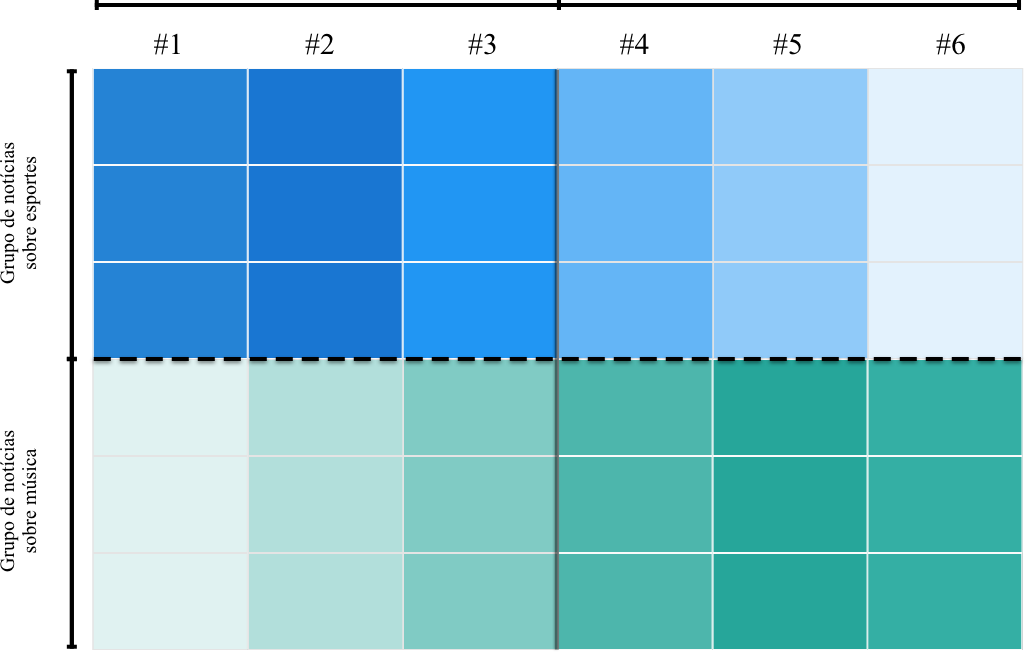
\includegraphics[width=3in]{img/sistema0.png}}\quad
%        \subfigure[ ]{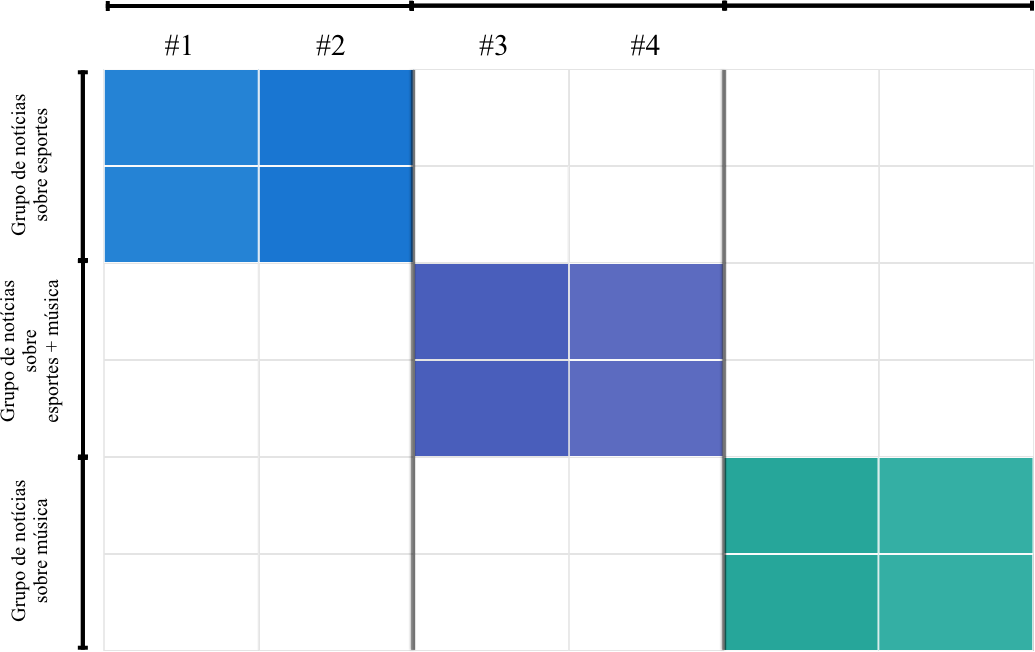
\includegraphics[width=3in]{img/sistema1.png}}
%       }
% \mbox{
%        \subfigure[ ]{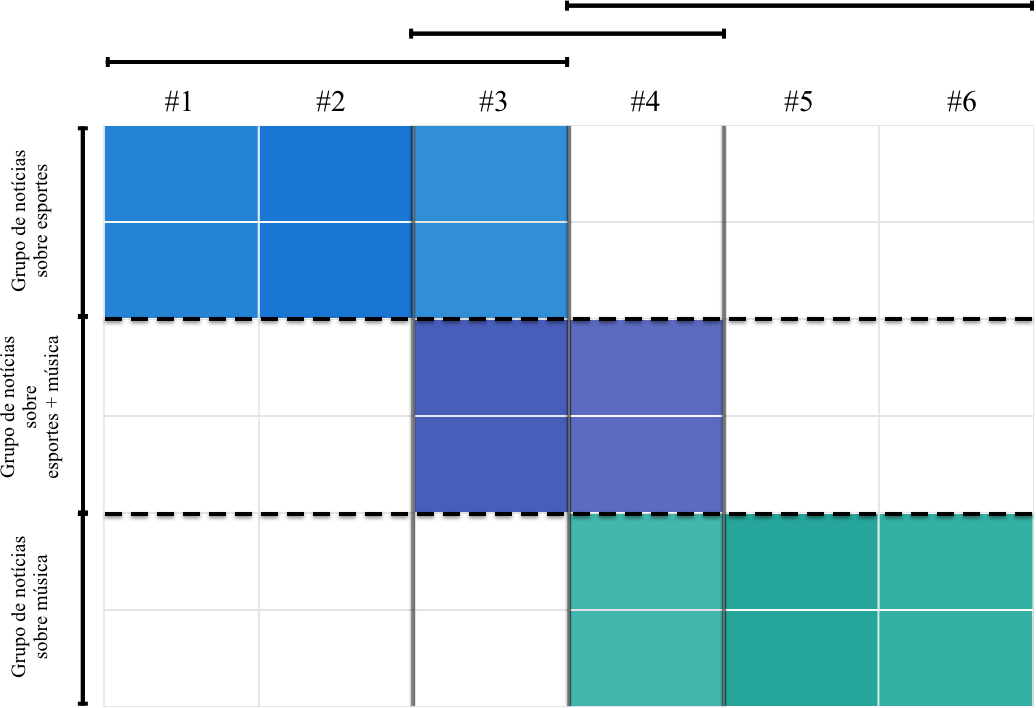
\includegraphics[width=3in]{img/sistema2.png}}\quad
%        \subfigure[ ]{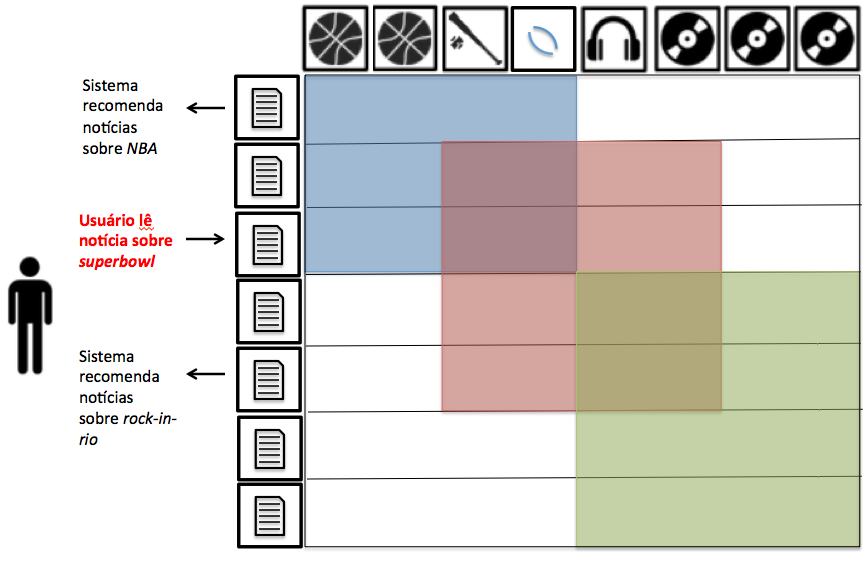
\includegraphics[width=3in]{img/sistema3.png}}
%       }
% %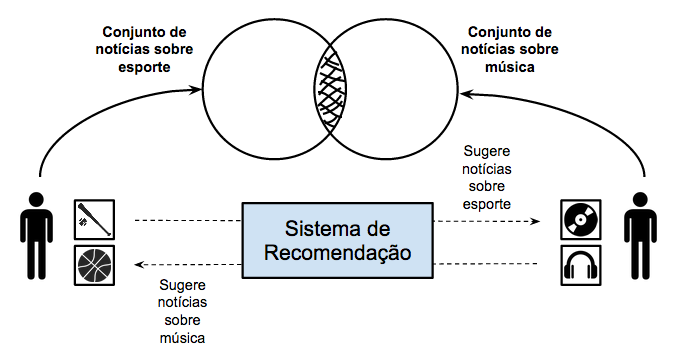
\includegraphics[width=120mm]{img/story.png}
% \caption{Representação do context de um Sistemas de Recomendação implementado a partir de análise de agrupamento com similaridade total (a) e similaridade parcial (b,c,d). Os grupos são diferenciados por cores.}
% \label{fig:story}
% \end{figure}

A associação da análise de coagrupamentos a mineração de textos é interessante por diferentes aspectos. A mineração de textos constitui-se como um problema no qual é preciso lidar com a necessidade de apresentação de resultados com boa interpretabilidade e com um espaço dos dados de alta-dimensionalidade. O primeiro problema é bem resolvido com a estratégia de coagrupamento pois os grupos de atributos que são gerados por ela podem revelar informação antes escondida nos dados \cite{Tjhi2009}, e que em um processo de agruapmento tradicional não poderiam ser, pelo menos diretamente, descobertas. Ainda segundo~\cite{Tjhi2009}, análise de coagrupamento pode apresentar bom desempenho em espaços de alta-dimensionalidade porque seu processo de agrupar atributos (características) pode ser visto com uma redução de dimensionalidade dinâmica para o espaço dos dados.

A despeito da capacidade intrínseca do processo de coagrupamento em lidar de forma diferenciada com o problema de alta-dimensionalidade, ainda se faz necessário notar que no contexto de mineração de dados, ocorre também o problema de esparsidade na representação dos dados. Assim, para implementar a estratégia de coagruapmento com alguma eficiência, é necessário adotar métodos que tenham a capacidade de lidar com esparsidade.

% tive dificuldade em justificar a escolha por fatoração de matrizes e de ligá-las à questão da esparsidade. Fiquei apenas com uma motivação. Acho que seria bom tentarmos justificar de forma mais contundente, se possível.
Dentre os diferentes métodos existentes na literatura referentes à implementação de análise de coagrupamento (\textcolor{blue}{citar artigos dos vários algoritmos que seguem outras linhas}), métodos que usam fatoração de matrizes não negativas~\cite{lee:nnmf00, lee99} têm sido vistos como uma boa alternativa a ser aplicada no contexto de mineração de textos~\cite{Xu2003, Shahnaz2006373, Yoo2010}.
%Lucas precisa olhar esses artigos direitinho para validar essas referências nesses lugares.

% ********************************************************************************************

\section{Definição do problema}

\textcolor{blue}{Eu estou entendendo que temos duas facetas do problema. Um deles é o mais obvio que é dar um jeito de descobrir os grupos com sobreposição e mostrar que é util para recomendação/textos etc. O outro é fazer a fatoração de matriz funcionar pra isso. Então acho que temos que dividir essa definição em duas partes: sobreposição nos cogrupos e fatoração funcionando nisso. Por isso dividi em duas partes, para ver se conseguimos mostrar isso.}

\subsection{Estruturas de coagrupamentos}

\textcolor{blue}{Então aqui entra a parte de mostrar as estruturas de cogrupos possívels e destacar aquela que fatoração já resolve e depois a que não resolve e a que queremos resolver. Também contextualizar no problema de recomendação ou análise de textos. Figuras precisam entrar aqui para mostra as estruturas.}

\subsection{Coagrupamento e fatorização de matrizes}

A estratégia de coagrupamento pode ser apresentada como o processo de agrupamento simultâneo de linhas e colunas em uma matriz de dados, de forma que seja possível encontrar \textbf{cogrupos} nos quais um \textbf{grupo de objetos} (linhas) associado a um deles diz respeitos a objetos que são similares entre si considerando um \textbf{grupo de atributos} (colunas), também associado ao cogrupo.

Com maior formalidade, dada uma matriz $X(N,M)$ em que $N$ é o número de linhas, $M$ o número de colunas e $x(m,n)$ é, geralmente, um número real representando a relação entre a linha $x_n$ e a coluna $y_m$, o problema de \textbf{coagruapmento} consiste em encontrar um conjunto $\mathcal{C}$ de submatrizes $G(I,J)$, onde $I=\{i_1, ..., i_r\}$ com $r \leq L$ e $J=\{j_1, ..., j_s\}$ com $s \leq C$, que maximize a similaridade entre os elementos $g\{i,j\}$.

% \cite{Franca2010,Mirkin1996,Madeira2004}.

A \textbf{esparsidade} em uma matriz é caracterizada pela existência de poucos elementos diferentes de zero ({0}). Em termos gerais, a esparsidade de uma matriz pode ser medida como a proporção de elementos iguais a zero ($0$) que ela contém. Problemas de otimização que envolvem matrizes esparsas são caracterizados por apresentarem alta complexidade combinatorial para os quais algoritmos eficientes em matrizes não esparsas tem seu desempenho bastante prejudicado.

% Sparse Convex Optimization Methods for Machine Learning. Jaggi, Martin. Tese de doutorado. ETH Zürich, 2011, p. 192

% limitação teórica: não consegui encontrar nada que me desse base para dizer: isso trabalha bem (ou melhor que outras coisas) em dados esparsos. Achei algumas coisas usando fatorizacão para problemas de recomendação por filtro e tb achei para texto, mas ninguém esta falando de esparsidade (eu acho).

\textbf{Fatorar uma matriz} consiste em encontrar duas, ou mais, novas matrizes que ao serem multiplicadas, reconstroem a matriz original. Considere uma matriz $R(N,M)$ em que $N$ é o número de linhas, $M$ o número de colunas. A fatoração desta matriz em duas novas matrizes consiste em encontrar duas matrizes $U(N,K)$ e $D(M,K)$, tal que $ R = U \times D^t = \hat{R} $. Se $K$ é escolhido tal que seja menor do que $N$ e $M$, então é dito que $U$ e $D$ são representações compactas de $R$. Se a matriz R, e as suas decomposições, são não negativas, tem-se o caso de  fatorização de matriz não-negativa.

% usar o artigo da nature para justificar a nao negativa??? Ou a justificativa vem do fato do nosso problema se encaixar nessa restrição. Essa restrição deixa o problema mais fácil de resolver?

O problema de coagruapmento pode ser modelado de tal forma que a fatoração de matriz é capaz de fornecer uma aproximação da organização em cogrupos presente no conjunto de dados sob análise.

Considere que o conjunto de dados sob análise é representado pela matriz $X(N,M)$, a fatoração dessa matriz em duas (ou mais) novas matrizes $U(N,K)$ e $D(M,K)$ significa que $K$ grupos de linhas foram descobertos, de acordo com $K$ grupos de colunas.

% Colocar a figura 2 do artigo do Yoo e Choi (referenciando, e claro).

Se três matriz são geradas na fatoração, $U(N,L)$, $S(L,K)$ e $D(M,K)$ , a interpretação pode incluir uma noção de pesos (matriz $S$) que relacionam grupos de linhas e grupos de colunas, e dimensões diferentes para as matrizes $U$ e $D$ podem ser admitidas de modo que o número de grupos de linhas pode ser diferente do número de grupo de colunas.

% Colocar a figura 3 do artigo do Yoo e Choi (referenciando, e claro).

\textcolor{blue}{Imagino que agora tem que entrar uma apresentação rápida do algoritmo novo.}

% ************************************************************************

% essa ilustração deveria ser deixada para um capítulo de coagraupamento

%O problema de Biclusterização pode ser ilustrado na Figura~\ref{fig:bicluster-exp}, onde se tem um conjunto de dados que possui objetos $x_1, x_2, x_3, x_4, x_5$ e $x_6$ que são representados pelos atributos $y_1, y_2, y_3, y_4, y_5$ e $y_6$, onde $N,M = 6$.
%Na Figura~\ref{fig:bicluster-exp} também estão ilustrados dois biclusters hipotéticos: o primeiro formado pelos objetos $x_5$ e $x_6$ e todos os atributos ($y_1, \dots, y_6$), representando um bicluster com \textit{modelo global}; e o segundo formado pelos objetos $x_2, x_3, x_4$ e $x_5$ e atributos $y_4, y_5$ e $y_6$, representando um bicluster com \textit{modelo local}, que leva em consideração apenas um subconjunto dos atributos.

%\begin{figure}[h]
%\centering
%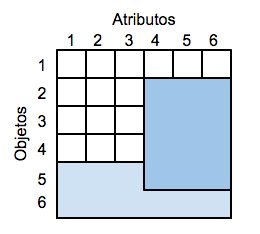
\includegraphics[width=80mm]{img/bicluster.png}
%\caption{Conjunto de dados com dois biclusters encontrados.}
%\label{fig:bicluster-exp}
%\end{figure}

% ************************************************************************

\section{Hipótese}

Fatoração de matrizes considerando a decomposição da matriz original em ... \textcolor{red}{como descrever em algo nível aqui??} ... possibilita a descoberta de cogrupos com sobreposição (de colunas); a partir das novas matrizes é possível extrar informação detalhada sobre a relação dos grupos de linhas em relação ao grupo de colunas que pode agregar valor à solução de um problema real de recomendação.

% Não estou certa de que devemos usar recomendação, talvez devessemos usar agrupamento de textos.

% ************************************************************************

\section{Objetivos}

O objetivo geral desse trabalho é propor novas estratégias, baseadas em fatoração de matrizes, que sejam capazes de descobrir cogrupos com sobreposição (de coluna) em uma matriz de valores reais positivos.

%A clusterização, nesse contexto, deve atuar como estratégia de organização do conteúdo textual, agrupando itens em biclusters.Sendo que a partir da observação dos interesses do usuário e dos biclusters à que estes itens pertencem, é possível organizar a lista recomendação com itens desses biclusters que esse usuário ainda não interagiu.

Assim, com o intuito de melhor definir o contexto de estudo deste trabalho, foram estabelecidos os seguintes objetivos específicos:

\begin{itemize}

% se nomearmos as estratégias podemos chamá-las pelo nome aqui

\item apresentação de uma derivação formal, incluindo uma prova de convergência, para a estratégia de coagrupamentos usando fatoração de matrizes não-negativas capaz de lidar com matrizes binárias;

\item apresentação de uma derivação formal para a estratégia de coagrupamento usando atoração de matrizes não negativas capaz de lidar com matrizes de valores reais positivos;

\item apresentar experimentos que ilustram a eficácia das estratégias propostas considerando dados sintéticos e dados reais, mostrando inclusive o potencial de descoberta de informações de valor diferenciado para as aplicações em teste (recomendação baseada em conteúdo textual).

% \item Levantamento do referencial teórico de SRs.
% \begin{itemize}
%  \item Levantamento do estado da arte sobre o uso de Aprendizado de Máquina na implementação de SRs baseados em conteúdo textual.
% \end{itemize}
% \item Levantamento do referencial teórico sobre Biclusterização e Mineração de Texto.
% \item Construção de um corpus de itens textuais e um conjunto de dados de recomendação.
% \item Implementação e teste dos algoritmos de Biclusterização sobre o corpus construído.
% \item Modelagem do problema de recomendação baseado em conteúdo considerando a existência de biclusters de itens.
% \item Análise da viabilidade da modelagem proposta frente ao conjunto de dados de recomendação e frente a análise qualitativa do alcance da serendipidade.
 % \item estudo das técnicas de essemble aplicadas a texto

\end{itemize}

% ************************************************************************

\section{Metodologia}

A análise exploratória da literatura especilizada foi escolhida como estratégia para a aquisição de conhecimento sobre a área de coagrupamento e fatoração de Matrizes aplicada à coagrupamento.

\textcolor{blue}{E não estou conseguindo encontrar uma forma de descrever a parte referente à concepção das estratégias propostas e também não sei como definir as estratégias referente às derivações.}

%Já para o levantamento do estado da arte em SRs baseados em conteúdo textual e sobre a aplicação de técnicas de Aprendizado de Máquina, mais especificamente clusterização, em SRs baseados em conteúdo textual, optou-se por aplicar a técnica de construção de revisões sistemáticas. A Revisão Sistemática (RS) é um tipo de revisão bibliográfica documentada, na qual cada passo da pesquisa é registrado seguindo critérios rigorosos, e portanto permitindo facilmente a auditoria e reprodução da pesquisa. Segundo \citeonline{Kitchenham2004}, a RS é um meio de avaliar, identificar e interpretar todas as pesquisas relevantes disponíveis em uma determinada área com base em questões de pesquisa. A RS que relaciona Aprendizado de Máquina e SRs se faz útil uma vez que a aplicação de Biclusterização como estratégia de resolução do problema é o núcleo deste projeto. Apesar de estar sendo realizada uma RS, neste documento optou-se por apresentar uma revisão bibliográfica no formato simples, isto é, sem os processos detalhados em \citeonline{Kitchenham2004}, visto que a construção da RS ainda esta em andamento.

A fim de permitir a validação das estratégias propostas e, portanto, a verificação da  hipótese, fez-se necessário a definição de: (a) um ambiente de teste controlado, representado por uma coleção de conjuntos de dados sintéticos, contendo cada um dos conjuntos situações diferentes referentes às estrutura de coagrupamento e variações em relação à esparsidade;  (b) um contexto para realização de uma prova de conceito, no qual um conjunto de dados real foi construído.

Para a prova de conceito foi escolhido usar o conteúdo referente à notícias publicadas no portal iG\footnote{http://ig.com.br/}.
Trata-se de um portal de notícias brasileiro muito conhecido, com um volume de notícias bastante grande e com notícias categorizadas em canais, que representam os assuntos dessas notícias. Essas características conferem liberdade para a configuração de experimentos de diferentes naturezas, como experimentos considerando determinadas categorias de notícias, tipos de notícias ou datas de publicação das notícias.

A partir do conteúdo de notícias do portal iG foi construído um corpus de dados textuais, categorizados de acordo com as categorias já usadas no referido portal.
Todo o conteúdo do corpus passou por rotinas de pré-processamento comuns na área de Mineração de Texto: \textit{tokenização}, filtragem de \textit{stopwords}, remoção de sufixos (\textit{stemming}), representação da relação ``termos $\times$ documentos'' usando estratégias de frequência de termos, como TF-IDF e \textit{n-grams}.

%Leia com muito cuidado e veja se faz sentido. MUITO CUIDADO.ALTERE O QUE FOR NECESSÄRIOS TAMBÉM COM MUITO CUIDADO.
%Também, o portal iG possui informações históricas e anônimas referentes ao registro de navegação de usuários.
%Esse registro permite a construção de um conjunto de dados de preferências, que pode ser usado para realização de \textit{testes offline} entre recomendações oferecidas pela abordagem proposta e a navegação real realizada por um conjunto de usuários, utilizando métricas como precisão, revocação \cite{Jannach2011} e comparação com recomendações geradas por filtro colaborativo.

Os resultados da aplicação das estratégias de coagrupamento foram validados utilizando técnicas de avaliação interna, para a verificação da consistência dos biclusters encontrados \cite{Santamaria2007}, e externas \cite{Hochreiter2010}, avaliando o quanto os biclusters encontrados estão em consenso com as classes de notícias \cite{Hochreiter2010}.

\textcolor{blue}{Então precisaremos dizer aqui como fizemos a avaliação qualitativa.}

% essa parte aqui ficou bem frágil.
% Os algoritmos de análise de texto via Biclusterização deverão ser validados antes de serem aplicados ao corpus criado.
% Para isso, conjuntos de dados de referência para Biclusterização e para clusterização de texto deverão ser usados.
% Uma vez alcançada a análise dos textos via Biclusterização, o modelo de uso dos biclusters em um contexto de recomendação deverá ser delineado e analisado.
% A análise deverá estar baseando tanto em comparações com o conjunto de dados de recomendação do portal iG quando por análise qualitativa do alcance da serendipidade.

%Para conhecer a área de Sistemas de Recomendação foi realizado um levantamento do referencial teórico através da análise exploratória de livros e artigos do tipo revisão bibliográfica \cite{Adomavicius2005,Lops2011,Ricci2011,Ricci22011,Jannach2011,Burke2002}, o que permitiu, em seguida, o aprofundamento na área de SRs.
%Para o aprofundamento na área de SRs, foi realizada uma Revisão Sistemática de SRs baseados em conteúdo textual.
%Também foi realizado um levantamento do referencial teórico, através da análise exploratória de livros e artigos do tipo revisão bibliográfica, na área de Mineração de Dados \cite{Berry2010,Feldman2006,Miner2012,Hotho2005,Weiss2010}, para que fosse possível realizar a análise e estruturação do conteúdo não-estruturado, presentes nas notícias.

%Isso tudo tem que vir no capitulo da propsota, como eu disse, aqui é não é um momento de relatar atividades realizadas.
% Sendo assim, com a extração das notícias do portal iG\footnote{http://ig.com.br/} através de um \textit{web crawler} utilizando a linguagem python\footnote{https://www.python.org/}, foi possível construir o corpus iG (Subseção~\ref{subsec:corpusig}) de notícias.
%As notícias foram capturadas a partir de uma página de início, fornecida para o \textit{web crawler}, que era selecionada a fim de equalizar a distribuição de notícias por ano e por assunto. Este trabalho também conta com uma base de cliques em notícias (Subseção~\ref{subsec:basecliquesig}), doada pelo portal de notícias iG.

%idem
%Para aplicação dos algoritmos de Biclusterização, foi realizado um levantamento do referencial teórico, através da análise exploratória de livros, artigos do tipo revisão bibliográfica e artigos que se referem à criação dos algoritmos \cite{Cheng2000,Tanay2005,Madeira2004,Santamaria2007,Kluger2003,Prelic2006}.

%Para gerar conhecimento do corpus iG, serão aplicados algoritmos de Biclusterização que estão sendo implementados\footnote{https://github.com/lucasbrunialti/biclustering-experiments} nos textos das notícias processados e representados por diversas estratégias (TF-IDF, TF-IDF normalizado e n-gramas). Assim, será possível avaliar o resultado dos algoritmos utilizando a base de dados de cliques iG.

% ************************************************************************

\section{Organização do documento}

Esta dissertação é composta por \textcolor{red}{XXX} capítulos incluindo esta introdução. Os demais capítulos estão divididos em duas partes: a primeira é dedicada a explorar a estratégia  de coagrupamento implementada com algoritmos baseadas em fatoração de matrizes; a segunda é dedicada a explorar o contexto de sistemas de recomendação baseados em conteúdo textual a partir da aplicação das estratégias de coagrupamento estudadas.

No capítulo~\ref{ch:conceitos} são apresentados os principais conceitos referentes à área de coagrupamentos. \textcolor{blue}{Especificar mais detalhes ... ... }

Estratégias de fatorização de matrizes aplicadas à coagrupamentos são discutidas no capítulo .....

A principal contribuição deste trabalho, as estratégias ... ...., é apresentada em detalhes no capítulo ... ...

% e então organizar a segunda parte

% ************************************************************
% ************************************************************
% ************************************************************

\chapter{Conceitos Fundamentais}
\label{ch:conceitos}

Técnicas e algoritmos de Biclusterização são usadas, principalmente, no contexto de expressão genética.
No entanto, algoritmos de Biclusterização se fazem úteis quando se deseja encontrar \textit{modelos locais}.
Ou seja, enquanto algoritmos de clusterização têm o intuito de encontrar \textit{modelos globais}, que geram grupos de dados levando em consideração todas as características, algoritmos de Biclusterização geram grupos de dados em que as características tem alta correlação \cite{Franca2010,Madeira2004}.

Para a descrição do problema formal de Biclusterização usa-se a seguinte definição \cite{Madeira2004}: seja uma matriz $A$, de dimensão $N \times M$, um conjunto de linhas $X = \{ x_1, \dots, x_n, \dots, x_N \}$ e um conjunto de colunas $Y = \{ y_1, \dots, y_m, \dots, y_M \}$, em que $a_{nm}$ geralmente é um número real e representa a relação entre a linha $x_n$ e a coluna $y_m$; o problema de Biclusterização é encontrar biclusters, que são submatrizes de $A$, denotados por $A_{IJ}$, em que $I \subseteq X$ e $J \subseteq Y$.
Assim, o bicluster $A_{IJ}$ é um grupo dos objetos em $I$, perante as características com alta correlação $J$.

\section{Tipos de biclusters}
\label{sec:tiposbic}

Como a definição de bicluster não inclui uma prévia estrutura da matriz $A$ e dos biclusters $A_{IJ}$, diversos algoritmos propostos na literatura diferem quanto ao tipo de bicluster que são capazes de encontrar.
Uma taxonomia dos tipos de biclusters é proposta por \citeonline{Madeira2004}:
 \begin{itemize}
  \item \textit{Biclusters com valores constantes}, se trata de biclusters em que todos os valores de $A_{IJ}$ são constantes: $a_{ij} = \mu, \forall i,j \in I,J$, onde $\mu$ é um valor constante dentro de $A_{IJ}$. Porém, em conjuntos de dados reais, esses biclusters estão presentes com algum tipo de ruído $\mu + \eta_{ij}$, onde $\eta_{ij}$ é o ruído associado com os valures de $\mu$ e $a_{ij}$ \cite{Madeira2004}.
  \item \textit{Biclusters com valores constantes nas linhas ou colunas}, se trata de biclusters com valores constantes nas linhas: $a_{ij} = \mu + \alpha_i, \forall i,j \in I,J$ ou $a_{ij} = \mu \cdot \alpha_i, \forall i,j \in I,J$, onde $\alpha_i$ é um fator aditivo ou multiplicativo para cada linha; ou ainda biclusters com valores constantes nas colunas: $a_{ij} = \mu + \beta_j, \forall i,j \in I,J$ ou $a_{ij} = \mu \cdot \beta_j, \forall i,j \in I,J$, onde $\beta_j$ é um fator aditivo ou multiplicativo para cada coluna \cite{Madeira2004}.
  \item \textit{Biclusters com valores coerentes}, em que são considerados valores próximos entre si (coerentes) para definição de um bicluster: $a_{ij} = \mu + \alpha_i + \beta_j, \forall i,j \in I,J$, ou $a_{ij} = \mu' \cdot \alpha_i' \cdot \beta_j', \forall i,j \in I,J$, sendo que se $\mu = \log \mu'\implies \alpha_i = \alpha_i', \beta_j = \beta_j'$ \cite{Madeira2004}.
  \item \textit{Biclusters com evoluções coerentes}, têm seus valores com evoluções coerentes, por exemplo, um bicluster com $a_{i4} \leq a_{i3} \leq a_{i2} \leq a_{i1}$ tem valores com evolução coerente na coluna \cite{Madeira2004}. Seus valores podem ser gerados por uma função geradora de valores com evolução coerente $a_{ij} = g(a_{ij}), \forall i,j \in I,J$, sendo $g(\cdot)$ não linear e não constante, para que o tipo de bicluster não seja classificado nos casos anteriores.
 \end{itemize}

Os biclusters também diferem quanto as suas estruturas. Cada algoritmo usado para implementar Biclusterização faz uma suposição da estrutura de biclusters que é capaz de encontrar.
A Figura~\ref{fig:bicstruct} sumariza as diferentes estruturas de biclusters, com as linhas e colunas ordenadas para permitir a visualização dos biclusters por meio do mapa de calor dos valores de $A$, sendo os biclusters $A_{IJ}$ representados por cores sólidas e o fundo da matriz ruído.
% Os tipos de estruturas são: Bicluster único, tem apenas um bicluster na matriz (Figura~\ref{fig:bicstruct-a}); Bicluster com linhas e colunas exclusivas

% Para melhorar esse figura, deixe na figura apenas as letras (a), (b) etc e faça uma legenda. Acho que você pode usar \caption*{} em cima do \caption{} para fazer a legenda. Ou crie um parágrafo para explicar as letras na figura. Acho que aaté fica mais simpático fazer um parágrafo, pois pode explicar com mais cuidado.

% \begin{figure}[h]
%     % \captionsetup[subfigure]{labelformat=simple}
%     \centering
%     \begin{subfigure}[b]{0.3\textwidth}
%             
\includegraphics[width=30mm]{img/a-bic-struct.png}
%             \caption{Bicluster único}
%             \label{fig:bicstruct-a}
%     \end{subfigure}
%     ~
%     \centering
%     \begin{subfigure}[b]{0.3\textwidth}
%             
\includegraphics[width=30mm]{img/b-bic-struct.png}
%             \caption{Biclusters com linhas e colunas exclusivas}
%             \label{fig:bicstruct-b}
%     \end{subfigure}
%     ~
%     \centering
%     \begin{subfigure}[b]{0.3\textwidth}
%             
\includegraphics[width=30mm]{img/c-bic-struct.png}
%             \caption{Biclusters com estrutura de tabuleiro de xadrez}
%             \label{fig:bicstruct-c}
%     \end{subfigure}
%     ~
%     \centering
%     \begin{subfigure}[b]{0.3\textwidth}
%             
\includegraphics[width=30mm]{img/d-bic-struct.png}
%             \caption{Biclusters com linhas exclusivas}
%             \label{fig:bicstruct-d}
%     \end{subfigure}
%     ~
%     \centering
%     \begin{subfigure}[b]{0.3\textwidth}
%             
\includegraphics[width=30mm]{img/e-bic-struct.png}
%             \caption{Biclusters com colunas exclusivas}
%             \label{fig:bicstruct-e}
%     \end{subfigure}
%     ~
%     \centering
%     \begin{subfigure}[b]{0.3\textwidth}
%             
\includegraphics[width=30mm]{img/f-bic-struct.png}
%             \caption{Biclusters sem sobreposição com estrutura em árvore}
%             \label{fig:bicstruct-f}
%     \end{subfigure}
%     ~
%     \centering
%     \begin{subfigure}[b]{0.3\textwidth}
%             
\includegraphics[width=30mm]{img/g-bic-struct.png}
%             \caption{Biclusters sem sobreposição e não exclusivos}
%             \label{fig:bicstruct-g}
%     \end{subfigure}
%     ~
%     \centering
%     \begin{subfigure}[b]{0.3\textwidth}
%             
\includegraphics[width=30mm]{img/h-bic-struct.png}
%             \caption{Biclusters com sobreposição com estrutura hierarquica}
%             \label{fig:bicstruct-h}
%     \end{subfigure}
%     ~
%     \centering
%     \begin{subfigure}[b]{0.3\textwidth}
%             
\includegraphics[width=30mm]{img/i-bic-struct.png}
%             \caption{Biclusters com sobreposição arbitrariamente posicionados}
%             \label{fig:bicstruct-i}
%     \end{subfigure}
%     \caption{Diferentes estruturas de biclusters, quadrados e retângulos com cores sólidas representam biclusters e o fundo representa ruído.}% (Adaptado de \cite{Madeira2004})}
%     \label{fig:bicstruct}
% \end{figure}

\section{Algoritmos para Biclusterização}

Diversos algoritmos para encontrar biclusters, de diferentes tipos e estruturas, foram propostos na literatura \cite{Tanay2005,Madeira2004}.

Um dos algoritmos de Biclusterização mais comum e simples. que encontra biclusters com valores coerentes, em estrutura com sobreposição e arbitrariamente posicionados, é o \textit{Coupled Two-way Clustering} (CTWC) \cite{Getz2000}. O algoritmo CTWC é capaz de encontrar biclusters através da clusterização de objetos e atributos (linhas e colunas), separadamente.
O algoritmo de clusterização usado por \citeonline{Getz2000} foi o \textit{Superparamagnetic Clustering} (SPC), o qual é capaz de determinar o número de clusters automaticamente, e com uma estratégia de clusterização hierárquica \textit{top-down} é capaz de gerar clusters estáveis \cite{Getz2000}.
O SPC tem como entrada uma matriz de similaridade e um parâmetro temperatura, que controla o quão estáveis serão os clusters que o algoritmo gerará.
Assim, o CTWC encontra clusters estáveis de linhas e colunas através do SPC, e iterativamente executa o SPC nos clusters de linhas e colunas encontrados, mantendo na memória um par do subconjunto de linhas e do subconjunto de colunas (biclusters), assim como os clusters estáveis de linhas e colunas, separadamente.
% O algoritmo se inicia com dois subconjuntos: um para exemplos (linhas) $I = \{ X \}$ e um para características (colunas) $J = \{ Y \}$, então, através do algoritmo de SPC

Já o algoritmo de \citeonline{Cheng2000} é capaz de encontrar o mesmo tipo de bicluster que o algoritmo CTWC, porém usando uma estratégia gulosa: biclusters com valores coerentes e estrutura com sobreposição e arbitrariamente posicionados. Este algoritmo esta sendo objeto de estudo desse projeto de mestrado para aplicação em dados textuais e por isso segue aqui descrito em mais detalhes.
Nesse algoritmos, para encontrar biclusters, ou $\delta$-biclusters, na matriz $A$, os autores definem o \textit{Resíduo Quadrático Médio} (RQM):
\begin{equation}
\begin{split}
    H_{IJ} = \frac{1}{|I||J|} \displaystyle\sum_{i,j \in I,J} (a_{ij} - a_{iJ} - a_{Ij} + a_{IJ})^2 \\
    H_{iJ} = \frac{1}{|J|} \displaystyle\sum_{j \in J} (a_{ij} - a_{iJ} - a_{Ij} + a_{IJ})^2 \\
    H_{Ij} = \frac{1}{|I|} \displaystyle\sum_{i \in I} (a_{ij} - a_{iJ} - a_{Ij} + a_{IJ})^2
\end{split}
\end{equation}
em que
\begin{equation}
    a_{iJ} = \frac{1}{|J|} \displaystyle\sum_{j \in J} a_{ij},\quad a_{Ij} = \frac{1}{|I|} \displaystyle\sum_{i \in I} a_{ij},\quad a_{IJ} = \frac{1}{|I||J|} \displaystyle\sum_{i,j \in I,J} a_{ij}
\end{equation}
onde $H_{IJ}$ é o RQM de uma submatriz $A_{IJ}$, $H_{iJ}$ o RQM da linha $i$, $H_{Ij}$ o RQM da coluna $j$, $a_{iJ}$ a média dos valores da linha $i$, $a_{Ij}$ a média dos valores da coluna $j$ e $a_{IJ}$ a média dos valores da submatriz $A_{IJ}$, definida pelos subconjuntos $I$ e $J$.

Então, um bicluster perfeito $A_{IJ}$ teria o RQM $H_{IJ} = 0$, pois $a_{ij} = a_{ij}, \forall i,j \in I,J$, fazendo $a_{iJ} = a_{Ij} = a_{IJ}$. No entanto, se apenas minizar o RQM, um bicluster com apenas um elemento seria perfeito, o que pode não refletir a realidade. Além disso, em conjunto de dados reais existe ruído, podendo esconder o bicluster perfeito.

Para encontrar biclusters, ou $\delta$-biclusters, \citeonline{Cheng2000} usam uma estratégia gulosa que retira linhas e colunas, visando a minimização do RQM, respeitando um parâmetro $\delta$, que é calibrado pelo usuário. Então, um bicluster é encontrado quando o RQM de uma submatriz $A_{IJ}$ é $H_{IJ} \leq \delta$, para algum $\delta \geq 0$. As etapas de remoções de elementos da matriz são apresentadas nos algoritmos 1 e 2.

% \begin{algorithm}[H]
% \label{algo:cc1}
%  \KwData{$A, I, J, \delta$}
%  \KwResult{$I,J$ onde $H_{IJ} \leq \delta$}
%  \While{$H_{IJ} > \delta$}{
%   encontre a linha $l_{max} = \operatorname*{arg\,max}_{i \in I} H_{iJ}$\;
%   encontre a coluna $c_{max} = \operatorname*{arg\,max}_{j \in J} H_{Ij}$\;
%   \eIf{$l_{max} > c_{max}$}{
%    remova $l_{max}$ do subconjunto $I$\;
%    }{
%    remova $c_{max}$ do subconjunto $J$\;
%   }
%  }
%  \caption{Remove uma linha ou coluna a cada iteração.}
% \end{algorithm}

% \begin{algorithm}[H]
% \label{algo:cc2}
%  \KwIn{$A, I, J, \delta, \alpha$}
%  \KwOut{$I,J$ onde $H_{IJ} \leq \delta$}
%  \While{$H_{IJ} > \delta$}{
%   remova $i \in I$ onde $H_{iJ} > \alpha \cdot H_{IJ}$\;
%   remova $j \in J$ onde $H_{Ij} > \alpha \cdot H_{IJ}$\;
%   encontre a coluna $c_{max} = \operatorname*{arg\,max}_{j \in J} H_{Ij}$\;
%   \If{não houve nenhuma remoção}{
%    chame o algoritmo 1
%   }
%  }
%  \caption{Remove múltiplas linhas e colunas de $A$ a cada iteração.}
% \end{algorithm}

O algoritmo 2 é usado para acelerar o processo de busca de um $\delta$-bicluster, convergindo mais rapidamente para uma solução quanto maior for o parâmetro $\alpha$, em que $\alpha \geq 0$. Ainda, para amenização do problema de encontrar $\delta$-biclusters perfeitos com apenas um elemento, ou poucos elemento, é utilizado o algoritmo 3, que adiciona nós sem aumentar o RQM do bicluster.

% deu problema nessas referencias cruzadas, verifique.

% \begin{algorithm}[h]
% \label{algo:cc3}
%  \KwIn{$A, I, J$}
%  \KwOut{$I',J'$ onde $H_{I'J'} \leq H_{IJ}$}
%  \While{$H_{IJ} > \delta$}{
%   compute $a_{iJ}$ e $a_{Ij}$ para todo $i,j$ e $H_{IJ}$\;
%   remova $j \notin J$ onde $\frac{1}{|I|} \sum_{j \in J} (a_{ij} - a_{iJ} - a_{Ij} + a_{IJ})^2 \leq H_{IJ}$\;
%   recompute $a_{iJ}$ e $H_{IJ}$\;
%   remova $i \notin I$ onde $\frac{1}{|J|} \sum_{i \in I} (a_{ij} - a_{iJ} - a_{Ij} + a_{IJ})^2 \leq H_{IJ}$\;
%   \If{não houve nenhuma adição}{
%    $I' \longleftarrow I$\;
%    $J' \longleftarrow J$\;
%   }
%  }
%  \caption{Adiciona linhas e colunas de $A_{IJ}$ a cada iteração.}
% \end{algorithm}

Por fim, o algoritmo 4 é a consolidação dos algoritmos 3, 2 e 1 e a iteração para encontrar $k$ $\delta$-biclusters, um a um, sendo $k$ fornecido pelo usuário.

% \begin{algorithm}[h]
% \label{algo:cc4}
%  \KwIn{$A, k, \delta, \alpha$}
%  \KwOut{$k$ $\delta$-biclusters}
%  $A' \leftarrow A$\;
%  \For{$1$ \KwTo $k$}{
%    $B \leftarrow$ algoritmo 2 com $A', \delta, \alpha$\;
%    $C \leftarrow$ algoritmo 1 com $B, \delta$\;
%    $D \leftarrow$ algoritmo 3 com $A, C$\;
%    reporte $D$ como uma solução\;
%    adicione ruído em $A'$ para a submatriz $D$\;
%  }
%  \caption{Algoritmo Cheng \& Church, encontra $k$ $\delta$-biclusters.}
% \end{algorithm}

% Algoritmo Spectral (?)

Além dos algoritmos apresentados, existem outros algoritmos que são capazes de encontrar outros tipos de biclusters (Seção~\ref{sec:tiposbic}), além de serem recentes \cite{Franca20102,Yang2013,Hochreiter2010,Cabanes2012}, mostrando que ainda há interesse na área de pesquisa de Biclusterização.

 \section{Avaliação de Biclusterização}

Para determinar parâmetros, descobrir a qualidade e/ou estabilidade dos biclusters encontrados por algoritmos, é necessário estabelecer métricas de avaliação. Existem duas maneiras de avaliar biclusters \cite{Hochreiter2010}: \textit{interna}, usa os dados dos resultados dos algoritmos, juntamente com métricas de qualidade e/ou estabilidade, para avaliar as soluções geradas; \textit{externa}, utiliza os dados reais das soluções de biclusters de um conjunto de dados, usando estratégias para comparação, obtendo assim, maior confiança nas soluções.

A avaliação interna pode não ser tão precisa quanto a avaliação externa, porém é útil para descobrir parâmetros ótimos. Apesar de \citeonline{Prelic2006} sugerirem não usar avaliações internas, por não estar claro como extender noções de separação e homogeinidade, \citeonline{Santamaria2007} descreveu métricas de consistência para verificando se um bicluster é consistente com a sua definição, seja aditiva, multiplicativa e/ou constante, fazendo uma comparação dos elementos do bicluster:
\begin{equation}
\begin{split}
C_l(A_{IJ}) = \frac{1}{|I|} \displaystyle\sum_{i = 1}^{|I| - 1} \displaystyle\sum_{j = i + 1}^{|I|} \sqrt{ \displaystyle\sum_{k = 1}^{|J|} (a_{ik} - a_{jk})^2 } \\
C_c(A_{IJ}) = \frac{1}{|J|} \displaystyle\sum_{i = 1}^{|J| - 1} \displaystyle\sum_{j = i + 1}^{|J|} \sqrt{ \displaystyle\sum_{k = 1}^{|I|} (a_{ki} - a_{kj})^2 }
\end{split}
\end{equation}
em que $C_l(A_{IJ})$ é o índice de consistência das linhas do bicluster $A_{IJ}$ e $C_c(A_{IJ})$ é o índice de consistência das colunas do bicluster $A_{IJ}$. Ainda, a consistência do bicluster inteiro $C$ pode ser definida pela média:
\begin{equation}
C(A_{IJ}) = \frac{|I| \cdot C_l + |J| \cdot C_c}{|I| + |J|}
\end{equation}

Uma das métricas externas que são usadas para comparar biclusters encontrados com biclusters reais em um conjunto de dados, é a métrica \textit{concensus score} \cite{Hochreiter2010}. Essa métrica calcula a maximização das similaridades entre biclusters encontrados e reais, usando o \textit{índice de Jaccard} como medida de similaridade e o algoritmo Húngaro para solucionar o problema de maximização. A saída da avaliação é um $\textit{score} \in [0,1]$, em que $0$ significa que os biclusters comparados são totalmente diferentes, e $1$ o inverso.

% ************************************************************
% ************************************************************
% ************************************************************
% ************************************************************

\chapter{Fatoração de matrizes}
\label{ch:fatoracao}

% TODO: resgatar fatoração de matrizes tradicionais

\section{Non-negative Matrix Factorization}

% justificar non-negative
% NMF baseado em partes (ver tese RHO)
% NMF formalização

\section{Fatoração de Matrizes Não-Negativas para Coclustering}

Algoritmos de coclustering baseados em Fatoração de Matrizes Não-negativas (\textit{Non-negative Matrix Factorization} - NMF) podem ser úteis em múltiplos contextos, aparecendo em diversos tipos de aplicações, como clusterização de genes e análise de microarray em bioinformática, filtragem colaborativa em sistemas de recomendação, e clusterização de documentos em mineração de textos. % TODO Citação para cada um
Isso acontece pois muitas das representações usadas nessas aplicações se apresentam em tuplas contendo um par de elementos, cada um pertencendo a um conjunto finito~\cite{Long2005}.
Por exemplo, na aplicação de clusterização de documentos em mineração de textos, usa-se, comumente, dois conjuntos: documentos e palavras, sendo cada observação representada pela contagem de uma determinada palavra em um determinado documento.
Note ainda, que conjuntos de dados utilizados nos contextos citados, apresentam-se como uma matriz de dados positiva, expondo outra característica em que NMF podem ser úteis para esses tipos de dados.
Além disso, essas técnicas, por reduzir a dimensionalidade orinal do conjunto de dados, são capazes de lidar com dados de alta dimensionalidade e/ou esparsos, que são geralmente presentes nessas aplicações.

% TODO como melhorar a notação
\textcolor{red}{Formalizando, algoritmos de Coclusterização baseados em Fatoração de Matrizes Não-negativas, têm como entrada uma matriz de dados $X$ que representa uma aplicação em algum contexto, sendo $X \in \mathbb{R}^{n \times m}_{+}$, contendo números reais positivos com $n$ linhas e $m$ colunas
Esta matriz é formada por um conjunto de vetores de linhas $\mathcal{X} = \{ x_{1 \cdot}, \dots, x_{n \cdot} \}$ e um conjunto de vetores de colunas ${\mathcal{Y}} = \{ y_{\cdot 1}, \dots, y_{\cdot m} \}$, e cada observação representada por $x_{ij}$, que é justamente um valor da matriz $X$.}

\textcolor{red}{O objetivo é particionar $\mathcal{X}$ em $k$ grupos de linhas, denotados pelos subconjuntos ordenados $I_p \subseteq \mathcal{X}$, e $l$ grupos de colunas, subconjuntos $J_q \subseteq \mathcal{Y}$, podendo assim, pela junção desses subconjuntos, formar cogrupos $(I_p, J_q)$.
Note então, que os algoritmos tradicionais presentes na literatura são capazes de formar $k l$ cogrupos.}

As próximas subseções irão mostrar definições dos algoritmos de coclusterização baseados em NMF presentes na literatura, assim como estratégias usadas para selecionar os cogrupos mais relevantes dos $k l$ possíveis.

\subsection{Decomposição de Valores em Blocos para Coclustering}
\label{subsec:bvd}

Um dos primeiros algoritmos propostos na literatura para a resolução do problema de \textit{coclustering} baseado em NMF, é o Decomposição de Valores em Blocos (\textit{Block Value Decomposition} - BVD).
Esta decomposição recebe esse nome, justamente, por ter capacidade de encontrar estruturas em blocos na matriz de dados.
Isso é possível pois o algoritmo é capaz de explorar a relação entre linhas e colunas, através da decomposição em três matrizes, $U$ a matriz de coeficientes de linhas, $S$ a matriz com estrutura em blocos, e $V$ a matriz de coeficientes de colunas, sendo os coeficientes o grau com que cada vetor (linha ou coluna) de $X$ pertence a um grupo, e a estrutura em blocos, uma representação compacta da matriz original.
Sendo assim, multiplicando as três matrizes geradas pela fatoração, é possível reconstruir a matriz original $X$ por partes.

O objetivo é encontrar grupos de forma simultânea, sendo $k$ grupos de $\mathcal{X}$ (linhas) e $l$ grupos de $\mathcal{Y}$ (colunas) \cite{Long2005}.

A aproximação $X \approx USV^T$ é capaz de gerar diversas informações interpretáveis através da análise do resultado da fatoração.
Os valores da matriz $U$ podem ser interpretados como o grau com que cada objeto $x_{i \cdot}$ $\forall i = \{1, \dots, n\}$ pertence à um dos $k$ grupos de linhas, da mesma forma, os valores da matriz $V$ podem ser interpretados como o grau com que cada objeto $y_{\cdot j}$ $\forall j = \{1, \dots, m\}$ pertence à um dos $l$ grupos de colunas.
A matriz $S$ também permite interpretação quando são considerados os grupos formados por $U$ e $V$, cada valor $s_{pq}$ $\forall p = \{1, \dots, k\}, \forall q = \{1, \dots, l\}$ representa a intensidade em que o grupo de objetos $J_p$ e o grupo de características $J_q$ se relacionam, ou seja, fixando um grupo de objetos $I_p$, $s_{pq}$ representa a intensidade que $J_q$ colaborou para a sua formação, alternadamente, fixando um grupo de características $J_q$, $s_{pq}$ representa a intensidade na qual o grupo de objetos $I_p$ colaborou para a sua formação.

Um exemplo de fatoração em três matrizes e sua interpretação pode ser visto na Figura~\ref{fig:bvd}.

% TODO explicar melhor as figuras
\begin{figure}[H]
\centering
    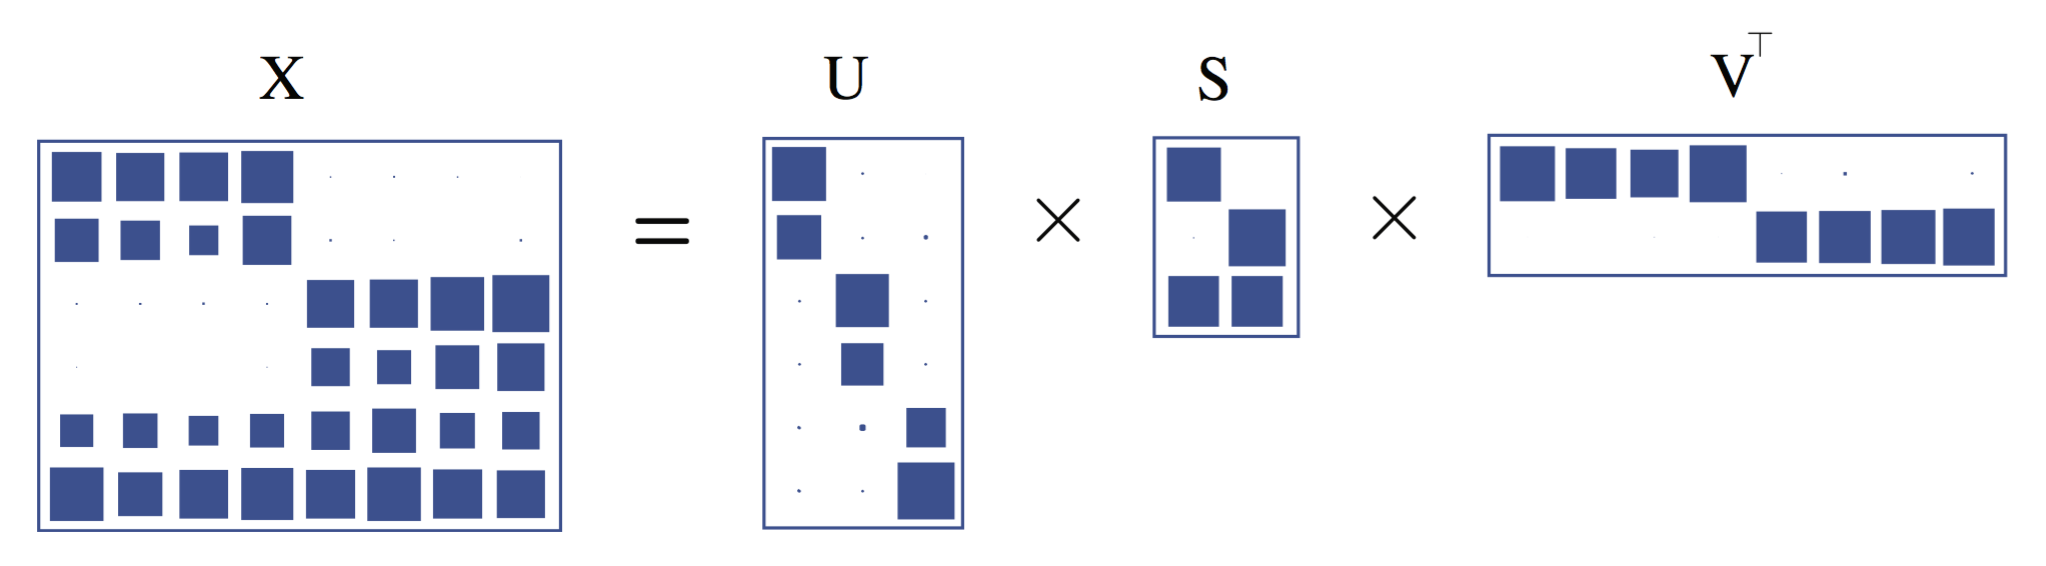
\includegraphics[width=0.7\textwidth]{img/factorizationXUSV.png}
    \caption{
        Fatoração da matriz original de dados $X$ em três outras matrizes: $U$, $S$ e $V$ (Adaptado de \citeonline{Yoo2010}).
    }
    \label{fig:bvd}
\end{figure}

Note ainda, que é possível obter os protótipos responsáveis por cada parte da reconstrução da matriz original $X$.
Os vetores das colunas de $(US)$ são vetores base (protótipos de colunas), geradores de vetores de colunas de $X$.
Assim como os vetores de linhas de $(SV^T)$, que são vetores base (protótipo de linhas), geradores de vetores e linhas de $X$.
A Figura~\ref{fig:bvd:reconstruction} mostra um exemplo de como os protótipos são responsáveis pela reconstrução de $X$.

\begin{figure}[H]
\centering
    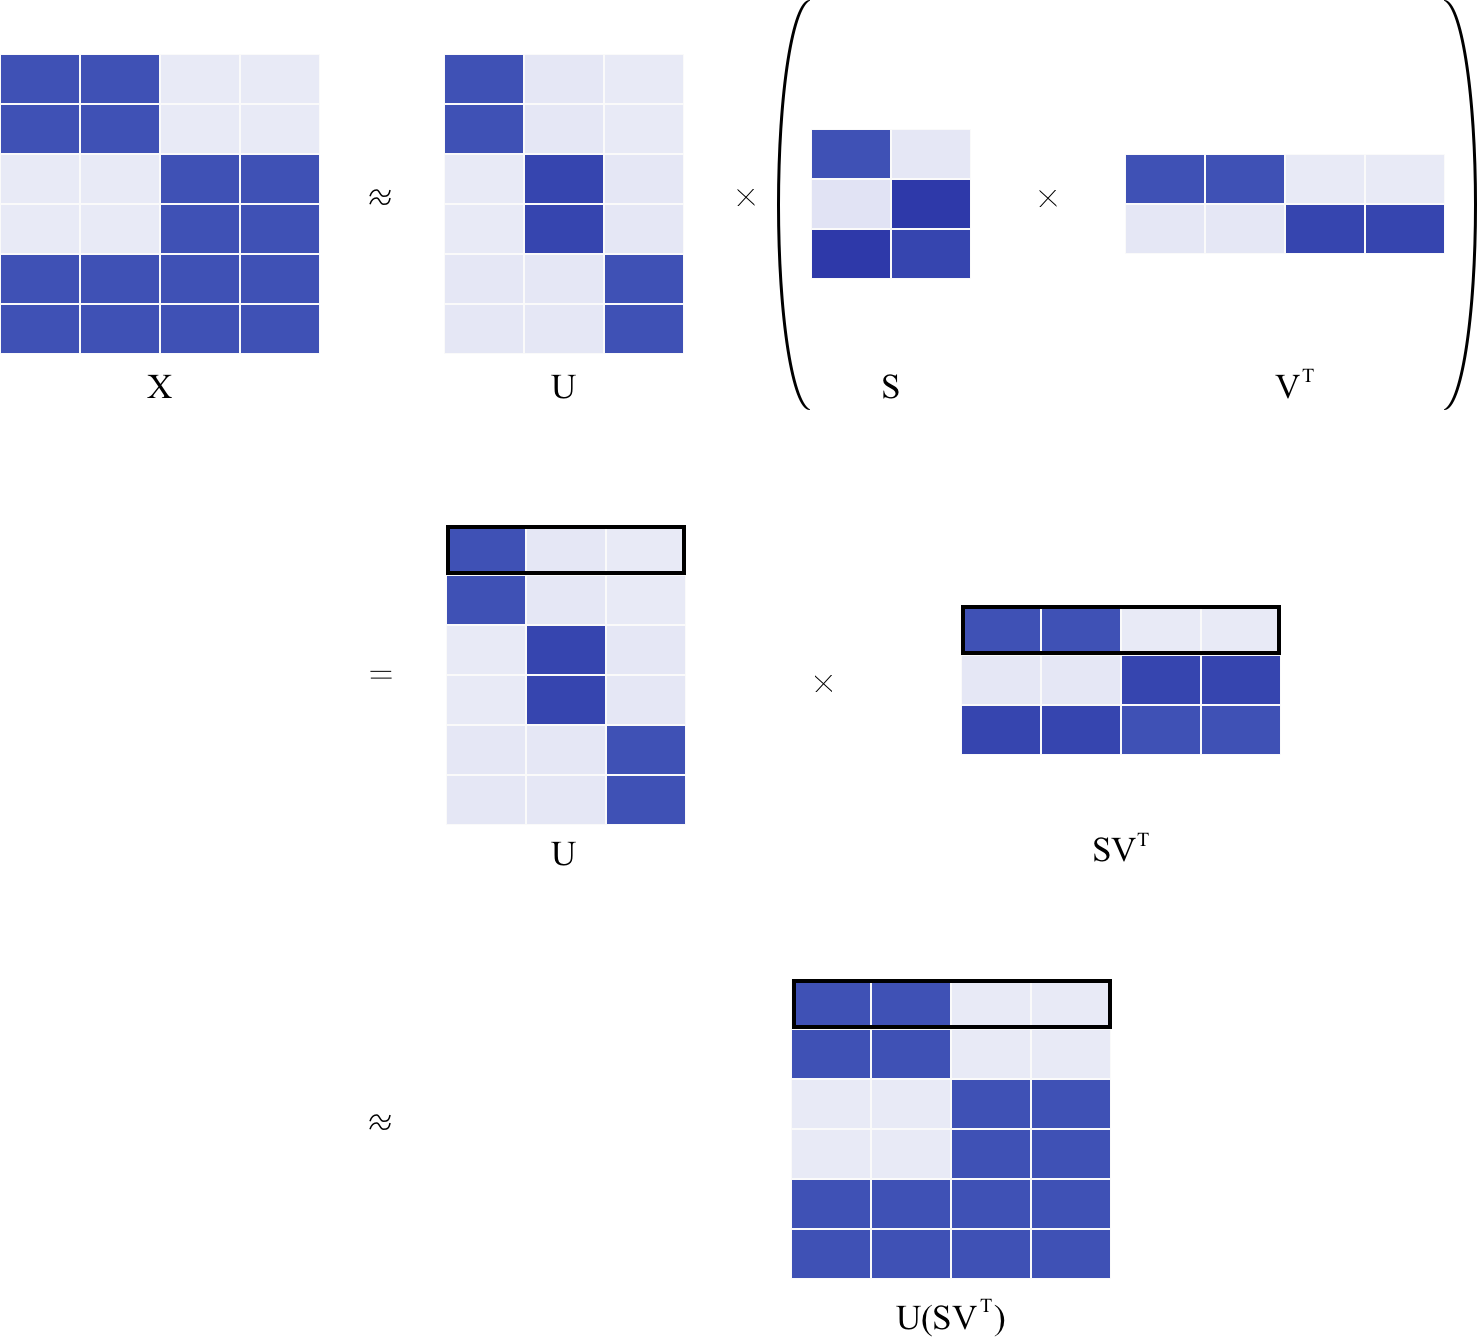
\includegraphics[width=0.7\textwidth]{img/reconstruction.png}
    \caption{
        A reconstrução da primeira linha $x_{1 \cdot}$ de $X$, através da multiplicação da matriz indicadora de grupos de linhas $U$ pela matriz dos protótipos de linhas $(S V^T)$. %que para a primeira linha seleciona apenas o primeiro protótipo,
    }
    \label{fig:bvd:reconstruction}
\end{figure}

Apresentando o problema formalmente, temos:

\begin{problem}[Problema de Decomposição de Valores em Blocos]
\label{def:bvd:problem}
\begin{equation}
    \begin{array}{lclcl}
        \displaystyle \mathcal{F}_1(U, S, V) & = & \displaystyle \min_{U, S, V} & \norm{X - USV^T}^{2}_{F} \\
                                           &   & \text{suj. a}                & U \geq 0,                \\
                                           &   &                              & S \geq 0,                \\
                                           &   &                              & V \geq 0
    \end{array}
\end{equation}
\end{problem}

onde $U \in \mathbb{R}^{n \times k}_{+}$, $S \in \mathbb{R}^{k \times l}_{+}$, $V \in \mathbb{R}^{m \times l}$ e $\norm{\cdot}_F$ denota a norma de Frobenius para matrizes.

Introduzindo a função lagrangeana, associada à $\mathcal{F}_1$:
\[
    \displaystyle \mathcal{L}(U, S, V, \Lambda_1, \Lambda_2, \Lambda_3) = \norm{X - USV^T}^{2}_{F} - tr(\Lambda_1 U^T) - tr(\Lambda_2 S^T) - tr(\Lambda_3 V^T) \\
\]

onde $\Lambda_1 \in \mathbb{R}^{n \times k}$, $\Lambda_2 \in \mathbb{R}^{k \times l}$ e $\Lambda_3 \in \mathbb{R}^{m \times l}$ são os multiplicadores de Lagrange.

Pela teoria de otimização não-linear com restrições, $\Theta = (U^{*}, S^{*}, V^{*}, \Lambda_{1}^*, \Lambda_{2}^*, \Lambda_{3}^*)$ será um mínimo local estacionário de $\mathcal{F}_1$, se e somente se, respeitar as condições de regularidade de \textit{Karush-Kuhn-Tucker} (KKT)~\cite{bazaraa2006}:

\begin{subequations}
    \begin{alignat}{3}
        U^* \geq 0, \quad                  && S^* \geq 0, \quad                     && V^* \geq 0                  \label{eq:bvd:kkt1} \\
        \quad                              && \nabla_{\Theta} \mathcal{L} = 0 \quad &&                             \label{eq:bvd:kkt2} \\
        \Lambda_{1}^* \odot U^* = 0, \quad && \Lambda_{2}^* \odot S^* = 0, \quad    && \Lambda_{3}^* \odot V^* = 0 \label{eq:bvd:kkt3}
    \end{alignat}
\end{subequations}

onde $\odot$ denota o produto de Hadamard.

É possível expandir as equações em~\ref{eq:bvd:kkt2}, calculando as derivadas:

\[
\begin{array}{lclclclcl}
    \nabla_U \mathcal{L} & = & U S V^{T} V S^{T}     & - & X V^{T} S^{T} & - & \Lambda_1 & = & 0 \\
    \nabla_S \mathcal{L} & = & U^{T} U S V^{T} V     & - & U^{T} X V     & - & \Lambda_2 & = & 0 \\
    \nabla_V \mathcal{L} & = & S^{T} U^{T} U S V^{T} & - & S^{T} U^{T} X & - & \Lambda_3 & = & 0
\end{array}
\]

Aplicando o produto Hadamard dos dois lados de cada uma das equações e utilizando das condições em~\ref{eq:bvd:kkt3}:
\[
\begin{array}{lclclclclcl}
    \nabla_U \mathcal{L} & = & U & \odot & U S V^{T} V S^{T}     & - & U & \odot & X V^{T} S^{T} & = & 0 \\
    \nabla_S \mathcal{L} & = & S & \odot & U^{T} U S V^{T} V     & - & S & \odot & U^{T} X V     & = & 0 \\
    \nabla_V \mathcal{L} & = & V & \odot & S^{T} U^{T} U S V^{T} & - & V & \odot & S^{T} U^{T} X & = & 0
\end{array}
\]

Desta forma, é possível resolver para $U$ de forma algébrica:
\[
\begin{array}{lclclcl}
             & U \odot U S V^{T} V S^{T}                           & = & U \odot X V^{T} S^{T} \\
    \implies & U \odot \frac{U S V^{T} V S^{T}}{U S V^{T} V S^{T}} & = & U \odot \frac{X V^{T} S^{T}}{U S V^{T} V S^{T}}
\end{array}
\]

\[
    \begin{array}{lclcl}
        \therefore & U & = & U \odot \frac{X V^{T} S^{T}}{U S V^{T} V S^{T}}
    \end{array}
\]

Da mesma maneira é possível resolver para $S$ e $V$, assim como mostram as equações~\ref{eq:bvd:updateS} e \ref{eq:bvd:updateV}, descritas no algoritmo~\ref{algo:bvd} \cite{Long2005}.
% Através da iteração do ponto fixo é possível encontrar regras para atualização multiplicativa de $U$, $S$ e $V$, assim como mostra as equações~\ref{eq:bvd:updateU}, \ref{eq:bvd:updateS} e \ref{eq:bvd:updateV}, respectivamente, assim como mostram o algoritmo~\ref{algo:bvd} \cite{Long2005}.
Considere $t$ o contador de iterações, e $U^{(t)}$, $S^{(t+1)}$ e $V^{(t+1)}$, as matrizes $U$, $S$ e $V$, na iteração $t$, respectivamente.

\begin{algorithm}
\caption{Algoritmo baseado em atualização multiplicativa para solução do BVD}
\label{algo:bvd}
    \begin{algorithmic}[1]
        \Function{BVD}{$X$, $maxIter$}
            \State \textbf{Inicialize:} $U^{(0)} \geq 0, V^{(0)} \geq 0, S^{(0)} \geq 0$ e $t \gets 0$.
            \While{(não convergiu) ou ($t \leq maxIter$)} %\Comment{We have the answer if r is 0}
                \State
                    \begin{equation}
                    \label{eq:bvd:updateU}
                        U^{(t+1)} \gets U^{(t)} \odot \frac{ X V^{(t)^T} S^{(t)^T} }{ U^{(t)} S^{(t)} V^{(t)^T} V^{(t)} S^{(t)^T} }
                    \end{equation}
                \State
                    \begin{equation}
                    \label{eq:bvd:updateV}
                        V^{(t+1)} \gets V^{(t)} \odot \frac{ S^{(t)^T} U^{(t+1)^T} X }{ S^{(t)^T} U^{(t+1)^T} U^{(t+1)} S^{(t)} V^{(t)^T} }
                    \end{equation}
                \State
                    \begin{equation}
                    \label{eq:bvd:updateS}
                        S^{(t+1)} \gets S^{(t)} \odot \frac{ U^{(t+1)^T} X V^{(t+1)} }{ U^{(t+1)^T} U^{(t+1)} S^{(t)} V^{(t+1)^T} V^{(t+1)} }
                    \end{equation}
                \State $t \gets t + 1$
            \EndWhile\label{euclidendwhile}
            \State \textbf{return} $U^{(t+1)}, S^{(t+1)}, V^{(t+1)}$
        \EndFunction
    \end{algorithmic}
\end{algorithm}

% \begin{theorem}[Corretude]
% \label{def:bvd:correctness}
%     As regras de atualização das equações~\ref{eq:bvd:updateU},~\ref{eq:bvd:updateV} e~\ref{eq:bvd:updateS} são corretas para resolução do problema~\ref{def:bvd:problem}, ou seja, respeitam a condição da equação~\ref{eq:bvd:kkt2}.
% \end{theorem}

% \begin{proof}
%     Esse algoritmo usa o método de iteração de ponto fixo, então, para $U$, se \linebreak
%      $U^{(t)} S^{(t)} V^{(t)^T} V^{(t)} S^{(t)^T} \neq 0$ e $U^{(t + 1)} = U^t \geq 0$, então:
%     \[
%         X V^{(t)^T} S^{(t)^T} = U^{(t)} S^{(t)} V^{(t)^T} V^{(t)} S^{(t)^T} \Rightarrow \nabla_U \mathcal{L} = 0
%     \]
%     verificando a condição da equação~\ref{eq:bvd:kkt2}. O mesmo processo pode ser realizado para $S$ e $V$.
% \end{proof}

% \begin{theorem}[Convergência]
% \label{def:bvd:convergence}
%     O problema~\ref{def:bvd:problem} é decrescente sob as regras de atualização das equações~\ref{eq:bvd:updateU},~\ref{eq:bvd:updateV} e~\ref{eq:bvd:updateS}.
% \end{theorem}

% \begin{proof}
%     % Fixa S e V 1o?
%     Seja uma função auxiliar $G(U)$ para $F(U)$.
% \end{proof}

\subsection{Fatoração Ortogonal tripla de Matrizes Não-negativas}

Baseado no Problema de decomposição em blocos, \citeonline{Ding06} propõem o problema~\ref{def:onmtf:problem}, e o chama de Fatoração Ortogonal Tripla de Matrizes Não-negativas (\textit{Orthogonal Non-negative Matrix Tri-factorization} - ONMTF).
Colocando duas restrições para ortogonalidade nas matrizes indicadoras de grupos de linhas e colunas, restringe o problema da fatoração $X \approx USV^T$ para um número menor de possíveis soluções, buscando a unicidade, assim como mostra a figura~\ref{fig:bvdvsonmtf}.

\begin{figure}
\centering
    \begin{subfigure}[b]{0.35\textwidth}
        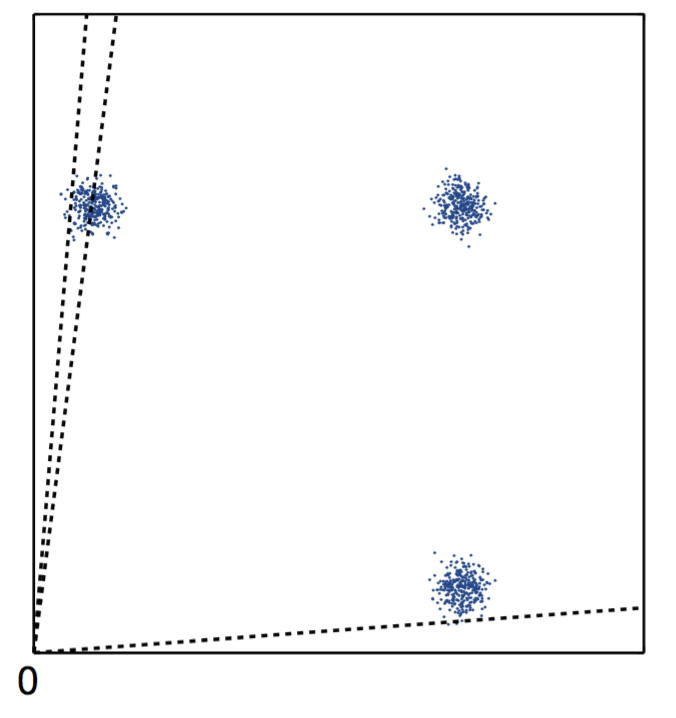
\includegraphics[width=\textwidth]{img/bvdVsOnmtf1.png}
        \caption{}
        \label{fig:bvdvsonmtf:1}
    \end{subfigure}
    ~ %add desired spacing between images, e. g. ~, \quad, \qquad, \hfill etc.
      %(or a blank line to force the subfigure onto a new line)
    \begin{subfigure}[b]{0.35\textwidth}
        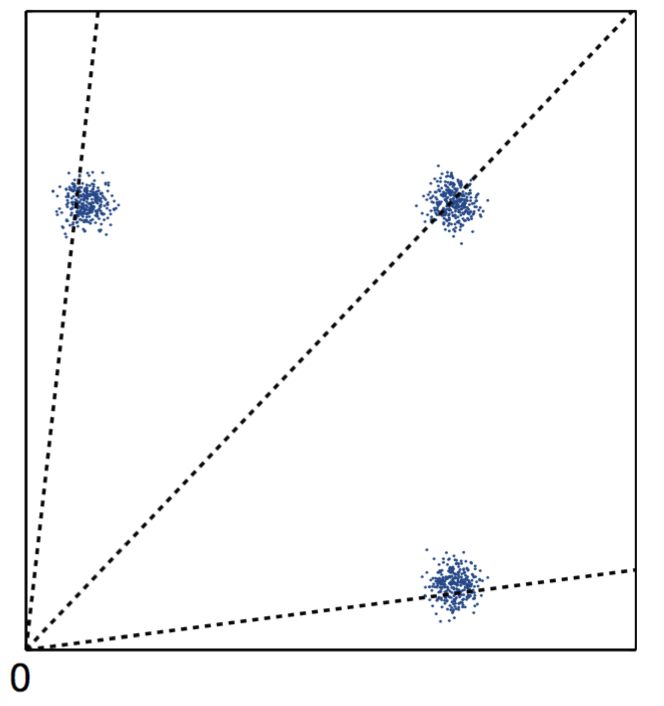
\includegraphics[width=\textwidth]{img/bvdVsOnmtf2.png}
        \caption{}
        \label{fig:bvdvsonmtf:2}
    \end{subfigure}
    \caption{
        Um exemplo sintético que compara o algoritmo para BVD contra o algoritmo para ONMTF, com pontos sendo dados, as linhas pontilhadas sendo os protótipos de linhas ($S V^T$), e os três conjuntos de pontos sendo os grupos.
        (a) O algoritmo para BVD encontra uma solução com dois protótipos em um mesmo grupo, deixando um dos grupos sem nenhum protótipo para representá-lo.
        Apesar de ser uma solução correta, ou seja, encontra um mínimo local, não é a desejada.
        (b) O algoritmo para ONMTF é capaz de encontrar a solução em que cada protótipo aproxima cada grupo de dados, através das restrições referentes à ortogonalidade, este é capaz de restringir as possíveis soluções para a fatoração $X \approx U S V^T$.
        \cite{Yoo2010}
    }
    \label{fig:bvdvsonmtf}
\end{figure}

\begin{problem}[Problema de Fatoração Ortogonal tripla de Matrizes Não-negativas]
\label{def:onmtf:problem}
\begin{equation}
    \begin{array}{lclcl}
        \displaystyle \mathcal{F}_2(U, S, V) & = & \displaystyle \min_{U, S, V} & \norm{X - USV^T}^{2}_{F}      \\
                                             &   & \text{suj. a}                & U \geq 0, S \geq 0, V \geq 0, \\
                                             &   &                              & U^T U = I,                    \\
                                             &   &                              & V^T V = I
    \end{array}
\end{equation}
\end{problem}

onde $U \in \mathbb{R}^{n \times k}_{+}$, $S \in \mathbb{R}^{k \times l}_{+}$, $V \in \mathbb{R}^{m \times l}$, $U \geq 0, S \geq 0, V \geq 0$ sendo todos os elementos de $U$, $S$ e $V$, maior que $0$, respectivamente, $U^T U = I$ e $V^T V = I$ as restrições de ortonomalidade para as matrizes indicadoras de grupos de linhas e colunas, respectivamente, e $\norm{\cdot}_F$ denota a norma de Frobenius para matrizes.

\citeonline{Ding06} propõem uma solução semelhante ao que foi apresentado na subseção~\ref{subsec:bvd}, fazendo a derivação através da função lagrangeana e a introdução dos multiplicadores de lagrange, utilizando as condições de otimização não-linear de KKT, derivando as regras para atualização multiplicativa para $U$, $S$ e $V$, apresentadas no algoritmo~\ref{algo:onmtf}.
Considere $t$ o contador de iterações, e $U^{(t)}$, $S^{(t+1)}$ e $V^{(t+1)}$, as matrizes $U$, $S$ e $V$, na iteração $t$, respectivamente.

\begin{algorithm}
\caption{Algoritmo baseado em atualização multiplicativa para solução do ONMTF}
\label{algo:onmtf}
    \begin{algorithmic}[1]
        \Function{ONMTF}{$X$, $maxIter$}
            \State \textbf{Inicialize:} $U^{(0)} \geq 0, V^{(0)} \geq 0, S^{(0)} \geq 0$ e $t \gets 0$.
            \While{(não convergiu) ou ($t \leq maxIter$)} %\Comment{We have the answer if r is 0}
                \State
                    \begin{equation}
                    \label{eq:onmtf:updateU}
                        U^{(t+1)} \gets U^{(t)} \odot \frac{ X V^{(t)} S^{(t)^T} }{ U^{(t)} U^{(t)^T} X V^{(t)} S^{(t)^T} }
                    \end{equation}
                \State
                    \begin{equation}
                    \label{eq:onmtf:updateV}
                        V^{(t+1)} \gets V^{(t)} \odot \frac{ X^T U^{(t+1)} S }{ V^{(t)} V^{(t)^T} X^T U^{(t+1)} S^{(t)} }
                    \end{equation}
                \State
                    \begin{equation}
                    \label{eq:onmtf:updateS}
                        S^{(t+1)} \gets S^{(t)} \odot \frac{ U^{(t+1)^T} X V^{(t+1)} }{ U^{(t+1)^T} U^{(t+1)} S^{(t)} V^{(t+1)^T} V^{(t+1)} }
                    \end{equation}
                \State $t \gets t + 1$
            \EndWhile\label{euclidendwhile}
            \State \textbf{return} $U^{(t+1)}, S^{(t+1)}, V^{(t+1)}$
        \EndFunction
    \end{algorithmic}
\end{algorithm}

No artigo de \citeonline{Yoo2010}, é proposta uma abordagem mais simples para a derivação das regras de atualização multiplicaticas, considere uma função de otimização qualquer $\mathcal{J}$ e seu respectivo gradiente $\nabla \mathcal{J}$:

\[
    \begin{array}{lclcl}
        \nabla \mathcal{J} & = & [\nabla \mathcal{J}]^+ - [\nabla \mathcal{J}]^-
    \end{array}
\]

onde $[\nabla \mathcal{J}]^+$ é a parte positiva do gradiente, $[\nabla \mathcal{J}]^-$ a parte negativa do gradiente.
Se $[\nabla \mathcal{J}]^+ \geq 0$ e $[\nabla \mathcal{J}]^- \geq 0$, então, é possível definir uma regra de atualização multiplicativa, para otimizar os parâmetros $\Theta$ da função $\mathcal{J}$:

\begin{equation}
\label{eq:onmtf:updateTheta}
    \Theta \gets \Theta \odot \left ( \frac{ [\nabla \mathcal{J}]^- }{ [\nabla \mathcal{J}]^+ } \right )^{\cdot \eta}
\end{equation}

onde $\odot$ representa o produto Hadamard, $(\cdot)^{\cdot \eta}$ representa a potência para cada elemento, e $\eta$ uma taxa de aprendizado ($0 < \eta \leq 1$).
Então, se $\Theta$ for inicializado com elementos positivos, é possível verificar que a regra de atualização multiplicativa da equação~\ref{eq:onmtf:updateTheta} mantém a não-negatividade de $\Theta$.

Também, é utilizada uma abordagem diferente para a derivação de regras de atualização multiplicativas, visando um algoritmo para a solução do problema~\ref{def:onmtf:problem}.
Neste caso, o gradiente é calculado com base em uma superfície com restrições que preserva a ortogonalidade.
Essa superfície com restrições é chamada de Variedade de Stiefel (\textit{Stiefel Manifold}), neste caso é usada a Variedade de Stiefel no espaço euclidiano, denotada por $\mathcal{H}_{a,b}$, sendo essa variedade o conjunto de $a \times b$ matrizes ortonormais no espaço $\mathbb{R}^a$, formalmente:

\[
    \begin{array}{lclcl}
        \mathcal{H}_{a, b} & = & \{ Y \in \mathbb{R}^{a \times b}: Y^T Y = I \}
    \end{array}
\]

Note que quando $b = 1$, a superfície se torna uma esfera.
Para otimização, considerando que essa esfera sejam as restrições do problema, o ideal é propor métodos que permanecam na esfera, então, todos os vetores tangentes à essa esfera, podem ser direções possíveis para um algoritmo de otimização iterativo, como mostra a Figura~\ref{fig:stiefel}.

\begin{figure}[H]
\centering
    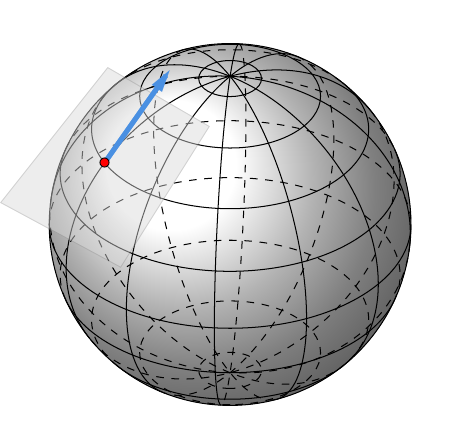
\includegraphics[width=0.3\textwidth]{img/stiefel.png}
    \caption{
        Uma Variedade Stiefel no espaço Euclidiano, que quando $b = 1$ essa superfície será uma esfera, e um dos possíveis vetores que está contido no conjunto dessa variedade (tangente à esfera).
    }
    \label{fig:stiefel}
\end{figure}

\citeonline{Edelman1999} definem o gradiente em um ponto $Y$, com a restrição $Y^T Y = I$, de uma função $\mathcal{J}$ definida em uma Variedade Stiefel no espaço euclidiano como:

\begin{equation}
\label{eq:stiefeldiff}
    \begin{array}{lclcl}
        {\tilde \nabla}_Y \mathcal{J} & = & \nabla_Y \mathcal{J} - Y (\nabla_Y \mathcal{J})^T Y
    \end{array}
\end{equation}

onde $\nabla_Y \mathcal{J}$ é o gradiente da função $\mathcal{J}$ para todos os elementos da matriz $Y$.

Dada a equação~\ref{eq:stiefeldiff}, \citeonline{Yoo2010} propõem os seguintes cálculos dos gradientes em Variedades Stiefel para $\mathcal{F}_2$, com $U$ no conjunto $\{ U^T U = I \}$, e com $V$ no conjunto $\{ V^T V = I \}$:

\[
    \begin{array}{lclclclcl}
        {\tilde \nabla_U} \mathcal{F}_2 & = & \nabla_U \mathcal{F}_2 - U (\nabla_U \mathcal{F}_2)^T U & = & U S V^T X^T U - X V S^T \\
        {\tilde \nabla_V} \mathcal{F}_2 & = & \nabla_V \mathcal{F}_2 - V (\nabla_V \mathcal{F}_2)^T V & = & V S^T U^T X V - X^T U S
    \end{array}
\]

Restando apenas o cálculo do gradiente para $S$, que como não há restrições, será igual à atualização do algoritmo para solução do BVD:

\[
    \begin{array}{lclcl}
        {\tilde \nabla_S} \mathcal{F}_2 & = & \nabla_S \mathcal{F}_2 & = & U^T U S V^T V - U^T X V
    \end{array}
\]

É possível, assim, usar a estratégia da equação~\ref{eq:onmtf:updateTheta} e os gradientes calculados, para propor uma solução para o problema de ONMTF, alternativas às atualizações das equações~\ref{eq:onmtf:updateU}, \ref{eq:onmtf:updateV} e~\ref{eq:onmtf:updateS}, através da atualização multiplicativa.
Essas atualizações são apresentadas nas equações~\ref{eq:onmtf2:updateU}, ~\ref{eq:onmtf2:updateV} e~\ref{eq:onmtf2:updateS}.

\begin{subequations}
    \begin{alignat}{2}
        U^{(t+1)} \gets \quad && U^{(t)} \odot \frac{ X V^{(t)} S^{(t)^T} }{ U^{(t)} S^{(t)} V^{(t)^T} X^T U^{(t)} }                   \label{eq:onmtf2:updateU} \\
        V^{(t+1)} \gets \quad && U^{(t)} \odot \frac{ X^T U^{(t+1)} S^{(t)} }{ V^{(t)} S^{(t)^T} U^{(t+1)^T} X V^{(t)} }               \label{eq:onmtf2:updateV} \\
        S^{(t+1)} \gets \quad && S^{(t)} \odot \frac{ U^{(t+1)^T} X V^{(t+1)} }{ U^{(t+1)^T} U^{(t+1)} S^{(t)} V^{(t+1)^T} V^{(t+1)} } \label{eq:onmtf2:updateS}
    \end{alignat}
\end{subequations}

% TODO: Falar do algoritmo que considera probabilidades

\section{Fatoração tripla rápida de Matrizes Não-negativas}

O problema de Fatoração tripla rápida de Matrizes Não-negativas (\textit{Fast Non-negative Matrix Tri Factorization} - FNMTF) foi proposto por \citeonline{Wang2011}, com os seguintes argumentos contra o uso prático dos problemas até agora propostos para encontrar cogrupos: os problemas de fatoração em três matrizes propostos até o momento, envolviam soluções algorítmicas iterativas, com multiplicações de matrizes intensas em cada etapa; e pelo fato dos algoritmos propostos realizarem coagrupamento relaxado, necessitando de pós-processamento para a extração dos grupos, o que implica em inúmeras soluções para o agrupamento.

\begin{problem}[Fatoração tripla rápida de Matrizes Não-negativas]
\label{def:fnmtf:problem}
\begin{equation}
    \begin{array}{lclcl}
        \displaystyle \mathcal{F}_3(F, S, G) & = & \displaystyle \min_{F, S, G} & \norm{X - FSG^T}^{2}_{F} \\
                                             &   &                              & F \in \Psi^{n \times k}, \\
                                             &   &                              & G \in \Psi^{m \times l}
    \end{array}
\end{equation}
\end{problem}

onde $X \in \mathbb{R}^{n \times m}$, $S \in \mathbb{R}^{k \times l}$, $\Psi = \{0, 1\}$.

Assim como nos outros algoritmos, $F$ é uma matriz indicadora dos grupos de linhas, $G$ uma matriz indicadora dos grupos de colunas, e $S$ contém os fatores que conectam um grupo de linhas aos grupos de colunas, e, um grupo de colunas aos grupos de linhas.

Como não há restrições em $\mathcal{F}_3$, é possível encontrar uma regra de atualização para $S$, e portanto, minimização de $\mathcal{F}_3$:
\[
    \begin{array}{lclcl}
        \nabla_S \mathcal{L} &     =    & F^T X G - F^T F S G^T G                 & = & 0                                 \\
                             & \implies & F^TFSG^TG                               & = & F^TXG                             \\
                             & \implies & (F^T F)^{-1} F^T F S G^T G (G^T G)^{-1} & = & (F^T F)^{-1} F^T X G (G^T G)^{-1}
    \end{array}
\]

\begin{equation}
\label{eq:fnmtf:updateS}
    \begin{array}{lclcl}
        \therefore & S & = & (F^T F)^{-1} F^T X G (G^T G)^{-1}
    \end{array}
\end{equation}

Sendo assim, é possível resolver os subproblema para atualizar $F$ e $G$.
Primeiramente, fixando $S$ e $G$ e resolvendo o problema~\ref{def:fnmtf:problem} para $F$ de forma iterativa, verificando para cada linha de $X$, qual o protótipo mais o aproxima (semelhante ao algoritmo de agrupamento \textit{K-means}), da mesma forma, é possível fixar $S$ e $F$ para alcançar uma solução iterativa para $G$, assim como mostra o algoritmo~\ref{algo:fnmtf}.
Considere os índices $i = \{1, \dots, n\}$, $j = \{1, \dots, m\}$, $p = p' = \{1, \dots, k\}$, e $q = q' = \{1, \dots, l\}$, o contador de iterações $t$, e $U^{(t)}$, $S^{(t+1)}$ e $V^{(t+1)}$, as matrizes $U$, $S$ e $V$, na iteração $t$, respectivamente.

\begin{algorithm}
\caption{Algoritmo FNMTF}
\label{algo:fnmtf}
    \begin{algorithmic}[1]
        \Function{FNMTF}{$X$, $maxIter$}
            \State \textbf{Inicialize:} $F^{(0)} \geq 0, S^{(0)} \geq 0, G^{(0)} \geq 0$ e $t \gets 0$.
            \While{(não convergiu) ou ($t \leq maxIter$)}
                \State
                    \begin{equation}
                    \label{eq:fnmtf:updateS}
                        S^{(t+1)} \gets (F^{(t)^T} F^{(t)})^{-1} F^{(t)^T} X G^{(t)} (G^{(t)^T} G^{(t)})^{-1}
                    \end{equation}
                \State
                    \[
                        {\tilde g}_{pj} \gets (S^{(t+1)} G^{(t)^T})_{pj}, \forall p, j
                    \]
                \State
                    \begin{equation}
                    \label{eq:fnmtf:updateF}
                        (F^{(t+1)})_{ip} \gets \left\{
                            \begin{array}{ll}
                                1 & p = \argmin_{p' \in \{1, \dots, k\}} \norm{ x_{i \cdot} - {\tilde g}_{p' \cdot} }^2 \\
                                0 & \textit{caso contrário}
                            \end{array}
                        \right. \forall i, p
                    \end{equation}
                \State
                    \[
                        {\tilde f}_{iq} \gets (F^{(t+1)} S^{(t+1)})_{iq}, \forall i, q
                    \]
                \State
                    \begin{equation}
                    \label{eq:fnmtf:updateG}
                        (G^{(t+1)})_{jq} \gets \left\{
                            \begin{array}{ll}
                                1 & q = \argmin_{q' \in \{1, \dots, l\}} \norm{ x_{\cdot j} - {\tilde f}_{\cdot q'} }^2 \\
                                0 & \textit{caso contrário}
                            \end{array}
                        \right. \forall j, q
                    \end{equation}
                \State $t \gets t + 1$
            \EndWhile\label{euclidendwhile}
            \State \textbf{return} $F^{(t+1)}, S^{(t+1)}, G^{(t+1)}$
        \EndFunction
    \end{algorithmic}
\end{algorithm}

% ************************************************************
% ************************************************************
% ************************************************************

\chapter{Algoritmos propostos}
\label{ch:proposedalgs}

\section{Fatoração Tripla de Matrizes Não-negativas Sobrepostas}

\begin{problem}[Problema de Fatoração Tripla de Matrizes Não-negativas Sobrepostas]
\label{def:ovnmtf:problem}
\begin{equation}
    \begin{array}{lclc}
        \displaystyle \mathcal{F}_4(U, S, V_{(1)}, \dots, V_{(k)}) & = & \displaystyle \min_{U, S, V_{(1)}, \dots, V_{(k)}} & \norm{X - U\sum_{p=1}^{k}I_{(p)}SV_{(p)}^T}^{2}_{F} \\
                                                                   &   & \text{suj. a}                & U \geq 0, \\
                                                                   &   &                              & S \geq 0, \\
                                                                   &   &                              & V_{(p)} \geq 0, \quad \forall p
    \end{array}
\end{equation}
\end{problem}

sendo os índices $p = \{1, \dots, k\}$, o conjunto de matrizes $\mathcal{V} = \{ V_{(1)}, \dots, V_{(k)} \}$, em que cada $V_{(p)} \in \mathbb{R}^{m \times l}_{+}$, uma matriz seletora $I_{(p)}$ que contém $1$ na posição $I_{p,p}$ da sua diagonal e $0$ no resto, $U \in \mathbb{R}^{n \times k}_{+}$, $S \in \mathbb{R}^{k \times l}_{+}$, e $\norm{\cdot}_F$ a norma de Frobenius para matrizes.

\begin{algorithm}
\caption{Algoritmo baseado em atualização multiplicativa para solução do OvNMTF}
\label{algo:ovnmtf}
    \begin{algorithmic}[1]
        \Function{OvNMTF}{$X$, $maxIter$}
            \State \textbf{Inicialize:} $U^{(0)} \geq 0, S^{(0)} \geq 0, V_{(0)}^{(0)} \geq 0, \dots, V_{(k)}^{(0)} \geq 0$ e $t \gets 0$.
            \While{(não convergiu) ou ($t \leq maxIter$)} %\Comment{We have the answer if r is 0}
                \State
                    \begin{equation}
                    \label{eq:ovnmtf:updateU}
                        U^{(t+1)} \gets U^{(t)} \odot \sum_{p=1}^{k} \frac{ X V^{(t)^T}_{(p)} S^{(t)^T} I_{(p)} }{ \sum_{p'=1}^k U^{(t)} I_{(p)} S^{(t)} V^{(t)}_{(p)} V^{(t)^T}_{(p')} S^{(t)^T} I_{(p')} }
                    \end{equation}
                \For{$p \leftarrow 1, k$}
                    \State
                        \begin{equation}
                        \label{eq:ovnmtf:updateV}
                            V^{(t+1)}_{(p)} \gets V^{(t)}_{(p)} \odot \frac{ S^{(t)^T} I_{(p)} U^{(t+1)^T} X }{ S^{(t)^T} I_{(p)} U^{(t+1)^T} U^{(t+1)} I_{(p)} S^{(t)} V^{(t)}_{(p)} }
                        \end{equation}
                \EndFor
                \State
                    \begin{equation}
                    \label{eq:ovnmtf:updateS}
                        S^{(t+1)} \gets S^{(t)} \odot \sum_{p=1}^{l} \frac{ I_{(p)} U^{(t+1)^T} X V^{(t+1)^T}_{(p)} }{ \sum_{p'=1}^{l} I_{p} U^{(t+1)^T} U^{(t+1)} I_{(p')} S^{(t)} V^{(t+1)}_{(p')} V^{(t+1)^T}_{(p)} }
                    \end{equation}
                \State $t \gets t + 1$
            \EndWhile\label{euclidendwhile}
            \State \textbf{return} $U^{(t+1)}, S^{(t+1)}, V_{(1)}^{(t+1)}, \dots, V_{(k)}^{(t+1)}$
        \EndFunction
    \end{algorithmic}
\end{algorithm}


\section{Fatoração Binária Tripla de Matrizes Não-negativas Sobrepostas}

\begin{problem}[Problema de Fatoração Binária Tripla de Matrizes Não-negativas Sobrepostas]
\label{def:binovnmtf:problem}
\begin{equation}
    \begin{array}{lclc}
        \displaystyle \mathcal{F}_5(F, S, G_{(1)}, \dots, G_{(k)}) & = & \displaystyle \min_{F, S, G_{(1)}, \dots, G_{(k)}} & \norm{ X - F \sum_{p=1}^{k} I_{(p)} S G_{(p)}^T }^{2}_{F} \\
                                                                   &   & \text{suj. a}                & F \in \Psi^{n \times k}, \\
                                                                   &   &                              & S \in \Psi^{k \times l}, \\
                                                                   &   &                              & G_{(p)} \in \Psi^{m \times l}, \quad \forall p
    \end{array}
\end{equation}
\end{problem}

sendo $\Psi = {0, 1}$, os índices $p = \{1, \dots, k\}$, o conjunto de matrizes $\mathcal{G} = \{ G_{(1)}, \dots, G_{(k)} \}$, uma matriz seletora $I_{(p)}$ que contém $1$ na posição $I_{p,p}$ da sua diagonal e $0$ no resto, $S \in \mathbb{R}^{k \times l}_{+}$, $X \in \mathbb{R}^{n \times m}_{+}$, e $\norm{\cdot}_F$ a norma de Frobenius para matrizes.

\begin{algorithm}
\caption{Algoritmo BinOvNMTF}
\label{algo:binovbnmtf}
    \begin{algorithmic}[1]
        \Function{BinOvNMTF}{$X$, $maxIter$}
            \State \textbf{Inicialize:} $F^{(0)} \geq 0, S^{(0)} \geq 0, G_{(0)}^{(0)} \geq 0, \dots, G_{(k)}^{(0)} \geq 0$ e $t \gets 0$.
            \While{(não convergiu) ou ($t \leq maxIter$)}
                \State
                    \begin{equation}
                    \label{eq:binovbnmtf:updateS}
                        (S^{(t+1)})_{p q} \gets \frac{1}{\abs{\{\mathbf{x}_{i \cdot} \in \mathcal{C}_p\}} \abs{\{\mathbf{x}_{\cdot j} \in \mathcal{W}_q\}}} \sum_{i = 1}^{n} \sum_{j = 1}^{m} \sum_{\mathbf{x}_{i \cdot} \in \mathcal{C}_p} \sum_{\mathbf{x}_{\cdot j} \in \mathcal{W}_q} x_{i j}
                    \end{equation}
                \For{$p \leftarrow 1, k$}
                \State
                    \[
                        {\tilde F} \gets
                            \begin{bmatrix}
                                         & \vdots                                                                     &          \\
                                \horzbar & \mathbf{f}_{i \cdot}^{(t)}, \forall \mathbf{x}_{i \cdot} \in \mathcal{C}_p & \horzbar \\
                                         & \vdots                                                                     &
                            \end{bmatrix} S^{(t+1)}
                    \]
                \State
                    \[
                        {\tilde X} \gets
                            \begin{bmatrix}
                                         & \vdots                                                                     &          \\
                                \horzbar & \mathbf{x}_{i \cdot}, \forall \mathbf{x}_{i \cdot} \in \mathcal{C}_p & \horzbar \\
                                         & \vdots                                                                     &
                            \end{bmatrix}
                    \]
                \State
                    \begin{equation}
                    \label{eq:binovbnmtf:updateG}
                        (G_{(p)}^{(t+1)})_{jq} \gets \left\{
                            \begin{array}{ll}
                                1 & q = \argmin_{q' \in \{1, \dots, l\}} \norm{ \mathbf{{\tilde x}}_{\cdot j} - \mathbf{{\tilde f}}_{\cdot q'} }^2 \\
                                0 & \textit{caso contrário}
                            \end{array}
                        \right. \forall j, q
                    \end{equation}
                \EndFor
                \State
                    \[
                        \mathbf{{\tilde g}}_{p \cdot} \gets (\mathbf{s}_{p \cdot}^{(t+1)} G_{(p)}^{(t)^T})_{pj}, \forall p
                    \]
                \State
                    \begin{equation}
                    \label{eq:binovbnmtf:updateF}
                        (F^{(t+1)})_{ip} \gets \left\{
                            \begin{array}{ll}
                                1 & p = \argmin_{p' \in \{1, \dots, k\}} \norm{ \mathbf{x}_{i \cdot} - \mathbf{{\tilde g}}_{p' \cdot} }^2 \\
                                0 & \textit{caso contrário}
                            \end{array}
                        \right. \forall i, p
                    \end{equation}
                \State $t \gets t + 1$
            \EndWhile\label{euclidendwhile}
            \State \textbf{return} $F^{(t+1)}, S^{(t+1)}, G_{(1)}^{(t+1)}, \dots, G_{(k)}^{(t+1)}$
        \EndFunction
    \end{algorithmic}
\end{algorithm}

% ************************************************************
% ************************************************************
% ************************************************************

% \chapter{A proposta}
% \label{ch:proposta}

% \section{Overlapping Orthogonal Nonnegative Matrix Tri Factorization}

% This is a proposal algorithm that aims to solve the following problem:
% $$\mathcal{F}_1 = \textit{min } ||X - U\sum_{i=1}^{k}I^{(i)}SV^{(i)}||^{2}_{F}$$
% % $$\textit{s.t. } U^TU = I$$
% % $$\left[ \begin{array}{c} V^{(1)} \\ V^{(2)} \\ \vdots \\ V^{(k)} \end{array} \right]^T\left[ \begin{array}{c} V^{(1)} \\ V^{(2)} \\ \vdots \\ V^{(k)} \end{array} \right] = I$$
% % $$\left[ \begin{array}{c} V^{(1)} \\ V^{(2)} \\ \vdots \\ V^{(k)} \end{array} \right] \geq 0$$
% $$\textit{s.t. } U, S, V^{(1)}, \dots, V^{(k)} \geq 0$$

% where $X \in \mathbb{R}^{n \times m}$ a data matrix, $U \in \mathbb{R}^{n \times k}$ an matrix containing rows clusters, $I^{(i)} \in \mathbb{R}^{k \times k}$ an indicator matrix, $S \in \mathbb{R}^{k \times l}$ a block matrix, $V^{(i)} \in \mathbb{R}^{l \times m} \forall i \in \{1, \dots, k\}$ matrices containing columns clusters for each row cluster, and $||\cdot||^2_{F}$ denotes the frobenius norm.


% Consider the lagrange function:
% $$\mathcal{L} = \mathcal{F}_1 - tr(\Lambda_1 U^T) - tr(\Lambda_2 S^T) - \sum_{i=1}^{k} tr(A_i V^{(i)^T})$$

% where $\Lambda_1, \Lambda_2$ and $A_i \forall i \in \{1, \dots, k\}$ are lagrange multipliers: $\Lambda_1 \in \mathbb{R}^{n \times k}$, $\Lambda_1 \in \mathbb{R}^{k \times l}$, and $A_i \in \mathbb{R}^{k \times l} \forall i \in \{1, \dots, k\}$.

% KKT Conditions:
% \begin{itemize}
% \item $\frac{\partial \mathcal{L}}{\partial U} = 0$
% \item $\frac{\partial \mathcal{L}}{\partial S} = 0$
% \item $\frac{\partial \mathcal{L}}{\partial V^{(i)}} = 0, \forall i \in \{1, \dots, k\}$
% \item $\Lambda_1 \odot U = 0$
% \item $\Lambda_2 \odot S = 0$
% \item $A_i \odot V^{(i)} = 0, \forall i \in \{1, \dots, k\}$
% \end{itemize}
% %\paragraph{}
% where $\odot$ denotes the element-wise multiplication.

% Given that:
% $$\frac{\partial}{\partial B} tr \left[ (RBC + D)(RBC + D)^T \right] = 2R^T(RBC + D)C^T = 2R^trBCC^T + 2R^TDC^T$$

% It is possible to calculate $\frac{\partial \mathcal{L}}{\partial U}$, considering $R = -I, B = U, C = \sum I^{(i)}SV^{(i)}, D = X$:
% $$\frac{\partial \mathcal{L}}{\partial U} = 2 U \sum_{i=1}^k I^{(i)} S V^{(i)} \sum_{j=1}^k V^{(j)^T} S^T I^{(j)} - 2 X \sum_{i=1}^k V^{(i)^T} S^T I^{(i)} - \Lambda_1$$

% For $\frac{\partial \mathcal{L}}{\partial V}$, consider $R = U \sum I^{(i)} S, B = V^{(i)}, C = -I, D = X$:
% $$\frac{\partial \mathcal{L}}{\partial V^{(j)}} = 2 S^T I^{(j)} U^T U I^{(j)} S V^{(j)} - 2 S^T I^{(j)}  U^T X - A_j, \forall j \in \{1, \dots, k\}$$

% For $\frac{\partial \mathcal{L}}{\partial S}$, consider that $\frac{\partial (A X B X^T C)}{\partial X} = A^T C^T X B^T + C A X B$:
% $$\frac{\partial \mathcal{L}}{\partial S} = \frac{\partial}{\partial S} tr (X - U \sum_{i=1}^{k} I^{(i)} S V^{(i)}) (U \sum_{j=1}^{k} I^{(j)} S V^{(j)})^T   - tr(\Lambda_2 S^T)$$

% $$= \frac{\partial}{\partial S} tr(X^TX) - 2 \frac{\partial}{\partial S} tr(X U \sum_{i=1}^{k} I^{(i)} S V^{(i)}) + tr(\sum_{j=1}^k \sum_{i=1}^k U I^{(i)} S V^{(i)} V^{(j)^T} S^T I^{(j)} U^T ) - tr(\Lambda_2 S^T)$$

% $$= -2 \sum_{i=1}^{k} I^{(i)} U^T X^T V^{(i)^T} + \sum_{i=1}^{k} \sum_{j=1}^{k} [ I^{(i)} U^T U I^{(j)} S V^{(j)} V^{(i)^T} +  I^{(j)} U^T U I^{(i)} S V^{(i)} V^{(j)^T} ]$$

% $$= -2 \sum_{i=1}^{k} I^{(i)} U^T X^T V^{(i)^T} + \sum_{i=1}^{k} \sum_{j=1}^{k} I^{(i)} U^T U I^{(j)} S V^{(j)} V^{(i)^T}$$


% ************************************************************
% ************************************************************
% ************************************************************

% \section{Prova de conceito - Sistemas de Recomendação}
% \label{sec:sr}

% A grande maioria das pessoas que usam a \textit{web} muito provavelmente já interagiu com algum Sistema de Recomendação (SR), e por isso, o conceito que define esse tipo de sistema é intuitivo. Porém, por ser uma área de estudo relativamente nova \cite{Lops2011}, diferentes autores usam definições diversas, visto que a interpretação do que consiste um SR difere dependendo do ponto de vista de cada autor \cite{Leino2014}.

% \citeonline{Resnick1997}, autores que criaram o termo Sistemas de Recomendação \cite{Neumann2007,Leino2014}, argumentam que SRs servem para ajudar em processos de tomada de decisão do dia-a-dia, como quais itens comprar, quais músicas ouvir, ou quais notícias ler.
% Além disso, \citeonline{Resnick1997} provê uma taxonomia na área de Sistemas de Recomendação:

% \begin{itemize}
%   \item Conteúdo recomendado: os itens que são recomendados pelo Sistema de Recomendação. Por exemplo: produtos, músicas, notícias e/ou etc.
%   \item Entrada dos usuários: as interações que os usuários realizam com os itens são a entrada para um SR, e elas podem ser implícitas (o usuário $u$ leu a notícia $I$) ou explícitas (o usuário $u$ classificou o filme $I$ como $5$ estrelas).
%   \item Alvo da recomendação: os itens podem ser recomendados especificamente para um usuário (personalizado), direcionados para um grupo de usuários ou a todos os usuários (não-personalizado).
%   \item Técnicas para recomendação (agregações): as estratégias e os algoritmos que os SRs usam para criar as recomendações.
%   \item Uso das recomendações: trata-se de como mostrar as recomendações para os usuários. Por exemplo: por meio do filtro de recomendações negativas, ordenando por um fator de classificação numérico, etc.
% \end{itemize}

% Porém, definições mais recentes \cite{Burke2002,Burke2007}, descrevem SRs como qualquer sistema que produz recomendações personalizadas ou tem o efeito de guiar um usuário de modo personalizado, mostrando itens que possam ser interessantes para ele, dentro de uma grande quantidade de opções.
% Isso faz com que SRs que provêm recomendações não-personalizadas deixem de se adequarem à definição de SR.
% % \textcolor{red}{Por outro lado, pode-se considerar que essa definição mais específica e a inadequação de alguns sistemas a ela ocorro porque ela está baseada nas estratégias para construção de SRs atualmente, ou mesmo na demanda pelo tipo de recomendação atual, que possuem o foco em produzir recomendações personalizadas.}
% %É provável que isso se deve ao fato que das estratégias usadas atualmente, que têm o foco de produzir recomendações personalizadas.

% Formalmente, \citeonline{Burke2002,Burke2007} define SRs como um conjunto de itens $\mathcal{I}$ que podem ser recomendados, um conjunto de usuários $U$ cujas preferências são conhecidas, um usuário $u$ pra o qual as recomendações são geradas, e algum item $i$ para o qual se quer predizer a preferência para $u$.
% \citeonline{Adomavicius2005} extendem a definição de SR com uma função de utilidade $f$ que mede o quão útil é o item $i$ para o usuário $u$: $f: \mathcal{I} \times U \rightarrow R$, em que $R = \{ r_{u_1,I_1}, \dots, r_{u_1,I_m}, \dots, r_{u_1,I_M}, \dots, r_{u_n,I_1}, \dots, r_{u_n,I_M}, \dots, r_{u_N,I_1}, \dots, r_{u_N,I_m}, \dots,\\ r_{u_N, I_M} \}$ é um conjunto ordenado com valores faltantes, sendo $r_{u_n,i_m}$ um inteiro ou real que representa a interação do usuário $u_n$ no item $i_m$.
% No entanto, existem tipos de SRs que não estimam $f$ completamente, podendo otimizar funções auxiliares para gerar as recomendações à um usuário $u$ \cite{Lops2011}.

% % Essa função de utilidade poderia ser usada na definição de serendipidade. Não vamos conseguir isso para agora, mas é preciso pensar nisso.

% Em síntese, um SR tem a função de auxiliar os usuários de uma aplicação a interagir com itens, provendo sugestões de com quais itens interagir, baseando-se no histórico de interações desses usuários com esses itens.

%  \subsection{Tipos de Sistemas de Recomendação}
%  \label{subsec:tipossr}

% Para estimar $f$ e chegar no conjunto ordenado $R$ existem diversas estratégias, e do uso delas surgem os tipos de SRs. Os tipos de SRs diferem quanto ao domínio, informações usadas para recomendação, e principalmente nas propriedades em que cada tipo se destaca.

% % Não sei se coloco a taxonomia tradicional, ou se coloco essa, handbook-1 diz que é clássica, podem burke de 2002 para 2007 muda a taxonomia, enquanto isso, Adomavicius usa a tradicional e o livro usa a tradicional + baseado em conhecimento

% % Vc deve escolher a taxonomia que mais lhe agrada e depois dela criar um parágrafo dizendo o que você disse no comentário acima, mas criando um texto melhor do que o usado no comentário. Um texto mais claro.

% \citeonline{Jannach2011} provêm uma taxonomia que categoriza os SRs em quatro diferentes tipos:
% \begin{itemize}
%  \item \textit{Filtragem colaborativa}, o primeiro tipo de SR que foi implementado \cite{Resnick1997}, tem como idéia básica encontrar outros usuários $u_{1,\dots,Z}$ em $U$, sendo $Z < N$ e não necessariamente em ordem, com preferências semelhantes à $u$, e então recomendar itens com os quais $u_{1,\dots,Z}$ interagiram e que $u$ ainda não interagiu, estabelecendo alguma métrica para estimar $f$. Medidas de similaridade geralmente usadas nesse contexto incluem \textit{Correlação de Pearson} e \textit{Similaridade dos Cossenos}. Também são usadas técnicas para redução de dimensionalidade como \textit{Decomposição de Valores Singulares} e \textit{Fatorização de Matriz} \cite{Jannach2011}.
%  \item \textit{Baseado em conteúdo}, é um dos tipos de SR que otimiza funções auxiliares à $f$. Descreve os itens por atributos que possibilitam o uso de medidas de similaridade entre itens. Então, com as interações dos usuários de $U$ e itens em $\mathcal{I}$, é construído um perfil de interesses para cada usuário. As recomendações são feitas a partir da combinação do perfil de interesses de um usuário $u$ com os itens em $\mathcal{I}$ que $u$ ainda não interagiu. Neste caso são usadas técnicas de Recuperação de Informação \cite{Jannach2011} para representar os itens e calcular similaridades entre itens, assim como técnicas de Aprendizado de Máquina supervisionado e não-supervisionado \cite{Jannach2011,Burke2002}.
%  \item \textit{Baseado em Conhecimento}, tem o intuito de sugerir itens de forma personalizada, baseando-se nas necessidades ou regras estabelecidas por um usuário $u$ e nas características dos itens em $\mathcal{I}$. São estabelecidas medidas de similaridade para estimar o quanto as necessidades do usuário são atendidas pelas recomendações \cite{Jannach2011,Lops2011,Burke2007}.
%  \item \textit{Híbrido}, é capaz de combinar as vantagens de cada tipo de SR para suprir as limitações associadas a cada um deles. A dificuldade, neste caso, está em como combinar as diferentes técnicas para recomendação \cite{Jannach2011,Burke2007}. \citeonline{Burke2007} identificou sete tipos de SRs Híbridos em uma revisão da literatura: \textit{Weighting}, atribui um peso para cada algoritmo a fim de ponderar as recomendações; \textit{Switching}, seleciona um dos algoritmos (ou tipos); \textit{Mixed}, recomendações são mostradas em conjunto; \textit{Combinação de características}, diferentes fontes são combinadas em apenas um algoritmo; \textit{Feature Augumentation}, uma técnica é usada para computar características que servem de entrada para outra técnica; \textit{Cascade}, é atribuído um grau de prioridade para cada algoritmo; \textit{Meta-level}, uma técnica gera um modelo, que é usado como entrada para outras técnicas.
% \end{itemize}

%  \subsubsection{Vantagens e desvantagens}
%  \label{subsubsec:lim}

% Cada um dos tipos de SRs descritos possuem algumas limitações.
% Em \citeonline{Jannach2011,Adomavicius2005,Burke2002,Lops2011} os problemas comuns encontrados no desenvolvimento de SRs são nomeados: \textit{novo usuário} (\textit{user cold-start}), \textit{novo item} (\textit{item cold-start}), \textit{esparsidade}, \textit{sobre-especialização} e \textit{análise de conteúdo limitada}.

% Os problemas de \textit{novo usuário} e \textit{novo item} são similares. Basicamente, enquanto o primeiro trata da dificuldade de gerar recomendações para novos usuários, o segundo trata de gerar recomendações para novos itens. O problema de \textit{novo usuário} esta presente como uma desvantagem nos SRs de filtragem colaborativa e baseado em conteúdo, pois o SR não conhece as preferências dos novos usuários, tendo dificuldade de construir um modelo que tenha como base essas preferências. Já o problema de \textit{novo item} é considerado uma vantagem para os SRs baseados em conteúdo, enquanto uma desvantagem para os SRs baseados em filtragem colaborativa. Como a filtragem colaborativa se baseia apenas nas interações de usuários e itens, um item novo, que não teve nenhuma ou teve poucas interações, não será recomendado. Diferentemente do SR baseado em conteúdo, que leva em consideração a representação do item para construir recomendações.

% Contrariamente, o problema de \textit{sobre-especialização} é uma vantagem para os SRs de filtragem colaborativa e uma desvantagem para os SRs baseados em conteúdo.
% A \textit{sobre-especialização} diz respeito ao problema de sugerir apenas itens previsíveis para o usuário, por exemplo, se o usuário viu notícias apenas de esporte, ele já espera receber sugestões de notícias de esporte, porém este usuário muito provavelmente pode gostar de ler notícias de outras categorias.
% A capacidade do SR de sugerir notícias imprevisíveis é chamado de serendipidade \cite{Jannach2011,Lops2011}.
% SRs baseados em conteúdo sofrem desse problema pois combinam o perfil de preferências de um usuário com os itens em $\mathcal{I}$, restrigindo o espaço de busca para realizar a sugestão de itens.
% Enquanto isso, os SRs baseados em filtragem colaborativa são capazes de oferecer sugestões úteis e serendipitas, pois são capazes de ampliar o espaço de busca através da estratégia de sugerir itens que usuários semelhantes à $u$ interagiram e que $u$ ainda não interagiu.

% Os SRs baseados em filtragem colaborativa são os únicos que sofrem do problema de \textit{esparsidade}, que é o fato de usuários interagirem com apenas um pequeno subconjunto do conjunto de itens, tornando a matriz de interações ou preferências ($U \times \mathcal{I}$) esparsa.
% Isso faz com que aumente a necessidade de ter uma grande quantidade de usuários, pois este tipo de SR necessita de intersecções nas interações de itens por usuários para que seja possível encontrar usuários similares a um dado usuário.

% Assim como os SRs de filtragem colaborativa, os SRs baseados em conteúdo sofrem de um problema único, que é a \textit{análise de conteúdo limitada}.
% Este problema se refere à representação dos itens, a qual precisa ser suficiente para discriminá-los \cite{Lops2011}.
% Em SRs baseados em conteúdo é comum haver a necessidade de limitar a representação de itens, tanto pelo número de atributos quanto pelo conteúdo que essas podem representar.
% Por exemplo, no contexto de notícias na \textit{web}, se a representação for um vetor com o número de ocorrências de cada palavra, perde-se a relação entre as palavras, e também todo o conteúdo que não é texto, como imagens, vídeos, etc.

%  \subsection{Avaliação da Recomendação}
%  \label{subsec:evalsr}

% Diferentes tipos de SRs foram discutidos juntamente com uma variedade de problemas relacionados a eles.
% Nesse contexto, faz-se a importância da discussão de como avaliar se uma estratégia adotada no desenvolvimento de um SR realmente é efetiva.
% SRs podem ser avaliados através de \textit{experimentos online}, que podem descobrir a real influência do SR no comportamento do usuário, e \textit{experimentos offline}, que estimam o erro de predição e simulam o comportamento do usuário no SR usando um conjunto de dados \cite{Ricci22011}.

% Para experimentos \textit{online} podem ser estabelecidas variáveis através da captura implícita ou explícita do comportamento, como satisfação do usuário e taxa de cliques (\textit{click-through rate} - CTR).
% Uma das maneiras para realizar esse tipo de experimento é por meio de testes A/B \cite{Jannach2011}, em que cada usuário, ao interagir com o SR, recebe um tratamento diferente aleatoriamente, dentro dos possíveis tratamentos estabelecidos pelo experimento.
% Assim, é possível dizer, por exemplo, a influência de um novo componente no SR no comportamento dos usuários.

% Tradicionalmente, SRs são avaliados através de experimentos \textit{offline} \cite{Jannach2011}.
% Por serem mais simples, esses tipos de experimentos podem ser usados, por exemplo, para selecionar os melhores algoritmos a serem aplicados no desenvolvimento de um SR. No entanto, \citeonline{Ricci22011} argumentam que não é possível medir diretamente a influência das recomendações no comportamento dos usuários.
% Para simular o comportamento do usuário em um SR usando um conjunto de dados, são estabelecidos dois subconjunto das interações de $u$ aleatoriamente ($\{ r_{u,i_4}, r_{u,i_3}, \dots \}$), um para treinamento dos modelos $\text{conj\_treino}_u$ e outro para teste $\text{conj\_teste}_u$.
% Assim é possível adotar estratégias semelhantemente àquelas adotadas em Aprendizado de Máquina, como avaliação da \textit{matriz de confusão} e de medidas derivadas como \textit{precisão}, \textit{revocação}, \textit{f1-score}, \textit{cross-validation} e etc.

% Na realidade, a estratégia de avaliação via \textit{matriz de confusão} pode ser usada em  \textit{experimentos online} e \textit{offline}, da seguinte maneira: se o usuário gostar do item sugerido à ele, é considerada uma predição correta (verdadeiro positivo); se o usuário não solicita preferência pela sugestão ou se não existe informações da preferência do usuário para esta sugestão, a predição é considerada errada (falso positivo); contrariamente, se o SR não fizer essas sugestões, é considerada uma emissão correta (verdadeiro negativo); por fim, se o SR não sugerir itens que o usuário tem preferência, é considerada uma predição errada (falso negativo).

% Uma das métricas mais comuns usadas para \textit{experimentos offline} é o \textit{erro absoluto médio} (\textit{Mean Absolute Error} - MAE) e \textit{raiz do erro quadrático médio} (\textit{Root Mean Squared Error} - RMSE) \cite{Jannach2011}\footnote{Essa métrica foi a utilizada na competição Netflix Prize (\textit{http://www.netflixprize.com/}), que teve grande repercursão na academia e na indústria}. A definição formal das métricas MAE e RMSE são descritas nas equações~\ref{eq:mae} e~\ref{eq:rmse}, respectivamente.

% \begin{equation}
% \label{eq:mae}
% MAE = \sum_{u \in U} \frac{\sum_{i \in \text{conj\_teste}_u} |f(u,i) - r_{u,i}|}{|\text{conj\_teste}_u|}
% \end{equation}

% \begin{equation}
% \label{eq:rmse}
% RMSE = \sum_{u \in U} \sqrt{\frac{\sum_{i \in \text{conj\_teste}_u} (f(u,i) - r_{u,i}^2)}{|\text{conj\_teste}_u|}}
% \end{equation}

% A métrica MAE computa o erro médio entre as predições feitas pelo SR ($f(u,i)$) e os valores reais das preferências dos usuários ($r_{u,i}$) para todos os usuários em $U$, enquanto o RMSE amplifica erros grandes, pois eleva o mesmo ao quadrado. Essas métricas são usadas para valores reais, ou seja, $r_{u,i} \in [0,1]$, por exemplo.

% Para valores binários de $r_{u,i}$, ou quando deseja-se prever o número de recomendações relevantes para um usuário $u$, são usadas as métricas \textit{precisão} e \textit{revocação} \cite{Jannach2011}.

% Para medir a serendipidade das recomendações, \citeonline{Ricci22011} propõem uma estratégia: estabelecer uma medida de distância entre itens e rotular os itens com menor distância entre si como ausentes de serendipidade, assim, algoritmos que evitem esses itens, serão considerados superiores.

% % acho que você pode citar esse autor na metodologia dizendo que ele apresenta uma métrica a ser usada para avaliar sua modelagem. Com isso vc vai dando um pouco mais de força para a sua metodologia.


%    \subsection{Essembles para clusterização}
% ************************************************************
% ************************************************************
% ************************************************************


\chapter{Experimentos e Resultados}
\label{ch:experiments}

% TODO onde falar sobre validação de cluster \section{Validação de clusters?}

Para fim de validação dos algoritmos foram feitos experimentos utilizando bases de dados sintéticas, base de dados toy e base de dados reais.
% experimentos foram feitos para verificar que os algoritmos desenvolvidos são úteis para descobrir estrutura com intersecção, provendo evidências que suportam o objetivo principal deste trabalho
Estes experimentos foram realizados à fim de comprovar a utilidade de métodos de Cocluterização baseados em Fatoração de Matrizes, tanto os algoritmos desenvolvidos quanto os já presentes na literatura, para coclusterização de documentos e mineração destes documentos.
Os algoritmos usados nos experimentos compõem algoritmos de clustering tradicionais: \textit{k-means} e \textit{fuzzy k-means}, e algoritmos de coclustering baseados em fatoração de matrizes da literatura: \textit{ONMTF}, \textit{FNMTF}; e os algoritmos propostos no capítulo~\ref{ch:proposedalgs}: \textit{OvNMTF} e \textit{BinOvNMTF}.

\section{Experimentos com Base de Dados sintéticas}

As bases de dados sintéticas foram criadas com inspiração nas diferentes estruturas de biclusters, propostas por \citeonline{Madeira2004}.

\begin{figure}[H]
\centering
    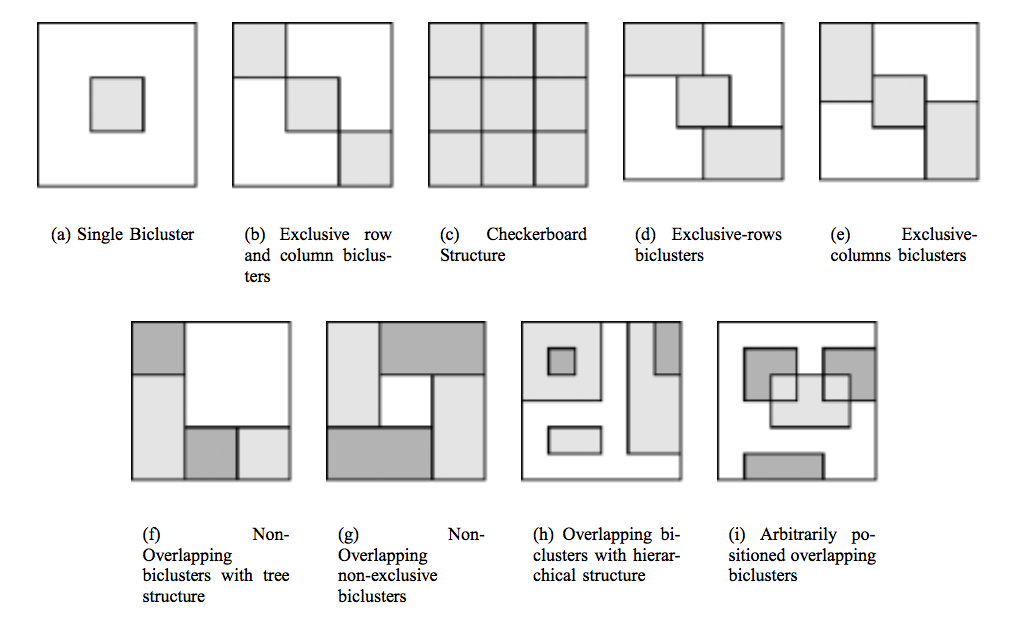
\includegraphics[width=0.7\textwidth]{img/synteticBiclusters.png}
    \caption{
        Tipos diferentes de biclusters.
    }
    \label{fig:biclusters-structures}
\end{figure}

A forma de interpretar as matrizes da figura~\ref{fig:biclusters-structures} é considerar cada elemento dessa matriz como uma cor relacionada com o seu valor, organizando as linhas e colunas, de tal forma que os valores similares formem retângulos, que são os biclusters.

Cada bicluster foi gerado a partir de valores centrais de um conjunto de valores centrais $C = \{ 20, 40, 60, 80, 100, 120, 140, 160, 180 \}$, sendo assim, é escolhido um valor central $c \in C$ de forma aleatória e adicionado valores de $0$ à $10$, gerados a partir de uma distribuição uniforme, para formar um bicluster.
Então, um os valores de um bicluster $B$, que é uma submatriz dos dados originais, é gerado pela equação~\ref{eq:genbic}.

\begin{equation}
\label{eq:genbic}
    b_{ij} = c + unif(0, 10)
\end{equation}

sendo $i$ e $j$ os índices das linhas e colunas de $B$, respectivamente, e $unif(0, 10)$ uma função geradora de números de $0$ à $10$, que respeita a distribuição uniforme.

\begin{table}[h]
\label{tab:datasetsstats}
\centering
\caption{Estatísticas das bases de dados usadas nos experimentos.}
\begin{tabular}{c|c|c|c}
\hline
Algoritmo     & Base de dados & Rand Index (linhas)         & Rand index (colunas) \\
\hline
K-means       & (a)           & $1.0$                       & -                    \\
K-means       & (b)           & $1.0$                       & -                    \\
K-means       & (c)           & $1.0$                       & -                    \\
K-means       & (d)           & $1.0$                       & -                    \\
K-means       & (e)           & $0.78$                      & -                    \\
\hline
Fuzzy K-means & (a)           & $1.0$                       & -                    \\
Fuzzy K-means & (b)           & $1.0$                       & -                    \\
Fuzzy K-means & (c)           & $1.0$                       & -                    \\
Fuzzy K-means & (d)           & $1.0$                       & -                    \\
Fuzzy K-means & (e)           & $0.78$                      & -                    \\
\hline
ONMTF         & (a)           & $1.0$                       & $1.0$                \\
ONMTF         & (b)           & $1.0$                       & $1.0$                \\
ONMTF         & (c)           & $1.0$                       & $1.0$                \\
ONMTF         & (d)           & $1.0$                       & $0.78$               \\
ONMTF         & (e)           & $0.78$                      & $1.0$                \\
\hline
FNMTF         & (a)           & $1.0$                       & $1.0$                \\
FNMTF         & (b)           & $1.0$                       & $1.0$                \\
FNMTF         & (c)           & $1.0$                       & $1.0$                \\
FNMTF         & (d)           & $1.0$                       & $0.78$               \\
FNMTF         & (e)           & $0.78$                      & $1.0$                \\
\hline
OvNMTF        & (a)           & $1.0$                       & $1.0$                \\
OvNMTF        & (b)           & $1.0$                       & $1.0$                \\
OvNMTF        & (c)           & $1.0$                       & $1.0$                \\
OvNMTF        & (d)           & $1.0$                       & $1.0$                \\
OvNMTF        & (e)           & $0.78$                      & $1.0$                \\
\hline
BinOvNMTF     & (a)           & $1.0$                       & $1.0$                \\
BinOvNMTF     & (b)           & $1.0$                       & $1.0$                \\
BinOvNMTF     & (c)           & $1.0$                       & $1.0$                \\
BinOvNMTF     & (d)           & $1.0$                       & $1.0$                \\
BinOvNMTF     & (e)           & $0.78$                      & $1.0$                \\
\hline
\end{tabular}
\end{table}

\section{Experimentos com Base de Dados reais}

\subsection{Bases de dados}

Nos experimentos deste trabalho foram usadas quatro base de dados de textos, sendo elas no domínio de notícias e artigos.
Em todas as bases foram usados os rótulos verdadeiros para avaliar a qualidade dos clusters, usadas apenas após a fase de criação dos modelos, ou seja, não serviram de entrada para os algoritmos.

\begin{enumerate}
    \item \textbf{\textit{20Newsgroups}}\footnote{http://qwone.com/\textasciitilde jason/20Newsgroups/} Esta coleção de documentos se tornou popular para experimentos de algoritmos de aprendizado de máquina, nas tarefas de classificação de textos e clusterização de textos.
    Os documentos compreendem posts de usuários anônimos do \textit{Usenet newsgroup} (um repositório para grupos de discussões de um sistema distribuído de comunicação chamado \textit{Usenet}).
    Cada post esta organizado de forma particionada em 20 diferentes grupos, como computação, ciências, política e etc., com cada post correspondendo a um tópico, distribuídos uniformemente entre esses grupos.

    \item \textbf{\textit{NIPS14-17}}\footnote{http://robotics.stanford.edu/\textasciitilde gal/data.html} Esta base de dados contém uma coleção de trabalhos acadêmicos publicados no congresso \textit{NIPS} (\textit{Neural Information Processing Systems}) no período de 2003 à 2003, dos volumes 14 à 17.
    A construção da base de dados \textit{NIPS14-17} teve sua construção iniciada por \textit{Sam Roweis}\footnote{http://www.cs.nyu.edu/\textasciitilde roweis/data.html}, que tratou os dados que \textit{Yann LeCun} processou usando um OCR \cite{Chechik2007}.
    Originalmente, a base de dados tem todos artigos científicos publicados no NIPS dos volumes 0 ao 17, porém apenas os artigos dos volumes 14 à 17 possuem rótulos.
    Os documentos estão particionados em tópicos que compreendem as áreas técnicas, como teoria de aprendizado, neurociência, algoritmos e arquiteturas e etc, distribuídos de forma desbalanceada.

    \item \textbf{\textit{IG}} Este conjunto de dados foi criado neste trabalho, e consiste em um corpus de notícias extraídas do portal iG\footnote{htttp://ig.com.br/}.
    Cada documento contém o endereço eletrônico, título, subtítulo, corpo e canal da notícia, em que cada canal representa um assunto da notícia, que é usado como rótulo.
    O número total de notícias do corpus é $4593$, sendo essas notícias formadas por mais de $250$ caracteres no seu corpo, publicadas no período de 2 de janeiro de 2012 à 11 de outubro de 2014 classificadas em 13 canais, que representam os assuntos dessas notícias.

    \item \textbf{\textit{IG toy (ou reduzido)}} Este conjunto de dados é um subconjunto do conjunto de dados \textit{IG}.
    Composto por apenas três canais (rótulos) de forma balanceada, foi criado para possibilitar experimentos com maior controle.
    % TODO precisa elaborar mais pq criamos este conjunto
\end{enumerate}


A tabela~\ref{tab:datasetsstats} sumariza as estatísticas para cada conjunto de dados, contendo o número de palavras totais em todos os documentos, o número de documentos

\begin{table}[h]
\label{tab:datasetsstats}
\centering
\caption{Estatísticas das bases de dados usadas nos experimentos.}
\begin{tabular}{c|c|c|c}
\hline
Conjuntos de dados               & \# Palavras & \# Documentos & \# Clusters reais \\
\hline
$\text{\textit{20 Newsgroup}}$   & $12.998$    & $18.221$      & $20$              \\
$\text{\textit{NIPS14-17}}$      & $17.583$    & $420$         & $9$               \\
$\text{\textit{IG}}$             & $19.563$    & $4.593$       & $13$              \\
$\text{\textit{IG toy}}$         & $6.764$     & $3.00$        & $3$               \\
\hline
\end{tabular}
\end{table}

% TODO Colocar distribuição de documentos por classe (?)

A fim de estruturar a informação nas bases de dados para construção dos modelos, foi necessária uma fase de pré-processamento, descrita na subseção~\ref{subsec:preproc}.

\subsection{Pré-processamento}
\label{subsec:preproc}

As tarefas de pré-processamento incluem rotinas, processos e métodos para a estruturação dos textos presentes nos documentos.
A estruturação se faz necessária para a extração de informações e descoberta de conhecimento por meio de técnicas e algoritmos \cite{Hotho2005}.

Para realizar a estruturação de textos e representar os textos dos documentos em vetores de termos, o primeiro processo a ser realizado é a \textit{tokenização}, que cria um dicionário de termos para cada documento através da quebra dos textos desses documentos.
A quebra do texto pode ser feita através de caracteres delimitadores de termos, como espaços em branco, pontuações e etc. No entanto, existem casos que esses caracteres podem não ser delimitadores de termos, como por exemplo os termos \textit{Prof.} e \textit{Sr.}.
Este problema é chamado de determinação de fim de sentença, e pode ser resolvido por métodos estáticos (\textit{hard-coded}), baseados em regras e métodos de Aprendizado de Máquina \cite{Weiss2010}.
Nos experimentos é utilizado como \textit{tokenizador}, uma expressão regular que separa caractéres não contíguos.

Após isso, é realizada uma etapa de filtragem, que têm a função de retirar termos que não contribuem para distinguir ou identificar documentos, como exemplo, conjunções (\textit{e}, \textit{pois}, \textit{que}), artigos (\textit{um}, \textit{o}, \textit{a}), preposições (\textit{de}, \textit{para}) e etc.
A técnica de retirar determinados termos a partir de uma lista, é chamada de filtro de \textit{stopwords}.
Também são usadas outros filtros, como a exclusão de pontuações, elementos da web (como \textit{www} e links), numerais e tokens monetários, e eliminação de termos com a frequência nos documentos menor que 2.
Para a base de dados \textit{IG} é usada uma lista de \textit{stopwords} diferente das demais, por esta se apresentar no idioma português.

Para definição da representação textual dos documentos das bases de dados foram utilizadas múltiplas formas.
Uma das representações utilizadas nos experimentos, é o modelo do espaço vetorial, ou \textit{Vector Space Model} \cite{Salton1975}.
Esta é a representação clássica usada para representar documentos textuais \cite{Sebastiani2002,Lops2011}.
Cada dimensão desse vetor está associada a um termo, sendo que todas as dimensões representam todos os termos do conjunto de documentos.
Formalmente, há um conjunto de documentos $\{ d_1, \dots, d_n \}$, em que $d_i, \forall i \in \{1, \dots, n\}$ representa um documento e $n$ o número total de documentos, e um conjunto de termos $\{ t_1, \dots, t_m \}$, em que $t_j, \forall j \in \{1, \dots, m\}$ representa um termo e $m$ o número de termos em todos os documentos.
Representando a frequência de um termo pelo número de vezes que $t_j$ aparece em um documento $d_i$, denotado por $tf(t_j, d_i)$, o vetor de termos pode ser construído e representado da seguinte forma: $\mathbf{v}_{d_i} = \big[ tf(t_1, d_i), \dots, tf(t_m, d_i) \big]$.
\citeonline{Salton1975} argumentam que a representação textual de documentos em vetor de termos é suficiente para separar documentos.

Ainda sobre o vetor de termos, \citeonline{Salton1975} mostram com experimentos em diversos conjuntos de dados, que o uso da normalização nos vetores usando a técnica de Frequência de Termos-Frequência de Documentos Inversa (\textit{Term Frequency-Inversed Document Frequency} - $tfidf$) é capaz de melhorar a separação de documentos.

Essa normalização pode ser calculada como descrito na equação~\ref{eq:tfidf}, e tem o efeito de fazer com que a frequência dos termos que aparecem em muitos documentos seja reduzida, e a frequência dos termos que aparecem em alguns raros documentos seja aumentada, com um fator de $\log_{2}$.

\begin{equation}
\label{eq:tfidf}
    \begin{array}{lclcl}
        \text{\textit{tfidf}}(t_j, d_i) & = & tf(t_j, d_i) \cdot IDF(t_j) \\
        \text{\textit{tfidf}}(t_j, d_i) & = & tf(t_j, d_i) \cdot \left( log_{2} \frac{n}{df(t_j) + 1} \right)
    \end{array}
\end{equation}
em que $idf(t_j)$ representa a frequência de documentos inversa do termo $t_j$, e $df(t_j)$ a frequência de documentos que contém $t_j$.

Nos experimentos presentes neste trabalho, também é usada normalização $\text{norma-}L_2$ para que todos os vetores de termos $\mathbf{v}_{d_i}, \forall i$ tenham comprimento iguais, ou seja, $\norm{\mathbf{v}_{d_i}} = 1$.

Sendo assim, são realizados experimentos com as seguintes formas: frequência de termos ($tf$), frequência de termos normalizada ($tf-norm$), frequência de termos-frequência de documentos inversa ($tfidf$), e frequência de termos-frequência de documentos inversa normalizada ($tfidf-norm$).



\subsection{Experimentos na Base de dados \textit{\textbf{IG toy}}}



% ************************************************************
% ************************************************************
% ************************************************************

\chapter{Mineração de Texto}
\label{sec:mintexto}

Técnicas de Mineração de Texto são muito usadas para SRs baseados em conteúdo textual \cite{Lops2011}, principalmente quando o contexto do SR trata de informações não-estruturadas. Mineração de Texto lida com análise de texto, suportando a sua natureza não-estruturada, imprecisa, incerta e difusa, para extração de informação e conhecimento \cite{Hotho2005}.
Além disso, a área de Mineração de Texto utiliza de técnicas das áreas de Recuperação de Informação e Processamento de Linguagem Natural (PLN), conectando essas técnicas com algoritmos e métodos de Descoberta de Conhecimento em Banco de Dados, Mineração de Dados, Aprendizado de Máquina e Estatística \cite{Hotho2005}.

% MOTIVAÇAO (?)

\citeonline{Feldman2006} apresentam uma arquitetura geral para aplicações de Mineração de Textos composta por quatro etapas: \textit{tarefas de pré-processamento}, que preparam os dados para a central de operações de mineração; \textit{central de operações de mineração}, que incluem algoritmos para a descoberta de padrões, tendências e conhecimentos por meio de técnicas e algoritmos; \textit{componentes de apresentação}, que incluem interfaces para o usuário, apresentando visualizações dos conhecimentos gerados na etapa anterior; e \textit{técnicas de refinamento}, também descritas como uma fase de pós-processamento, que incluem métodos para filtrar informações redundantes.

\section{Tarefas de pré-processamento}
\label{subsec:preprocessamento}

As tarefas de pré-processamento incluem rotinas, processos e métodos para a estruturação dos textos presentes nos documentos.
A estruturação se faz necessária para a extração de informações e descoberta de conhecimento por meio de técnicas e algoritmos \cite{Hotho2005}.

\subsection{Representação textual}

Para a estruturação dos textos é necessário a definição da representação textual dos documentos.
O vetor de termos, ou \textit{Vector Space Model} \cite{Salton1975}, é a representação clássica usada para representar documentos textuais \cite{Sebastiani2002,Lops2011}.
Cada dimensão desse vetor está associada a um termo, sendo que todas as dimensões representam todos os termos do conjunto de documentos.
Formalmente, há um conjunto de documentos $D = \{ d_1, d_2, \dots, d_n \}$, em que $d_i$ representa um documento e $n$ o número total de documentos, e um conjunto de termos $\mathcal{T} = \{ t_1, t_2, \dots, t_m \}$, em que $t_j$ representa um termo e $m$ o número de termos presentes em todos os documentos.
Representando a frequência de um termo pelo número de vezes que $t_j$ aparece em um documento $d_i$, denotado por $ft(t_j, d_i)$, o vetor de termos pode ser construído e representado da seguinte forma: $\vec{vt}_{d_i} = ( TF(t_1, d_i), TF(t_2, d_i), \dots, TF(t_m, d_i) )$.
\citeonline{Salton1975} argumentam que a representação textual de documentos em vetor de termos é suficiente para separar documentos.
Ao invés de frequência de termos, também é usado, a representação binária \cite{Sebastiani2002}, ou seja, $t_j$ aparecendo em $d_i$ corresponde à entrada $1$ na dimensão $j$ em $\vec{vt}_{d_i}$.
Há também outros métodos para representação textual, como \textit{n-gramas} e \textit{ontologias} \cite{Lops2011}.

Ainda sobre o vetor de termos, \citeonline{Salton1975} mostram com experimentos em diversos conjuntos de dados, que o uso da normalização nos vetores usando a técnica de Frequência de Termos-Frequência de Documentos Inversa (\textit{Term Frequency-Inversed Document Frequency} -- TF-IDF) é capaz de melhorar a separação de documentos:
\begin{equation}
\begin{split}
    \text{\textit{TF-IDF}}(t_j, d_i) = TF(t_j, d_i) \cdot IDF(t_j) \\
    \text{\textit{TF-IDF}}(t_j, d_i) = TF(t_j, d_i) \cdot \left( log_{2} \frac{n}{DF(t_j) + 1} \right)
\end{split}
\end{equation}
em que $IDF(t_j)$ representa a frequência de documentos inversa do termo $t_j$, e $DF(t_j)$ a frequência de documentos que contém $t_j$. Essa normalização faz com que a frequência dos termos que aparecem em muitos documentos seja reduzida, e a frequência dos termos que aparecem em alguns raros documentos seja aumentada, com um fator de $\log_{2}$.

% use esse nomenclatura na introdução, eu coloquei coisas lá mas não usei essa nomenclatura. Melhor padronizar.

\subsection{Tokenização}

Para realizar a estruturação de textos e representar os textos dos documentos em vetores de termos, o primeiro processo a ser realizado é a \textit{tokenização}, que cria um dicionário de termos para cada documento através da quebra dos textos desses documentos.
A quebra do texto pode ser feita através de caracteres delimitadores de termos, como espaços em branco, pontuações e etc. No entanto, existem casos que esses caracteres podem não ser delimitadores de termos, como por exemplo os termos \textit{Prof.} e \textit{Sr.}.
Este problema é chamado de determinação de fim de sentença, e pode ser resolvido por métodos estáticos (\textit{hard-coded}), baseados em regras e métodos de Aprendizado de Máquina \cite{Weiss2010}.

\subsection{Filtragem}

Métodos de filtragem têm a função de retirar termos do conjunto $\mathcal{T}$ que não contribuem para distinguir ou identificar documentos, como exemplo, conjunções (\textit{e}, \textit{pois}, \textit{que}), artigos (\textit{um}, \textit{o}, \textit{a}), preposições (\textit{de}, \textit{para}) e etc.
A técnica de retirar determinados termos de $\mathcal{T}$ a partir de uma lista, é chamada de \textit{stopwords}.
Também são usadas outras técnicas, como a eliminação de termos com a frequência muito alta ou muito baixa.

% \subsection{Lematização} (?)

\subsection{Stemming}

A fim de reduzir a ambiguidade de termos, o método de \textit{stemming} é capaz de juntar, em uma única forma, termos relacionados \cite{Miner2012}. Por exemplo, o verbo \textit{fazer} pode se apresentar em diversas formas, como \textit{fazendo}, \textit{fez}, etc. Esse processo é capaz de aumentar a capacidade da representação em distinguir ou identificar documentos, além de reduzir a dimensionalidade, reduzindo também a esparsidade.

\subsection{Redução de Dimensionalidade}

A representação em vetor de termos pode resultar em vetores esparsos num espaço de alta dimensão, que pode fazer com que algoritmos sofram do problema de \textit{Maldição de Dimensionalidade}, que diz respeito à perda de densidade em espaços de alta dimensão, isto significa que medidas de distância se tornam incapazes de detectar padrões em um conjunto de dados \cite{Haykin2008}.
Para amenização desse problema, são usados métodos de \textit{redução de dimensionalidade}.
A técnica mais comum de \textit{redução de dimensionalidade} é chamada \textit{Análise dos Componentes Principais} (\textit{Principal Component Analysis - PCA}) \cite{Murphy2012}.
Esta técnica tem o objetivo de encontrar uma representação compacta através da descoberta de $k$ vetores n-dimensionais ortogonais aos dados ($\vec{v}$), em que $k \leq m$. Os vetores são encontrados a partir da minimização da projeção dos dados em $\vec{v}$.
Depois de encontrados os vetores $\vec{v}$, é feita a projeção dos dados nesses vetores, resultando em uma representação num espaço mais compacto \cite{Kamber2011}.
É possível aplicar o algoritmo \textit{PCA}, no vetor de termos, diminuindo a dimensionalidade e esparsidade, superando o problema de \textit{Maldição de Dimensionalidade}.

% ************************************************************
% ************************************************************
% ************************************************************


\chapter{Sistemas de Recomendação baseados em Conteúdo e Aprendizado de Máquina}

%  TODO instanciação do framework de text mining
%  TODO falar sobre artigos de clustering (email)

Os Sistemas de Recomendação baseados em Conteúdo (SRsbC) têm fortes relações com a área de Recuperação de Informação \cite{Adomavicius2005,Jannach2011} e Aprendizado de Máquina \cite{Adomavicius2005,Lops2011}, para representação de itens e perfis de usuários, e aprendizado do perfil do usuário.
Basicamente, este tipo de sistema analisa o conteúdo de diversos itens, extraindo atributos para representação, com esses mesmos atributos (ou às vezes até mais \cite{Capelle2012}) representa-se o perfil do usuário.
Sabendo os interesses dos usuários, através do perfil construído, o sistema seleciona itens que o usuário ainda não consumiu e que sejam relacionados com os seus interesses.

\section{Arquitetura de Sistemas de Recomendação baseados em Conteúdo}
\label{sec:arquitetura}

\citeonline{Lops2011} propõem uma arquitetura para o desenvolvimento de SRsbC, a qual separa o processo de recomendação em três fases (Figura ~\ref{fig:approach}). O analisador de conteúdo tem como entrada os itens não estruturados, assim, através de técnicas de Mineração de Dados, os itens são representados de forma estruturada.
Uma representação comum, no contexto de conteúdo textual, é o \textit{Vector Space Model} \cite{Adomavicius2005,Lops2011,Jannach2011} (Seção~\ref{subsec:preprocessamento}).
Onde representa-se o vetor de termos do documento $d_i$ por $\vec{vt}_{d_i} = ( ft(t_1, d_i),\\ ft(t_2, d_i), \dots, ft(t_m, d_i) )$, em que $t_i$ é um termo, para então usar a representação de TF-IDF.
% Uma das representações mais comuns \cite{Adomavicius2005,Lops2011,Jannach2011} para representação textual é o Modelo do Espaço Vetorial \cite{Salton1975}, aonde cada item ou documento $d_i \in D$, sendo $D$ um conjunto de documentos de tamanho $n$, é representado por um vetor de termos $d_i = \{t_1, t_2, \dots, t_m\}$, em que $m$ é o número de termos. Assim, calcula-se o \textit{$TFIDF^{d_i}_{t_k}$ (Term-Frequency Index-Frequency)} do documento $d_i$ e o termo $t_k$ \cite{Salton1975}:

% Em que $f^{d_i}_{t_k}$ é a frequência do termo $t_k$ no documento $d_i$ e $f^{t_k}_{d_i}$ é a número de documentos $d_i$ que possuem $t_k$. Fazendo com que o peso de termos que aparecem em muitos documentos seja reduzido. Há também outros métodos de representação, como \textit{n-grams} e semântica \cite{Lops2011,Jannach2011}.

% Além da forma de representar os itens, há o pré-processamento, que é comum a utilização de \textit{stopwords}, steeming, descarte de termos com baixa frequência. Também, o uso de técnicas de redução de dimensionalidade como variáveis latentes, e outros algoritmos como \textit{Latent Semantic Analysis (LSA)}, \textit{Latent Semantic Indexing (LSI)}, \textit{Latent Dirichlet Allocation (LSA)} que têm como objetivo, basicamente, agrupar termos em tópicos \cite{Qu2012, Taraghi2013672, Saaya2013}.

Com a representação dos itens estruturada realizada, ocorre a representação dos perfis, que geralmente é baseado na representação dos itens, ou seja, o perfil do usuário $u$ é dado por $\{ (d_1, r_{u,d_1}), \dots, (d_j, r_{u,d_n}) \}$, sendo $r_{u,d_n}$ o quão o usuário $u$ gostou do documento $d_n$, seja pela manifestação explícita, por exemplo em que o usuário avaliou o documento, ou pela manifestação implícita, tendo como exemplo quando o usuário lê uma notícia, fica muito tempo na página, etc.
Finalmente, é possível aprender os perfis dos usuários utilizando de técnicas e algoritmos de Aprendizado de Máquina \cite{Adomavicius2005,Lops2011,Jannach2011}, por exemplo, para prever se o usuário gosta ou não de um determinado item (classificação).

A terceira fase é a fase Componente de Filtragem, que basicamente recebe a saída do classificador, seleciona os itens mais relevantes para os usuários, e apresenta uma lista de recomendações. Geralmente, essa lista é ordenada por um \textit{score}, apresentando os itens mais relevantes (\textit{top $N$}).

\begin{figure}[h]
\centering
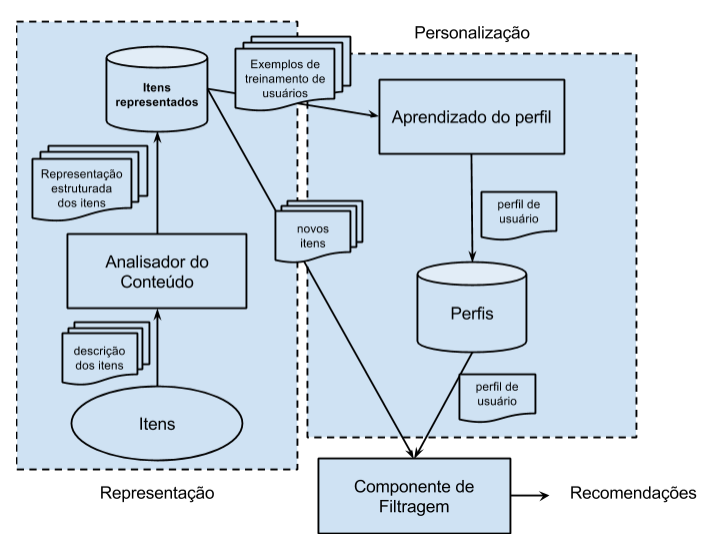
\includegraphics[width=100mm]{img/approach.png}
\caption{Arquitetura de um CBRS}
\label{fig:approach}
\end{figure}

Essa arquitetura apresentada foi adaptada de \citeonline{Lops2011}, para maior compreendimento e maior adequação com esse trabalho.
As subseções~\ref{subsec:analisadorcontexto},~\ref{subsec:perfil} e~\ref{subsec:filtragem} fazem uma revisão da literatura das técnicas de Aprendizado de Máquina aplicadas aos módulos de um SRsbC.

\subsection{Analisador de Contexto}
\label{subsec:analisadorcontexto}

O Analisador de Contexto tem como função representar o item de uma maneira estruturada, a Figura~\ref{fig:analisador} explica como é construída essa etapa. A entrada são os itens, que são pré-processados, para então aplicar técnicas de Aprendizado de Máquina (Redução de Dimensionalidade ou Tarefas de Aprendizado de Máquina).
Esta etapa compreende o foco deste trabalho.

\begin{figure}[h]
\centering
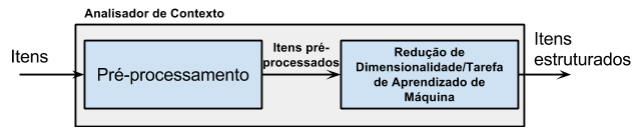
\includegraphics[scale=0.6]{img/analisador}
\caption{Analisador de Contexto.}
\label{fig:analisador}
\end{figure}

Na etapa de pré-processamento, é comum o uso da representação TF-IDF, sendo que existem estudos que propõem outros métodos de representação \cite{Capelle2012, Moerland2013}: SF-IDF (\textit{Semantics Frequency-Inverse Document Frequency}) e SF-IDF+, que obtiveram melhores resultados nos testes apresentados, além disso, \citeonline{Cleger2012} considerou o uso do TF-IDF, mas não resultou em melhores performances.
No entanto, em um SR no contexto de artigos científicos \cite{Beel2013}, foram realizados diversos testes considerando diversos parâmetros e configurações diferentes de representação, resultados mostraram que a configuração com TF-IDF performou melhor que outras.
Outras técnicas de Mineração de Dados também são utilizadas, como \textit{stopwords}, lematização e descarte de termos com frequência abaixo de um limiar.

Na etapa de Redução de Dimensionalidade/Tarefa de Aprendizado de Máquina faz-se o uso extensivo dos algoritmos: LSA (\textit{Latent Semantic Analysis}) \cite{Taraghi2013, Domingues2012, Spaeth2013}, LSI (\textit{Latent Semantic Indexing}) \cite{Saaya2013}, LDA (\textit{Latent Dirichlet Allocation}) \cite{Tantanasiriwong2012, Qu2012, Wang2012, Vaz2012}, que pode ser visto como uma extensão de Biclusterização \cite{Skillicorn2012}, e Variáveis Latentes \cite{Cleger2012}, que podem ser vistos por resolver uma tarefa de clusterização, que é agrupar termos em grupos que são chamados de tópicos \cite{Wang2012}.
O desafio é escolher o número de tópicos, por isso, grande parte dos trabalhos que fazem o uso dessas técnicas, realizam testes variando o número de tópicos.
Esses testes geralmente mostram que esses algoritmos ajudam na performance da recomendação \cite{Cleger2012, Tantanasiriwong2012, Saaya2013, Spaeth2013,Vaz2012}.

Na representação estruturada dos itens, alguns estudos propõem representações no contexto de notícias e artigos científicos \cite{Bielikova2012, Lops2013}: são diferenciadas as relevâncias de cada um dos atributos textuais (exemplo título, conteúdo, categoria e etc.), por meio de pesagem.
Estudos mostraram que com os pesos apropriados é possível melhorar a qualidade da recomendação.
Atributos que não são textuais também são usados no contexto de notícias, como no SR de notícias para celular em \cite{Yeung2012}, que o tempo da notícia modifica o vetor que representa o item, fazendo a multiplicação por um fator $\alpha$. o SR de livros \cite{Vaz2012} que tem como objetivo representar o estilo de escrita de cada autor, faz o uso de atributos como: o tamanho do documento, n-gramas e \textit{vocabulary richness}.

\subsection{Aprendizado do Perfil}
\label{subsec:perfil}

Nesta etapa é onde o perfil do usuário é representado e aprendido pelo SR. Na maioria das vezes o perfil é representado por um vetor de documentos de tamanho $k$, que o usuário visitou ou apresentou um feedback positivo $d_{prefs} = \{d_{pref_1}, d_{pref_2}, \dots, d_{pref_k}\}$.
Há outras formas de representação, como em \citeonline{Yeung2012}, que além da anterior, incorpora informações demográficas, tratando o problema de \textit{user cold-start} em SRsbC.
\citeonline{Vaz2012} propõem uma representação para o perfil do usuário usando um método da área de Recuperação de Informação: algoritmo de \textit{Rocchio}, onde cada documento $d_{pref_i}$ é classificado pelo usuário em positivo ou negativo (como exemplo, gostou ou não gostou), assim o algoritmo faz uma mistura dos objetos positivos e negativos, com um peso diferente para cada tipo de objeto, obtendo um vetor.
Então, esse vetor é comparado com vetores de itens (usando similaridade dos cossenos), para obter itens semelhantes.
Variando os parâmetros, os autores chegaram na conclusão que, incorporando objetos negativos na representação do perfil para treinamento do algoritmo, piora a qualidade das recomendações.

O aprendizado do perfil do usuário é como um problema de classificação, onde o vetor de objetos é dado por $X = \{d_{pref_i}, y^{+-}_i\}$, sendo que $y^{+-}_i$ representa o rótulo, ou seja, se $d_{pref_i}$ é um item que o usuário gostou($+$) ou não($-$).
Então, é treinado um classificador que irá classificar itens que o usuário ainda não consumiu, para saber se é um item que o usuário irá consumir/gostar.
Diversos algoritmos são usados para resolver esse tipo de problema: Redes Bayesianas \cite{Yeung2012, Cleger2012}, Naïve Bayes \cite{Lee2012, Semeraro2012}, SVM (\textit{Support Vector Machine}) \cite{Tantanasiriwong2012, Lee2012}.

Existem trabalhos que tratam o aprendizado do perfil com técnicas de Aprendizado Semi-Supervisionado, \citeonline{Lee2012} faz uso de comitê de máquinas para construir um modelo de Aprendizado de Máquina que classifica apenas classes positivas, visando classificar se o usuário de um e-commerce irá gostar ou não de um produto. Primeiramente, classifica objetos sem rótulo, para depois entrarem no modelo final que agrega todos os objetos (SVM ou Naïve Bayes).
Foi verificado que o SR proposto trata o problema de poucos dados para a identificação do perfil do usuário, pois não necessita apenas de dados rotulados.

É possível tratar o problema de aprendizado do perfil como um problema de clusterização \cite{Davoodi2012, Bielikova2012}.
\citeonline{Davoodi2012} apresentam um SR de especialistas, que representa o perfil dos usuários com semântica e constrói uma \textit{Rede Social}, para então, usar o algoritmo de clusterização (\textit{k-means}) para encontrar perfis de usuário.
Além desse, \cite{Bielikova2012} apresenta um SR de notícias que faz o uso de clusterização hierárquica, tendo como medidade de similaridade a similaridade dos cossenos e índice de jaccard.
Com uma abordagem \textit{bottom-up} de clusterização e uma estrutura de árvore binária, é realizado a clusterização das notícias: as folhas representam as notícias, e os nós pais, clusters que representam temas das notícias.
O usuário desse sistema é representado por caminhos nesta árvore construída, podendo ser recomendados diversas notícias dentro de diversos tópicos, que podem surpreender o usuário, amenizando o problema de serendipidade em SRsbC.

\subsection{Componente de Filtragem}
\label{subsec:filtragem}

Essa é a etapa mais simples, por ser na maioria das vezes, apenas uma filtragem das recomendações já calculadas na etapa de Aprendizagem do Perfil, essa estratégia é apresentada em \citeonline{Cleger2012, Qu2012, Wang2012, Davoodi2012, Mannens2011, Semeraro2012}. Outra estratégia simples é a determinação de um limiar \cite{Capelle2012, Lops2013}, ou seja, os valores da lista de recomendação gerada são filtradas pelo limiar estabelecido. Nos estudos apresentados, foram encontrados muitos SRs Híbridos, que faziam uma outra abordagem para a filtragem, usando uma combinação dos métodos de Filtro Colaborativo e baseados em conteúdo \cite{Lops2013, Qu2012, Domingues2012, Spaeth2013, Vaz2012}.

O trabalho desenvolvido por \citeonline{Bielikova2012} foi o único que apresentou uma estratégia diferente para o Componente de Filtragem, com a árvore binária montada, todas as notícias dos menores para os maiores grupos, que não foram lidas pelo usuário, foram separadas para a recomendação. Então, é construída uma matriz com as recomendações, sendo as linhas ordenadas pelos grupos menores para os grupos maiores, e as colunas ordenadas pelas notícias mais recentes. Assim, cada coluna é transformada em um vetor, concatenando-os e formando uma lista que é apresentada para o usuário.

\chapter{Proposta}

% essa parte você coloca no capítulo 4. Na proposta. Em algum lugar você vai dizer o que já foi feito então você pode dizer que acessou esse material na análise exploratória. Aqui é para falar qual é a metodologia, e não relatar o que já foi feito.

%Pa

%Isso tudo tem que vir no capitulo da propsota, como eu disse, aqui é não é um momento de relatar atividades realizadas.
%

%idem
%

%Para gerar conhecimento do corpus iG, serão aplicados algoritmos de Biclusterização que estão sendo implementados\footnote{https://github.com/lucasbrunialti/biclustering-experiments} nos textos das notícias processados e representados por diversas estratégias (TF-IDF, TF-IDF normalizado e n-gramas). Assim, será possível avaliar o resultado dos algoritmos utilizando a base de dados de cliques iG.

% A falta de serendipidade nas recomendações é um problema para SRs baseados em conteúdo.
% Biclusterização é uma técnica capaz de expandir as possibilidades de formação de clusters, levando em consideração a análise de subconjuntos de atributos para análise de similaridade entre dados a serem considerados como pertencentes a um cluster, ou bicluster.
% A possibilidade de considerar a análise de subconjuntos de atributos pode levar à descoberta de objetos similares, que não são necessariamente similares, quando todo o conjunto de atributos é considerado.
% Sendo assim, a hipótese formulada nesse projeto é que considerar similaridades parciais entre itens a serem recomendados pode melhorar a serendipidade das recomendações e, uma forma de implementar essa estratégia em SRs, seria por meio da aplicação de algoritmos de Biclusterização sobre o conjunto de itens a serem recomendados.

% \section{Objetivos}

% O objetivo geral desse trabalho é amenizar a dificuldade de oferecer recomendações com serendipidade em SRs que se baseiam no conteúdo textual.
% Esse objetivo deverá ser atingido por meio da aplicação de técnicas de clusterização de texto, em particular pela aplicação de algoritmos de Biclusterização.

% %Lucas, leia esse parágrafo abaixo com cuidado e reflita se é isso mesmo.
% A clusterização, nesse contexto, deve atuar como estratégia de organização do conteúdo textual, agrupando itens em biclusters.
% Sendo que a partir da observação dos interesses do usuário e dos biclusters à que estes itens pertencem, é possível organizar a lista recomendação com itens desses biclusters que esse usuário ainda não interagiu.

% Assim, com o intuito de melhor definir o contexto de estudo neste trabalho, foram estabelecidos os seguintes objetivos específicos:

% \begin{itemize}
%  \item Levantamento do referencial teórico de SRs.
%  \begin{itemize}
%   \item Levantamento do estado da arte sobre o uso de aprendizado de máquina na implementação de SRs baseados em conteúdo textual.
%  \end{itemize}
%  \item Levantamento do referencial teórico sobre Biclusterização e Mineração de Texto.
%  \item Construção de um corpus de itens textuais e um conjunto de dados de recomendação.
%  \item Implementação e teste dos algoritmos de Biclusterização sobre o corpus construído.
%  \item Modelagem do problema de recomendação baseado em conteúdo considerando a existência de biclusters de itens.
%  \item Análise da viabilidade da modelagem proposta frente ao conjunto de dados de recomendação e frente a análise qualitativa do alcance da serendipidade.
%  % \item estudo das técnicas de essemble aplicadas a texto
% \end{itemize}

% A fim de permitir os testes e validações sobre a modelagem a ser proposta para verificação da hipótese formulada neste projeto, faz-se necessário a definição de um contexto para realização de uma prova de conceito.
% Assim, foi escolhido usar o conteúdo referente à notícias publicadas no portal iG\footnote{http://ig.com.br/}.
% Trata-se de um portal de notícias brasileiro muito conhecido, com um volume de notícias bastante grande e com notícias categorizadas em canais, que representam os assuntos dessas notícias.
% Essas características conferem liberdade para a configuração de experimentos de diferentes naturezas, como experimentos considerando determinadas categorias de notícias, tipos de notícias ou datas de publicação das notícias.

% A partir do conteúdo de notícias do portal iG deve ser construído um corpus de dados textuais, categorizados de acordo com as categorias já usadas no referido portal.
% Todo o conteúdo do corpus deve passar por rotinas de pré-processamento comuns na área de Mineração de Texto: \textit{tokenização}, filtragem de \textit{stopwords}, remoção de sufixos (\textit{stemming}), representação da relação ``termos $\times$ documentos'' usando estratégias de frequência termos (TF-IDF) e \textit{n-grams}.

% %Leia com muito cuidado e veja se faz sentido. MUITO CUIDADO.ALTERE O QUE FOR NECESSÄRIOS TAMBÉM COM MUITO CUIDADO.
% Também, o portal iG possui informações históricas e anônimas referentes ao registro de navegação de usuários.
% Esse registro permite a construção de um conjunto de dados de preferências, que pode ser usado para realização de \textit{testes offline} entre recomendações oferecidas pela abordagem proposta e a navegação real realizada por um conjunto de usuários, utilizando métricas como precisão, revocação \cite{Jannach2011} e comparação com recomendações geradas por filtro colaborativo.

A proposta desse projeto de mestrado envolve a aplicação de algoritmos de Biclusterização para o problema de recomendação baseado em conteúdo textual, com a hipótese de que as recomendação geradas, possam amenizar o problema da serendipidade, visto que técnicas de Biclusterização são capazes de encontrar clusters através da análise de subconjuntos de atributos.

Formalmente, os algoritmos de Biclusterização irão atingir o módulo de representação dos itens em um SRsbC, mais especificamente, na função de similaridade entre itens $s: I \rightarrow I \times I$, que pode ser capaz de encontrar itens similares, que poderiam não ser similares caso $s$ fosse gerado por um algoritmo de clusterização, por exemplo.
Então, espera-se que o fator de mudança na função de similaridade entre itens $s$, acrescente um fator de serendipidade que influencie na aproximação da função $l_u$, que representa o perfil do usuário $u$, e portanto, na lista de recomendações $L_u$, direcionadas à $u$, dado que $l_u: \mathcal{H}_u, s \rightarrow L_u$, sendo $\mathcal{H}_u$ o subconjunto que representa o histórico de itens que $u$ acessou.

Então, para a validação dessa hipótese, se faz necessária a definição de um contexto para servir de prova de conceito.
Este contexto é referente à notícias presentes no portal iG\footnote{http://ig.com.br/}, um portal de notícias brasileiro muito conhecido, com um volume de notícias bastante grande e com alguma estrutura de classificação de notícias já existente.
Essas características conferem liberdade para a configuração de experimentos de diferentes naturezas, como experimentos considerando determinadas classes de notícias, tipos de notícias ou datas de publicação das notícias.

Como se tratam de notícias, é necessário fazer o uso de técnicas de Mineração de Texto para representar o conteúdo textual de notícias de maneira estruturada, possibilitando a construção de um corpus de notícias, que será usado para a validação da hipótese.
Para então, realizar a implementação de algoritmos de Biclusterização, que formarão biclusters para recomendar aos usuários, com base nos seus respectivos históricos $\mathcal{H}_u$.

Também, o portal iG possui informações históricas e anônimas referentes ao registro de navegação de usuários.
Esse registro permitirá a construção de um conjunto de dados de preferências, que poderá ser usado para realização de \textit{testes offline} para validar a prova de conceito, e portanto, a hipótese.

Os passos da proposta são sumarizados na Figura~\ref{fig:proposta}, onde se tem a fase de aquisição de notícias que comporá o corpus de notícias, para entrada na fase de pré-processamento, que utilizará de técnicas de Mineração de Texto para a estruturação do conteúdo textual, realizando diversas representações (TF-IDF, TF-IDF normalizado e \textit{n-grams}). Isso possibilitará a criação de biclusters através de algoritmos de Biclusterização, para então, dado o histórico de itens que o usuário navegou, analisar os biclusters que contém esses itens, e construir a lista de recomendação com base em outras notícias presentes nesses biclusters. Assim, será possível avaliar a qualidade dos biclusters gerados, em relação às notícias recomendadas e às informações históricas. Verificando também, como a estratégia se adequa à serendipidade, através da comparação das recomendações geradas pela estratégia por recomendações geradas através da técnica de filtro colaborativo.

\begin{figure}[h]
\centering
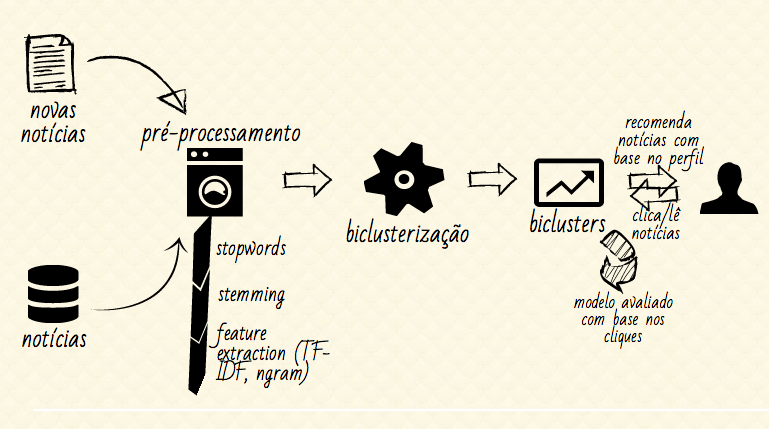
\includegraphics[width=120mm]{img/proposal.png}
\caption{Sumarização da proposta.}
\label{fig:proposta}
\end{figure}

Com o objetivo de especificar ainda mais as etapas da proposta e trazer informações sobre o desenvolvimento das mesmas, as seções Revisões Bibliográficas (Seção~\ref{sec:revisoesbibliograficas}), Construção das Bases de Dados (Seção~\ref{sec:basesig}), Estratégias para Validação e Extensões (Seção~\ref{sec:estrategiasvalidacao}) e Cronograma - Próximos Passos (Seção~\ref{misc:cronograma}) são apresentadas.

\section{Revisões Bibliográficas}
\label{sec:revisoesbibliograficas}

Se fez necessária, primeiramente, de uma análise exploratória para obter noções básicas da área de SRs, que foi realizada através da leitura de livros e artigos do tipo revisão bibliográfica, o que permitiu, em seguida, o aprofundamento na área de SRs, por meio da RS em Aprendizado de Máquina e SRsbC Textual.

A RS compreende estudos entre 2003 à 2014 que fazem referência ao estudo do estado da arte ou estado da prática sobre SRsbC textuais e apresentem alguma solução com o uso de técnicas de Aprendizado de Máquina.
Os estudos foram selecionados através da busca sistemática nas seguintes bases de dados: Scopus\footnote{http://www.scopus.com/}, ISI \textit{web} of Science (WoS)\footnote{http://apps.webofknowledge.com/}, IEEE Xplore\footnote{http://ieeexplore.ieee.org}, ACM Digital Library\footnote{http://dl.acm.org} e SpringerLink\footnote{http://link.springer.com/}. Para cada busca foi escrito um protocolo (veja um exemplo no Apêndice~\ref{app:protocolo}).
Para realizar a filtragem dos estudos encontrados foi utilizada uma abordagem \textit{Tollgate}: três pesquisadores aplicam os critérios de inclusão de maneira independente, e então, o consenso na decisão final é decidido pela maioria.
Sendo assim, a fim de extrair os dados dos estudos, é realizada a leitura dos estudos incluídos e seus dados sumarizados em uma tabela (veja um exemplo no Apêndice~\ref{app:protocolo-extracao}).

Com um total de $304$ estudos após a identificação nas bases de dados e remoção de duplicatas, foi feita a leitura e extração de dados de $18$ estudos, que compreendem os estudos publicados entre os anos de 2012 à 2014. A finalização da RS se dará após aplicação da filtragem e extração de dados para os demais anos.

Para aplicação dos algoritmos de Biclusterização, foi realizado um levantamento do referencial teórico, através da análise exploratória de livros, artigos do tipo revisão bibliográfica e artigos que se referem à criação dos algoritmos \cite{Franca2010,Cheng2000,Tanay2005,Madeira2004,Santamaria2007,Kluger2003,Prelic2006}.
Isso possibilitou a geração de conjuntos de dados sintéticos (Seção~\ref{sec:tiposbic}), e implementação do algoritmo de \citeonline{Cheng2000} nesses conjuntos, disponibilizado em \textit{https://github.com/lucasbruni\\alti/biclustering-experiments}.

Além disso, também foi necessária a realização de uma análise exploratória das áreas de Mineração de Texto, para que fosse possível a estruturação dos conteúdos textuais presentes nas notícias (Seção~\ref{sec:basesig}).

\section{Construção das Bases de Dados}
\label{sec:basesig}

\subsection{Corpus iG}
\label{subsec:corpusig}

A extração das notícias do portal iG foi realizada através da implementação de um \textit{web crawler} utilizando a linguagem python\footnote{https://www.python.org/}.
As notícias foram capturadas a partir de uma página de início, fornecida para o \textit{web crawler}, que era selecionada a fim de equalizar a distribuição de notícias por ano e por categoria (canal).

O corpus iG é composto por um conjunto de notícias do portal iG\footnote{http://www.ig.com.br/} $\mathcal{N} = \{ I_1, \dots, I_m,\\ \dots, I_M \}$, em que cada notícia $I_m$ é representada pela tupla $(\text{\textit{permalink}}, \text{\textit{título}}, \text{\textit{subtítulo}}, \text{\textit{corpo}},\\ c_i)$, em que $\text{\textit{permalink}}$ é o endereço eletrônico fixo da notícia, e, $c_i$ um elemento do conjunto de canais $\;\mathcal{C} = \{ \text{\textit{gente}}, \text{\textit{ultimosegundo}}, \text{\textit{delas}}, \text{\textit{economia}}, \text{\textit{esporte}}, \text{\textit{saude}}, \text{\textit{igay}}, \text{\textit{deles}},\\ \text{\textit{tecnologia}}, \text{\textit{igirl}}, \text{\textit{jovem}}, \text{\textit{arena}}, \text{\textit{luxo}} \}$, onde cada canal representa um assunto ou categoria de notícias.

O número total de notícias do corpus é $M = 4\;593$, com mais de $250$ caracteres no \textit{corpo}, no perído de 02 de Janeiro de 2012 à 11 de Outubro de 2014. As notícias estão bem distribuídas por ano: $1\;551$ notícias em 2012, $1\;933$ notícias em 2013 e $1\;109$ em 2014. Como cada notícia esta associada com um canal, foi coletada a distribuição de notícias por canal (Tabela 1).

\begin{table}[h]
\label{tab:distcanais}
\centering
\caption{Distribuição de notícias por canal ($ci$) do corpus iG.}
\begin{tabular}{c|c}
\hline
canal ($ci$)                    & número de notícias \\
\hline
$\text{\textit{gente}}$         & 196 \\
$\text{\textit{ultimosegundo}}$ & 555 \\
$\text{\textit{delas}}$         & 252 \\
$\text{\textit{economia}}$      & 907 \\
$\text{\textit{esporte}}$       & 342 \\
$\text{\textit{saude}}$         & 88  \\
$\text{\textit{igay}}$          & 210 \\
$\text{\textit{deles}}$         & 141 \\
$\text{\textit{tecnologia}}$    & 359 \\
$\text{\textit{igirl}}$         & 527 \\
$\text{\textit{jovem}}$         & 524 \\
$\text{\textit{arena}}$         & 421 \\
$\text{\textit{luxo}}$          & 71  \\
\hline
\end{tabular}
\end{table}

Analisando a distribuição de notícias por ano foi possível verificar que os links escolhidos como partida para o \textit{web crawler} realizar a extração de notícias foram efetivos para deixar a distribuição perto de uniforme, com média e desvio padrão de aproximadamente $1531 \pm 337$ notícias.
Contrariamente, a distribuição de notícias por canal não ficou perto do uniforme, com média e desvio padrão de aproximadamente $353 \pm 225$ notícias, uma hipótese é que isso se deve à idade e popularidade do canal, por exemplo, os canais $\text{\textit{luxo}}$ e $\text{\textit{deles}}$ são muito mais recentes e menos populares que o $\text{\textit{ultimosegundo}}$.

\subsection{Pré-processamento do corpus iG}

Com o corpus iG criado, o intuito da fase de pré-processamento é representar as notícicas de maneira estruturada, para isso foram utilizadas técnicas de Mineração de Texto (Seção~\ref{sec:mintexto}).
Foi criado um \textit{pipeline} para o pré-processamento das notícias que contou com as seguintes etapas:
% \begin{enumerate}[label*=\arabic*.]
%   \item Concatenação das características textuais (título, subtítulo e corpo da notícia) da notícia; normalização do texto, convertendo para minúsculo.
%   \item Filtragem de trechos do texto que correspondem com uma lista de expressões regulares definidas através da análise do corpus.
%   \item \textit{Tokenização}, usando espaços, pontuações e expressões regulares como delimitadores.
%   \item Definição de uma lista de \textit{stopwords}, a partir de uma lista já definida pela biblioteca nltk\footnote{http://www.nltk.org/} (\textit{Natural Language Processing Toolkit}) da linguagem python, foram adicionadas mais \textit{stopwords} à essa lista (por exemplo: \textit{leia mais}, \textit{veja aqui} e etc.), através de uma análise empírica das notícias do corpus.
%   \item \textit{Stemming}, para reduzir ambiguidade e a dimensionalidade das notícias, foi aplicado o algoritmo Removedor de Sufixos da Língua Portuguesa (RSLP) Stemmer \cite{Alvares2005}, que leva em consideração a teoria da língua portuguesa para criar 8 etapas, em que, cada etapa é composta por um conjunto de regras e então aplicada uma regra por vez. Este algoritmo é capaz de tratar e remover formas plurais, femininas/masculinas, adverbiais, aumentativas e diminutivas, substantivas, verbais e acentos.
%   \item Representação estruturada dos termos em:
%   \begin{enumerate}[label*=\arabic*.]
%     % \item TF
%     \item TF-IDF, realiza a contagem dos termos e aplica a fórmula de TF-IDF.
%     \item TF-IDF normalizado, realiza a contagem dos termos, aplica a fórmula de TF-IDF e faz a normalização para que todos os valores fiquem no intervalo de 0 à 1.
%     \item \textit{2-grams}, realiza a contagem dos termos concatenando 2 a 2.
%     % \item \textit{2-grams TF-IDF}, realiza a contagem dos termos concatenando 2 a 2.
%     \item \textit{3-grams}, realiza a contagem dos termos concatenando 3 a 3.
%   \end{enumerate}
% \end{enumerate}

\subsection{Base de cliques iG}
\label{subsec:basecliquesig}

A base de dados de cliques iG, doada para a realização deste trabalho, é composta por um conjunto usuários anônimos $U = \{ u_1, \dots, u_n, \dots, u_N \}$ que foram capturados através do controle de \textit{cookies} dos navegadores do portal, assim, cada usuário $u \in U$ interage com o conjunto de notícias $\mathcal{N}$ através de cliques, representados por $h_{u_n,I_m}^t$, um clique em uma notícia $I_m$ que foi dado por $u_n$ em um dado momento do tempo $t$.
Assim, se considerar cada clique $h_{u_n,I_m}^t$ como uma preferência do usuário $u_n$ por $n$, é possível construir a matriz de preferências $U \times I$ (Seção~\ref{sec:sr}), no contexto, $\mathcal{I} = \mathcal{N}$.

A base de cliques iG é composta de $487\;487\;395$ cliques, com notícias coletadas, aproximadamente, do período de abril de 2013 à novembro de 2014. Essa base de dados tem tamanho total, sem compressão, de $100GB$, o que dificulta a sua mineração. No entanto, pretende-se usar apenas as notícias que compõem o corpus iG.


\section{Estratégias para Validação e Extensões}
\label{sec:estrategiasvalidacao}

\subsection{Estratégias para Validação}

A primeira forma de avaliação do trabalho, consistirá na análise dos biclusters criados através de medidas de avaliação internas, onde usa-se os próprios biclusters, juntamente com métricas de qualidade e/ou estabilidade, para avaliar as soluções geradas.
A métrica estudada até o momento para avaliação interna é a métrica de consistência \cite{Santamaria2007}, que verifica se os biclusters encontrados correspondem com a definição de bicluster.

Também serão realizados \textit{testes offline}, utilizando a base de cliques iG, para verificar se o modelo proposto, é capaz de oferecer recomendações consistentes, comparando as recomendações geradas para um usuário $u$ com o histórico deste mesmo usuário, utilizando as métricas de precisão e revocação, variando o número de recomendações oferecidas.
Segundo \citeonline{Jannach2011}, essa estratégia é a que mais se adequa quando a recomendação é em forma de lista que é apresentado à um usuário.
Este método também pode ser interpretado como uma avaliação externa dos biclusters.

Ainda utilizando a base de cliques iG, será realizada outra avaliação com \textit{testes offline}, comparando as recomendações obtidas com recomendações geradas por um filtro colaborativo, que será, a princípio, implementado neste trabalho, fazendo uma comparação da recomendação gerada com a estratégia proposta e da recomendação gerada com o filtro colaborativo.
Serão utilizadas as mesmas métricas presentes na avaliação anterior.

\subsection{Possíveis Extensões}

Sobre a geração da lista de recomendações direcionadas à um usuário ($L_{u_n}$), uma forma mais simples, já descrita neste trabalho, é verificar os itens do histórico do usuário, buscando os biclusters aos quais esses itens pertencem, e dentro desses biclusters procurar por notícias para a construção da recomendação.
Uma possível abordagem para a geração de $L_{u_n}$ é observar o histórico de itens que o usuário $u_n$ interagiu, como um modelo escondido de Markov, em que deseja-se descobrir a probabilidade do próximo item que o usuário vai consumir: $P( h_{u_n,I_{m+1}} | h_{u_n,I_{1}},\dots,h_{u_n,I_{m}} )$, este modelo é chamado, especificamente, de \textit{Variable Length Markov Chains} \cite{Murphy2012}.
Ainda, é possível combinar os resultados dos biclusters com o modelo escondido de Markov, fazendo com que que esteo calcule a probabilidade do próximo bicluster em que o usuário irá navegar.

Outra possível extensão, diz respeito ao uso de \textit{Ensemble} de Clusterização \cite{Strehl2002}, como forma de substituir os algoritmos de Biclusterização, visto que estes podem considerar subconjuntos de atributos para a formação de clusters.
Assim, é possível fazer comparações com uma técnica semelhante à originalmente proposta: Biclusterização.

% ----------------------------------------------------------
% ELEMENTOS PÓS-TEXTUAIS
% ----------------------------------------------------------
\postextual
% ----------------------------------------------------------

% ----------------------------------------------------------
% Referências bibliográficas
% ----------------------------------------------------------
\bibliography{referencias}

% ----------------------------------------------------------
% Glossário
% ----------------------------------------------------------
%
% Consulte o manual da classe abntex2 para orientações sobre o glossário.
%
%\glossary

% ----------------------------------------------------------
% Apêndices
% ----------------------------------------------------------

% ---
% Inicia os apêndices
% ---
\begin{apendicesenv}

% Imprime uma página indicando o início dos apêndices
%\partapendices

%-------------------------------------------------------------------------
% Comentário adicional do PPgSI - Informações sobre ``apêndice''
%
% Para todos os captions/(títulos) (de seções, subseções, tabelas,
% ilustrações, etc):
%     - em maiúscula apenas a primeira letra da sentença (do título),
%       exceto nomes próprios, geográficos, institucionais ou Programas ou
%       Projetos ou siglas, os quais podem ter letras em maiúscula também.
%
% Todas  as tabelas, ilustrações (figuras, quadros, gráficos, etc. ),
% anexos, apêndices devem obrigatoriamente ser citados no texto.
%      - a citação deve vir sempre antes da primeira vez em que a tabela,
%        ilustração, etc., aparecer pela primeira vez.
%
%-------------------------------------------------------------------------
\chapter{Tabela Workshop}

\section*{Tabela Workshop}

\begin{longtable}{c|p{0.6\linewidth}}
\hline
Contextualização / motivação & Algoritmos de coclusterização tem o objetivo de encontrar grupos em uma matriz de dados. Tais grupos são chamados coclusters por se caracterizarem como um subconjunto de linhas e colunas, e podem apresentar sob diferentes tipos de organização. Especialmente, organizações nas quais diferentes coclusters possuem linhas e/ou colunas em comum (organização com sobreposição) podem ser úteis para diversas aplicações, como mineração de textos, filtro colaborativo, recuperação de informação, etc. \\
\hline
Problema de pesquisa & Encontrar coclusters organizados com sobreposição em uma matriz de dados esparsa contendo valores reais positivos que representam dados de um domínio de aplicação. \\
\hline
Objetivo geral & Propor estratégias algorítmicas baseadas em Fatoração de Matrizes (FM) que sejam capazes de encontrar coclusters organizados com sobreposição em uma matriz esparsa de valores reais positivos. \\
\hline
Trabalhos relacionados & Biclustering algorithms for Biological Data Analysis: A Survey - Survey em algoritmos de coclusterização/biclusterização. Discute diferentes organizações de coclusters e algoritmos para cada uma delas. Fast Nonnegative Matrix Tri-Factorization for Large-Scale Data Co-clustering - Apresenta algoritmos de FM para coclusterização em dados binários. Não trata coclusters organizados com sobreposição. Orthogonal nonnegative matrix tri-factorization for co-clustering: Multiplicative updates on Stiefel manifolds - Apresenta uma survey com algoritmos baseados em FM juntamente com um novo algoritmo que encontra coclusters ortogonais. Estes algoritmos não encontram coclusters organizados com sobreposição. \\
\hline
Justificativa e relevância & Problemas reais se manifestam em domínios que podem apresentar coclusters organizados com sobreposição sobre matrizes de dados esparsas. Um exemplo é a mineração de textos aplicada à agrupamento de notícias. A representação vetorial de textos (as notícias), conhecidamente, gera matrizes esparsas. Notícias podem ser agrupadas em diferentes grupos a depender de quais de suas características são analisadas. Tais fatores caracterizam o problema sob estudo neste projeto. \\
\hline
Proposta para Solução & Estão sendo desenvolvidos algoritmos utilizando técnicas de FM com o intuito de resolver o problema de encontrar coclusters organizados com sobreposição em domínio nos quais os dados se apresentam como uma matriz esparsa. \\
\hline
Dados & Estão sendo usados: dados sintéticos; dados de notícias da base de dados Reuters; dados de trabalhos acadêmicos da Rochester University; dados de notícias de um grande portal brasileiro; e um conjunto de dados (movie lens) para teste também na área de filtro colaborativo. \\
\hline
Forma de validação & Provas de correção e convergência dos algoritmos desenvolvidos; comparação e experimentação com os algoritmos presentes nos trabalhos correlatos. Avaliação via índices de validação de clustering e coclusterização. \\
\hline
Limitações & FM supõe que os dados e características são separáveis linearmente. Esta restrição não é garantida em problemas reais, mas não impede que soluções baseadas em FM gerem resultados úteis. \\
\hline
Resultados esperados & Contribuições científicas: desenvolvimento de algoritmos inéditos baseados em FM para coclusterização organizados com sobreposição em matrizes esparsas positivas.

\end{longtable}


\end{apendicesenv}
% ---


% ----------------------------------------------------------
% Anexos
% ----------------------------------------------------------

% ---
% Inicia os anexos
% ---
\begin{anexosenv}

% Imprime uma página indicando o início dos anexos
%\partanexos


%-------------------------------------------------------------------------
% Comentário adicional do PPgSI - Informações sobre ``anexo''
%
% Para todos os captions/(títulos) (de seções, subseções, tabelas,
% ilustrações, etc):
%     - em maiúscula apenas a primeira letra da sentença (do título),
%       exceto nomes próprios, geográficos, institucionais ou Programas ou
%       Projetos ou siglas, os quais podem ter letras em maiúscula também.
%
% Todas  as tabelas, ilustrações (figuras, quadros, gráficos, etc. ),
% anexos, apêndices devem obrigatoriamente ser citados no texto.
%      - a citação deve vir sempre antes da primeira vez em que a tabela,
%        ilustração, etc., aparecer pela primeira vez.
%
%-------------------------------------------------------------------------
% \chapter{Resumo das normas}
% \label{anexoA}

% Considerando a dificuldade para formatar um texto acadêmico sem conhecimento básico do conteúdo da norma NBR 14724 ``Informação e documentação – Trabalhos acadêmicos – Apresentação'', este anexo apresenta um resumo de alguns conceitos dessa norma, conforme publicada em julho de 2011. Sugere-se a leitura completa da norma para garantir que seu documento seja completamente aderente à mesma. Em alguns casos específicos, este anexo apresenta alguns ajustes da norma especificamente para o PPgSI.

% \section*{1 NBR 14724: estrutura e algumas descrições}

% A estrutura de uma tese, dissertação ou qualquer outro trabalho acadêmico, deve compreender elementos pré-textuais, elementos textuais e elementos pós-textuais, que aparecem no texto na seguinte ordem:

% \subsection*{1.1 Elementos pré-textuais}

% \begin{itemize}
%     \item Capa (obrigatório)
%     \item    Folha de rosto (obrigatório)
%     \item    Errata (opcional)
%     \item    Folha de aprovação (obrigatório)
%     \item    Dedicatória (opcional)
%     \item    Agradecimentos (opcional)
%     \item    Epígrafe (opcional)
%     \item    Resumo em língua vernácula (obrigatório)
%     \item    Resumo em língua estrangeira (obrigatório)
%     \item    Listas de ilustrações: lista de figuras, lista de algoritmos, lista de quadros, etc. (opcional)
%     \item    Lista de tabelas (opcional)
%     \item    Lista de abreviaturas e siglas (opcional)
%     \item    Lista de símbolos (opcional)
%     \item    Sumário (obrigatório)
% \end{itemize}

% \subsection*{1.2 Elementos textuais}

% \begin{itemize}
%     \item    Introdução
%     \item    Desenvolvimento
%     \item    Conclusão
% \end{itemize}

% \subsection*{1.3 Elementos pós-textuais}

% \begin{itemize}
%     \item    Referências (obrigatório)
%     \item    Apêndice (opcional)
%     \item    Anexo (opcional)
%     \item    Glossário (opcional)
% \end{itemize}

% \section*{2 Definições relacionadas a elementos pré-textuais}

% A seguir, são apresentadas algumas definições contidas na norma relacionadas a elementos pré-textuais.

% \subsection*{2.1 Capa}

% Elemento obrigatório, para proteção externa e sobre o qual se imprimem informações que ajudam na identificação e uso do trabalho, na seguinte ordem:
% \begin{enumerate}
%     \item Nome completo do autor: responsável intelectual do trabalho.
%     \item    Título principal do trabalho: deve ser claro e preciso, identificando o seu conteúdo e possibilitando a indexação e recuperação da informação.
%     \item    Subtítulo (se houver): deve ser evidenciada sua subordinação ao título principal, precedido de dois pontos (:).
%     \item    Número do volume (obrigatório apenas se houver mais de um volume, de forma que deve constar em cada capa a especificação do respectivo volume).
%     \item    Local (cidade) da instituição de apresentação.
%     \item    Ano do depósito (entrega).
% \end{enumerate}

\end{anexosenv}

%---------------------------------------------------------------------
% INDICE REMISSIVO
%---------------------------------------------------------------------
%%%%%MF\phantompart
%%%%%MF\printindex
%---------------------------------------------------------------------

\end{document}
